%\epigraphfontsize{\small\itshape}
%\setlength\epigraphwidth{8cm}
%\setlength\epigraphrule{0pt}
%\epigraphfontsize{\small\itshape}

%\epigraph{There are two possible outcomes: If the result confirms the hypothesis, then you've made a measurement. If the result is contrary to the hypothesis, then you've made a discovery.}{---\textup{ Enrico Fermi}}
%\epigraph{Everyone knows how useful it is to be useful. No one seems to know how useful it is to be useless.}{---\textup{  Chuang Tzu, The Useless Tree}}
\section{An Overview of the Reconstruction Algorithms in SNO+}

A particle interaction that happens in the SNO+ detector can produce Cherenkov or scintillation photons or both. These photons propagate through the detector, and may trigger PMTs when they reach the PSUP. As described in the last chapter, if sufficiently many PMTs are triggered within a defined time window, an `event' is determined by the trigger system to have occurred, and the time and charge information measured by the hit PMTs are recorded.

By utilizing the recorded time and charge information, reconstruction algorithms attempt to calculate the physical quantities underlying (i.e. causing) the, including the event position and time (the ``vertex''), the direction of motion of the charged particle that prompted the primary light emission, and its energy. Several reconstruction algorithms (called ``fitters'') have been implemented in the SNO+ RAT software, or are still being developed. These fitters are based on differing methods, and can be coordinated and optimized for different detector situations or physics phases.

According to the physics quantities they determine, the SNO+ fitters can be generally classified as:
\begin{itemize}
	\item Vertex fitter. A vertex fitter reconstructs the event position and time by utilizing the positions and timing information of the hit PMTs. Currently, vertex fitters have been used to process the data and simulations for the water and partial-fill phases. They are also ready for the scintillator and tellurium-loading phases.
	
    On the other hand, some types of events, such as radioactive background events that emit $\gamma$-particles, can create multiple correlated vertices. A multi-site or multi-vertex fitter will be helpful in tagging and removing such types of events during the $0\nu\beta\beta$ search. This kind of fitter is being developed.

	\item Direction fitter. A direction fitter reconstructs the event direction by using the information encoded in the spatial distribution of the detected Cherenkov photons, which cause ring-like patterns of hit PMT positions. The direction fitter has been used in the water phase analysis. However during the scintillator and tellurium-loading phases the Cherenkov patterns will be submerged in scintillation photons, so that direction reconstruction requires a different approach, which is being developed currently. 
	
	\item Energy fitter. An energy fitter translates the number of photons created from an event to kinetic energy. Similar to the vertex fitters, the energy fitters currently have been used in the water and partial-fill phases, and they are ready for the scintillator and tellurium-loading phases.

	\item Muon track fitter. This fitter is used to reconstruct the tracks of cosmic muons. Each muon track is treated as a straight line, and by dividing the SNO+ detector into several XY-slices along Z, the fitter reconstructs the path's intersection point on each slice by utilizing the position and timing information of the set of hit PMTs\cite{muonTrackRecon}. The muon track fitter is currently being developed for the scintillator and tellurium-loading phases, and will help to tag and reduce the cosmogenic backgrounds, especially the $^{11}$C backgrounds induced by muon spallation on the liquid scintillators \cite{sorensen2016temperature}.
\end{itemize}

A fitter's performance is first tested on Monte Carlo simulations of specific physics processes, then on both simulations and data from the calibration runs. Once the algorithm has been proven to give good results and is approved by the SNO+ collaboration, it is implemented into the SNO+ RAT software to process the SNO+ simulations and data files.

For a specific SNO+ physics phase, the fitters for reconstructing different physics quantities of an event are integrated. Currently, there are three integrated fitters: the \texttt{Water Fitter} for the water phase, the \texttt{Partial Fitter} for the partial-fill phase, and the \texttt{Scint Fitter} for the scintillator phase and the tellurium loading phase. The fitter parameters, such as the optical parameters, fitter optimization parameters, are coordinated and optimized based on simulations and calibration data from that specific physics phase. In addition, PMT selectors and classifiers are also included in the integrated fitters. The PMT selectors are used to remove the outliers of the hit PMTs for a specific fitter, such as PMTs whose hit(s) probably were triggered by noise. These selectors can help to make the fitter more accurate or to boost fitter speed. The classifiers mainly use the reconstructed results to calculate specific quantities which describe the probability of determining an event as an expected signal or background.

In this chapter, a Multi-path (MP) reconstruction framework and its principles are discussed.It was developed by the University of Alberta group as an additional fitter to provide event vertex and direction reconstructions. In this framework, the fitters can be adapted for all the SNO+ physics phases by switching light path calculations, input parameters such as the optical parameters, and the detector state. That is the reason why it is called ``multiple paths''.  It was applied in the water phase to provide an alternative diagnosis of event position and direction; it also works as the vertex reconstruction algorithm for the \texttt{Partial Fitter}. After re-coordination for the scintillator and tellurium loading phases, I also show the potential of the vertex fitter for application in these two future phases.
\section{Multi-path Vertex and Direction Reconstructions for the Water Phase}\label{sect:mpw}

In the SNO+ water phase, both the cavity and the AV were filled with ultra-pure water. In this case, the detector geometry is simple since everything inside the PSUP sphere can be simplified as water (if one neglects the effects of the plexiglass AV shell). Therefore to explain the reconstruction concepts, I will start with the \texttt{MP water fitter} (the \texttt{MPW fitter}).

The \texttt{MPW fitter} determines the vertex and direction of a triggered event in the SNO+ water phase. It first fits for the event vertex and then uses that result (reconstructed position) to fit for the event direction.

\subsection{Vertex Reconstruction}\label{sect:waterVertex}

The vertex is defined by four parameters, namely $x,y,z$ and $t$. The fitter first creates a randomly-generated position inside a sphere of radius $10$ m (i.e. larger than the PSUP radius $r_{\mathrm{PSUP}}=8.39~$m). Meanwhile, a random event time $t_0$ (relating to the global trigger time) is also generated from a uniform distribution in the range of $[100,300]$~ns. The Class Library for High Energy Physics (\texttt{CLHEP}) is used for creating pseudo-random numbers. The random position and the random time are combined to form a random event vertex as the trial event vertex $(\vec{X}_0,t_0)$. Details are given in the Appendix.~\ref{appendix:random_gen}.

For each triggered event, photons created around the event position propagate to the hit PMTs. In a simplified detector geometry model that neglects the effects of scattering, reflection, and refraction, these photons are considered as propagating along straight lines that connect the trial event vertex to the hit PMTs. Thus the fitter evaluates a timing parameter, called the time residual ($t_\mathrm{res}$), which is defined as:
\begin{equation}
\label{eq:tres_define}
t_\mathrm{res}=t_\mathrm{PMT} - t_{\mathrm{transit}} - t_{\mathrm{event}},
\end{equation}
where $t_\mathrm{PMT}$ is the PMT trigger time recorded by the detector, $t_{\mathrm{event}}$ is the time when an event occurs (event time), and $t_{\mathrm{transit}}$ is the total transit time (or time of flight, TOF) taken by a photon traveling from the event position ($\vec{X}_{\mathrm{event}}$) to the hit PMT ($\vec{X}_{\mathrm{PMT}}$) and crossing different materials in the detector.

To calculate $t_{\mathrm{transit}}$, the fitter uses Cherenkov photons in a prompt time window (called the ``prompt light''), chosen as $-10<t_{\mathrm{res}}<10$ ns for the \texttt{MPW fitter}, and the photons are assumed to propagate in straight lines (straight light paths). By assuming straight light paths, or rather, by neglecting that they are {\em not} perfectly straight, complicated aspects of photon propagation are neglected, including refraction and reflection when photons cross boundaries between different detector materials, absorption and scattering by the detector medium, and the lensing effects caused by the spherical structure of the acrylic vessel. In this case, the TOF can be simply calculated as 
\begin{equation*}
t_{\mathrm{transit}}=\frac{|\vec{X}_{\mathrm{event}}-\vec{X}_{\mathrm{PMT}}|}{v_{\mathrm{water}}} \, 
\end{equation*}
where $v_{\mathrm{water}}$ is an effective average photon group velocity obtained by tuning on Monte Carlo simulations. Sect.~\ref{sect:tuneGroupVelocity} will show the details of this tuning. Based on reconstruction experience from the SNO experiment, it is found that even without the detailed tuning of $v_{\mathrm{water}}$ the fitter still produces results that are rather consistent with the outcome that {\em does} use a more detailed calculation \cite{boulay2004direct,jones2011background}. Fig.~\ref{mpwdiagram_position} shows straight light paths from the event position to the hit PMT positions.
\begin{figure}[htbp]
	\centering
   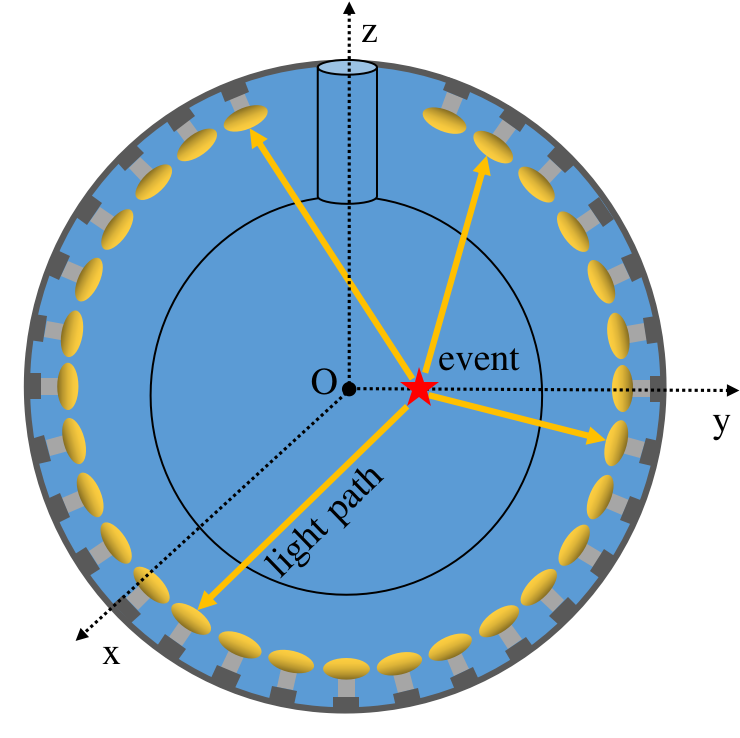
\includegraphics[width=6cm]{mpwDiagram_coord.png}
	\caption[Straight light path calculation in the water geometry.]{A diagram of straight light paths for event position reconstruction in the SNO+ water phase geometry.}
	\label{mpwdiagram_position}
\end{figure}

A one-dimensional (1D) probability density function (PDF) is used for fitting the timing model, as shown in Fig.~\ref{fig:MPW_timingPDF}. This PDF serves as a model of the timing responses of the triggered PMTs to the event being fitted. It was taken from the bench-top measurements of the individual PMT time profile from SNO \cite{jillings1996photomultiplier}, and was further tuned according to the measured \emph{in-situ} SNO+ detector response to the calibration sources \cite{anderson2021optical}.

\begin{figure}[!htb]
	\centering
	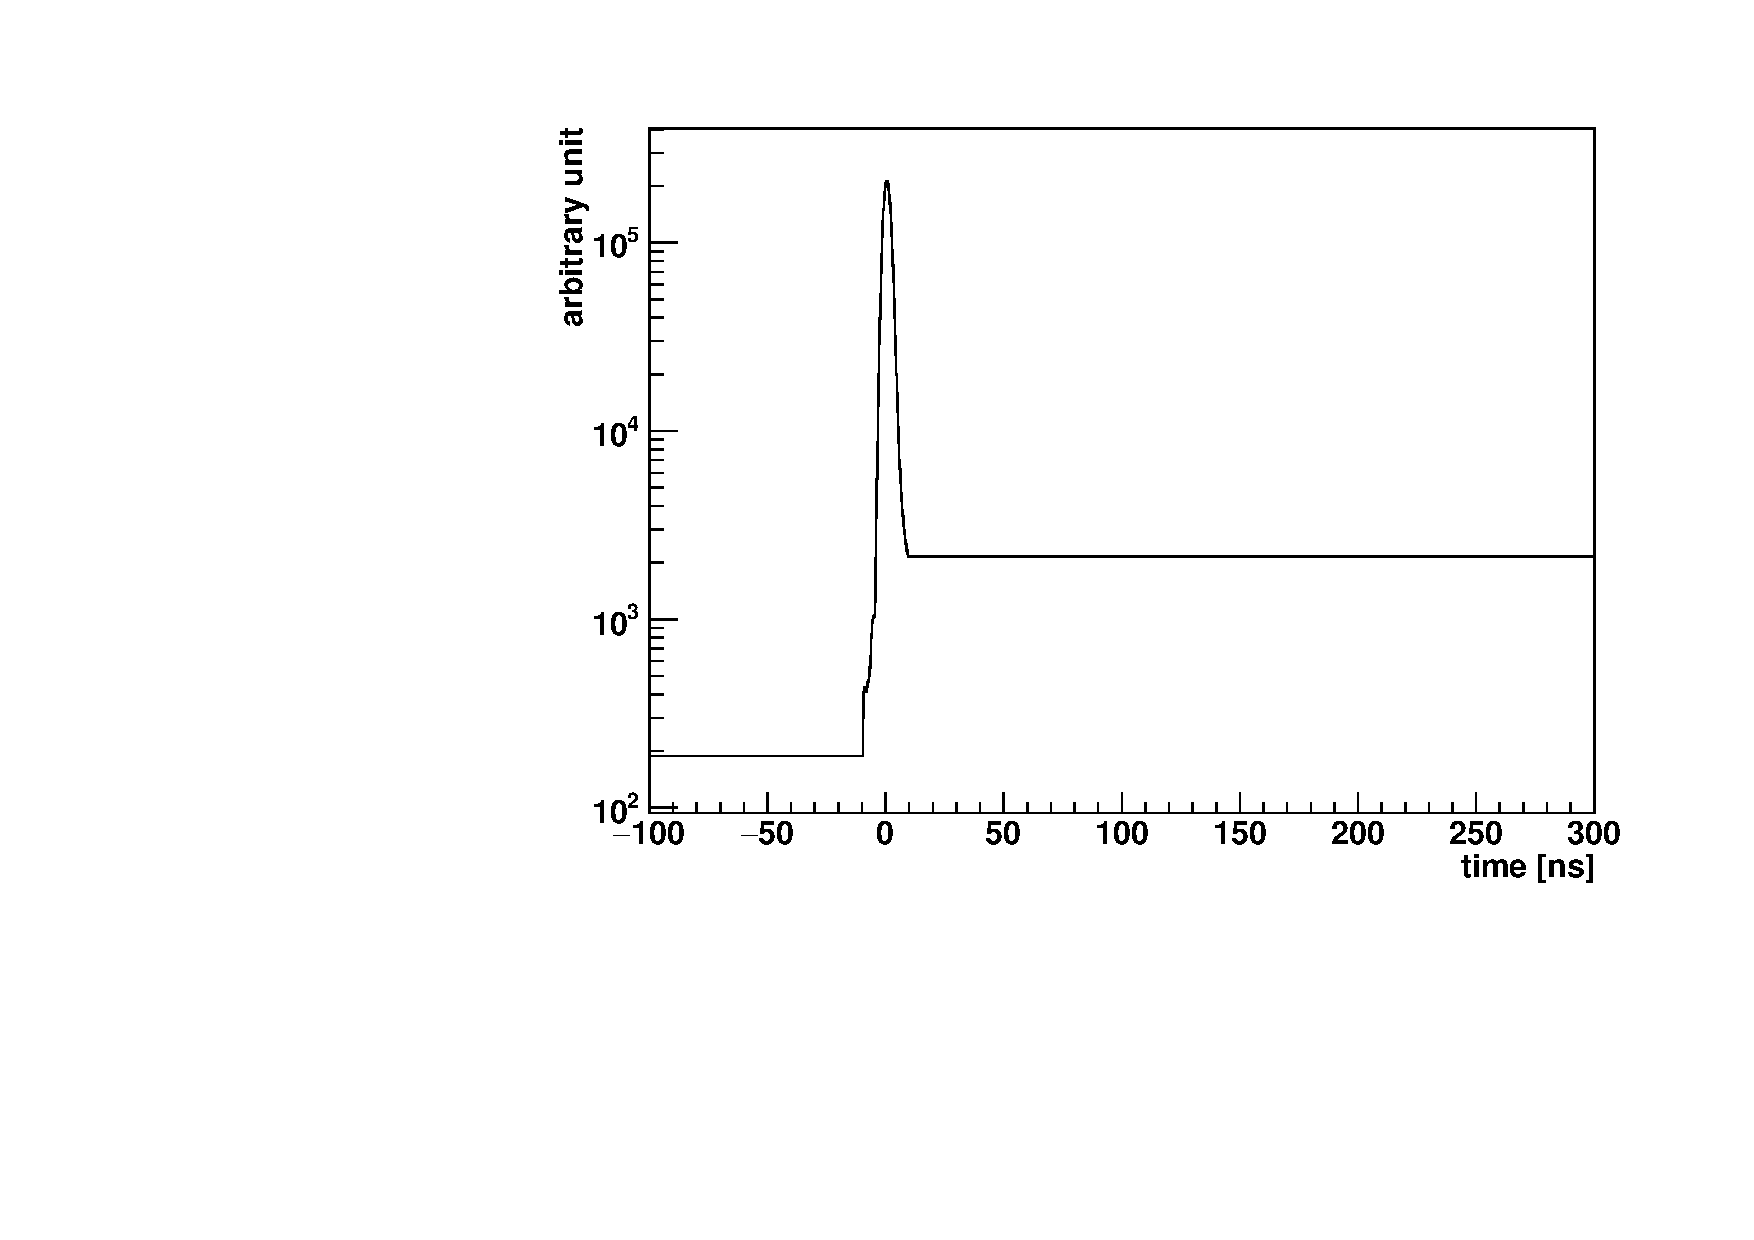
\includegraphics[width=10cm]{MPW_timingPDF.pdf}
	\caption{The PMT response time profile, used as the timing PDF for vertex reconstruction.}
	\label{fig:MPW_timingPDF}
\end{figure}

For a trial vertex $(\vec{X}_0,t_0)$, the fitter calculates a $t_{\mathrm{res}}$ value with respect to each hit PMT. Looping over all the hit PMTs, a likelihood function is built as:
\begin{equation}\label{eq:vertexLogL}
\ln\mathcal{L}(\vec{X}_0,t_0)=\sum_{i=1}^{{\mathrm{NHits}}}\ln P(t^i_{\mathrm{res}}),
\end{equation}
where $t^i_{\mathrm{res}}$ is the time residual calculated from the $i^{th}$ hit PMT; NHits is the total number of PMTs triggered by an event and $P(t^i_{\mathrm{res}})$ is the probability returned by reading the PDF when given a $t^i_{\mathrm{res}}$ for the $i^{th}$ hit PMT.

In summary the likelihood function starts with a random ($\vec{X}_0,t_0$) as a seed and calculates the likelihoods and their derivatives for various paths, assuming straight-line paths of the prompt Cherenkov light from the trial vertex $(\vec{X}_0,t_0)$ to each of the hit PMTs. The trial vertex is varied until the likelihood function reaches the global maximum, which corresponds to the best-fit vertex. This fitting scheme implements the Levenberg-Marquardt (MRQ) method, which is commonly used for fitting a nonlinear model with multiple parameters. In Sect.~\ref{appendix:MRQ} this method is described in detail, along with its application for the \texttt{MP fitter} (also see Refs.~\cite{gregory2005bayesian, press2007numerical} for details).

As will be shown in the sections to follow, one of the main tasks for the fitter is to calculate $t_{\mathrm{transit}}$ by evaluating light paths. As mentioned earlier, the water phase geometry is the simplest case compared to the other situations when the AV is filled with the wavelength shifter or scintillator. Such materials, with properties quite distinct from the cavity water, make the light path calculations more complicated.

\subsection{Direction Reconstruction}\label{sect:waterDirection}

A unit vector $\vec{u}$ with prescribed orientation can be defined by two parameters, the zenith angle $\theta$ and the azimuth angle $\phi$. In the Cartesian coordinate system, we have: 
\begin{equation}
\vec{u}=(\cos\phi\sin\theta,\sin\phi\sin\theta,\cos\theta) \;, 
\end{equation}
which is easily seen to have unit magnitude.

\begin{figure}[htbp]
	\centering
	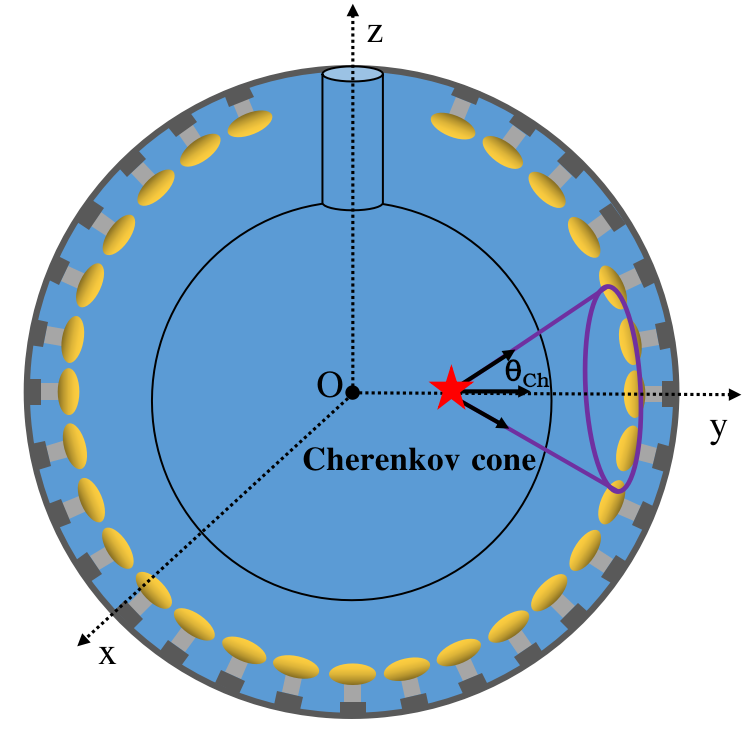
\includegraphics[width=6cm]{mpwDiagram2_coord.png}
	\caption[Cherenkov cone and straight line light paths (SNO+ water phase).]{Cherenkov cone and straight line light paths, in the SNO+ water phase geometry.}
	\label{mpwdiagram_direction}
\end{figure}
To fit for the direction with its two parameters ($\theta$, $\phi$), as for the vertex reconstruction a random trial direction $\vec{u}_0(\phi_0,\theta_0)$ is first generated using \texttt{CLHEP} (see Sect.~\ref{appendix:random_gen}). The direction fitter then evaluates an angular parameter, $\cos\theta_{\mathrm{Ch}}$, which is the angle between $\vec{u}_{0}$ and $\vec{X}_{\mathrm{diff}}\equiv \vec{X}_{\mathrm{event}}-\vec{X}_{\mathrm{PMT}}$. Therefore, the direction fitter requires an event position as input, and necessarily runs after the vertex fitter\footnote{It has been discussed that, instead of fitting in two steps, the vertex and direction can be fitted simultaneously by utilizing the MRQ algorithm for fitting six parameters ($x,y,z,t,\theta,\phi$). However results were worse by using this method.}.

A 1D PDF, serving as a model of the angular distribution of the triggered PMTs and shown in Fig.~\ref{fig:MPW_angularPDF}, is used for fitting the angular model. It was obtained from 10000 MC simulations of 5-MeV $e^-$ events generated at the detector center ($\vec{X}_{MC}=(0,0,0)$), and traveling along the positive side of the $x$-axis, i.e., the orientation of the momentum vector is $\vec{u}_{\mathrm{MC}}=(1,0,0)$\footnote{Here 5 MeV is a typical energy for the SNO+ water phase analysis. No obvious changes in fitter performances by using PDFs generated with alternative values for electron energy.}.

\begin{figure}[!htb]
	\centering
	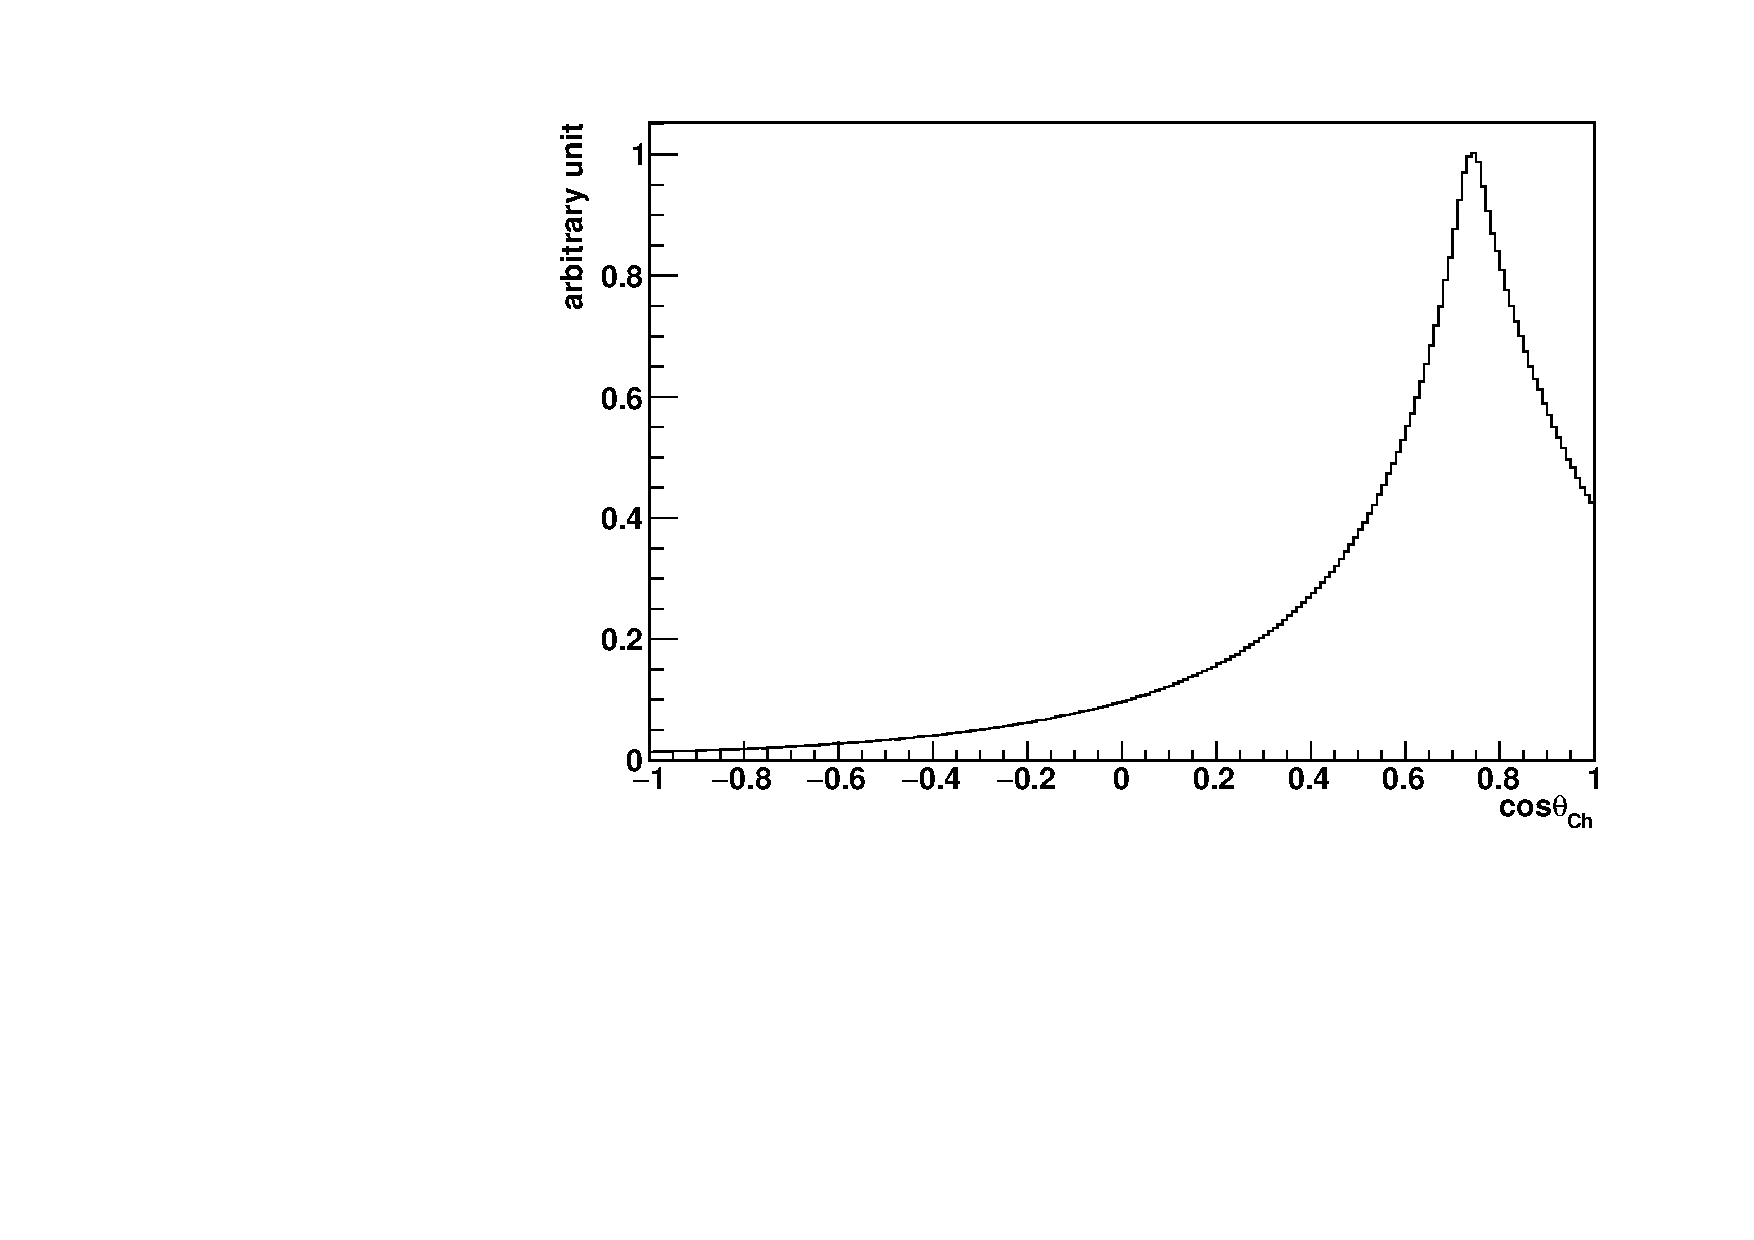
\includegraphics[width=10cm]{MPW_angularPDF.pdf}
	\caption{PMT angular distribution as the angular response PDF for direction reconstruction.}
	\label{fig:MPW_angularPDF}
\end{figure}

For the $i^{th}$ hit PMT, $\cos\theta^i_{\mathrm{Ch}}=\vec{u}_0\cdot\frac{\vec{X}^i_{{\mathrm{diff}}}}{|\vec{X}^i_{{\mathrm{diff}}}|}$, then the likelihood function is built as:
\begin{equation}
\ln \mathcal{L}(\vec{u}_0)=\sum_{i=1}^{{\mathrm{Nhits}}}L_i(\cos\theta_{\mathrm{Ch}}^i),
\end{equation}

Finally, the fitter fits for the angular PDF by using the MRQ method to obtain the best-fit direction. There are several optimizations for improving the fitter performance. First, the group velocity used in the $t_{\mathrm{transit}}$ calculation is tuned, as shown in Sect.~\ref{sect:tuneGroupVelocity}. In Sect.~\ref{sect:fitterPull}, a drive correction for compensating the pulls in the reconstructed position is discussed. In Sect.~\ref{sect:PMTselector}, PMT selectors for sending proper PMT information to the fitter are discussed. 

\subsection{Effective Group Velocity}\label{sect:tuneGroupVelocity}

When photons travel through the detector, their group velocities ($v_\mathrm{gr}$) change in accordance with the different refractive indices of different detector materials. The group velocities also depend on the wavelengths of the photons: $v_\mathrm{gr}=c/n(\lambda)$. Fig.~\ref{nVsWavelength} shows the measured refractive index ($n$) of water as a function of wavelength, obtained from the measurements of the laserball scans in the SNO+ water phase\cite{laserball_groupVelocity}. %Furthermore, $v_\mathrm{gr}$ can change when photons are scattered, absorbed, refracted and reflected in the detector.

\begin{figure}[!htb]
	\centering
	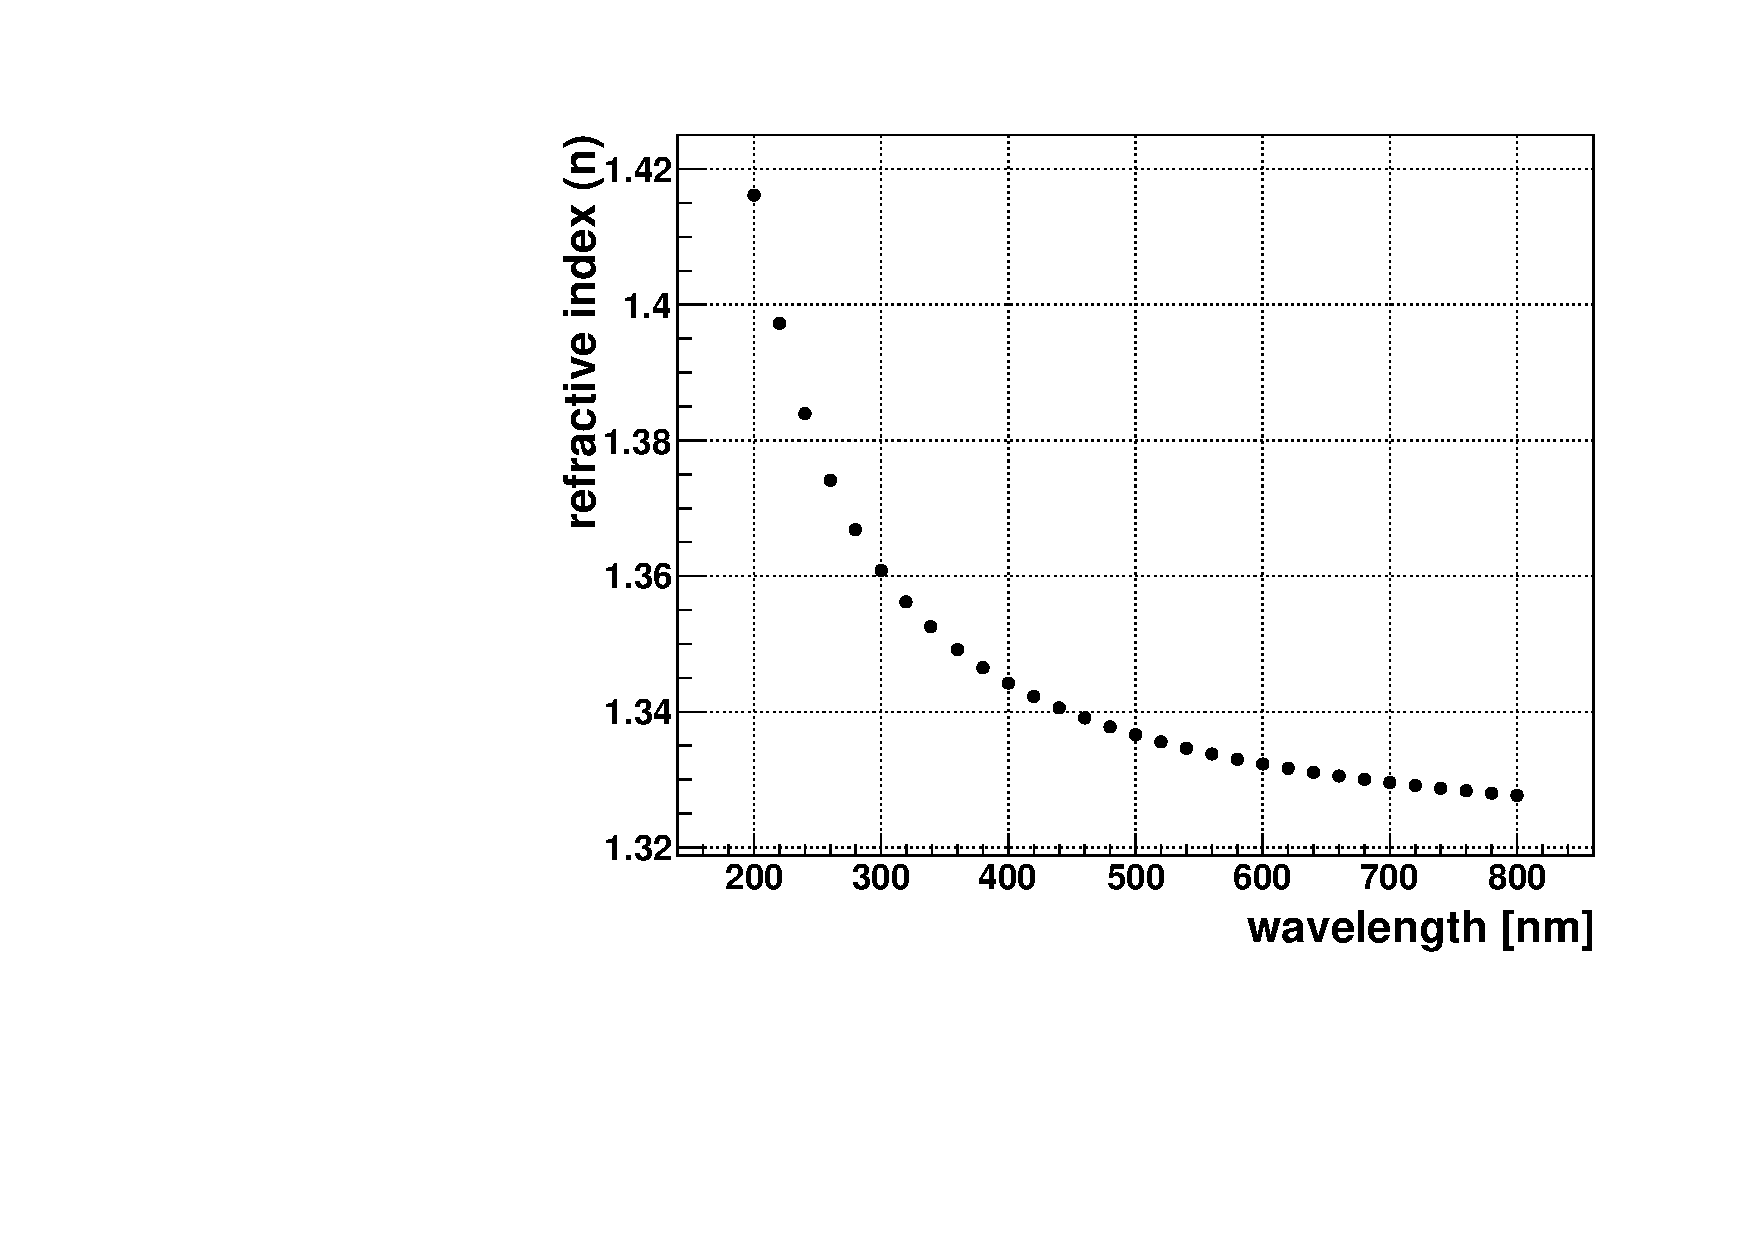
\includegraphics[width=6cm]{refractiveIndexVsWavelength.pdf}
	\caption[Refractive index of water vs wavelength.]{Refractive index of water vs wavelength, reproduced from \texttt{RAT}. These values are based on the measurements from laserball calibration scans in the SNO+ water phase\cite{laserball_groupVelocity}.}
	\label{nVsWavelength}
\end{figure}

To simplify reconstruction, a tuned value (of $v_\mathrm{gr}$) is used in the straight line light path calculation. As mentioned in Sect.~\ref{sect:mpw}, the water vertex fitter calculates $t_\mathrm{transit}$ by evaluating the distances from the trial vertex to the hit PMTs: $t_\mathrm{transit}=|\vec{X}_\mathrm{event}-\vec{X}_\mathrm{PMT}|/v_\mathrm{gr,eff}$, where the $v_\mathrm{water}$ is replaced by the effective group velocity $v_\mathrm{gr,eff}$. The value of $v_\mathrm{gr,eff}$ set in the fitter can introduce bias in the reconstructed position, mainly due to a ``complementary'' effect of the fitter. Setting a large value of $v_\mathrm{gr,eff}$ (a fast effective group velocity) will decrease $t_\mathrm{transit}$, while according to Eqn.~\ref{eq:tres_define}, $t_\mathrm{res}$ will increase. During the reconstruction, when the fitter compares the large $t_\mathrm{res}$ with the timing PDF, it will attempt to place the trial vertex further away from the hit PMTs to increase $t_\mathrm{transit}$ and then decrease $t_\mathrm{res}$, as illustrated in Fig.~\ref{fig:effectiveVg}. On the other hand, if $v_\mathrm{gr,eff}$ is set too small (i.e. too slow), $t_\mathrm{transit}$ will increase while $t_\mathrm{res}$ will decrease, and the fitter will place the trial vertex closer to the hit PMTs to increase $t_\mathrm{res}$. These effects can be quantified as radial bias ($r_\mathrm{bias}$), which is the difference between the reconstructed and true (MC) positions ($\vec{X}_{fit}-\vec{X}_{MC}$), projected along the radial component of the true position (the unit vector $\hat{X}_{MC}$) \cite{coulter2013modelling}:
\begin{equation}
r_\mathrm{bias} \equiv (\vec{X}_{fit}-\vec{X}_{MC})\cdot \hat{X}_{MC}.
\end{equation}

\begin{figure}[!htb]
	\centering
	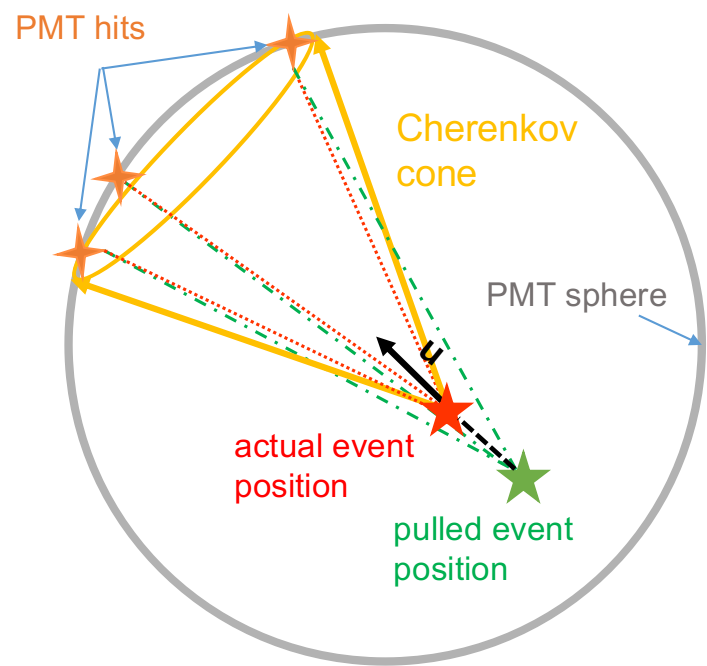
\includegraphics[width=6cm]{effectOfGroupVelocity.png}
	\caption[A cartoon shows effects of tuning the effective group velocity.]{A cartoon shows effects of tuning the effective group velocity. In this case, the effective group velocity is faster than expected, and the fitted position is dragged back along the direction to increase $t_\mathrm{transit}$.\label{fig:effectiveVg}}
\end{figure}
An overestimated $v_\mathrm{gr,eff}$ (too fast) results in a positive radial bias to the true event position while an underestimated one (too slow) brings a negative radial bias.

In practice, $v_\mathrm{gr,eff}$ is calculated by an effective refractive index $n_\mathrm{eff}$ (or `$RI$ value'): $v_\mathrm{gr,eff}=c/n_\mathrm{eff}$. To obtain a reasonable $v_\mathrm{gr,eff}$ for the water-phase vertex fitter, my initial approach was to obtain the value by a linear interpolation based on MC simulations. First, 500 simulations of 5-MeV electrons were generated uniformly inside the AV, with isotropic momentum directions. Then the \texttt{MPW fitter} reconstructed the same MC simulations by using seven different values of $v_\mathrm{gr}$, from 200 to 230 mm/ns (such that $n_\mathrm{eff}$ ranged from 1.50 to 1.30), with a step of 5 mm/ns. The distributions of radial bias from each reconstruction result were calculated and fitted with Gaussian functions. The mean values of these Gaussian fits were taken as the values of $r_\mathrm{bias}$, and they were plotted against $v_\mathrm{gr}$, as shown in Fig.~\ref{fig:plotVgr}. A linear fit was applied on these points, giving $v_\mathrm{gr,eff}=215.868\pm 5.585$ mm/ns ($n_\mathrm{eff}=1.3888$) at the point where $r_\mathrm{bias}=0$.

\begin{figure}[!htb]
	\centering
	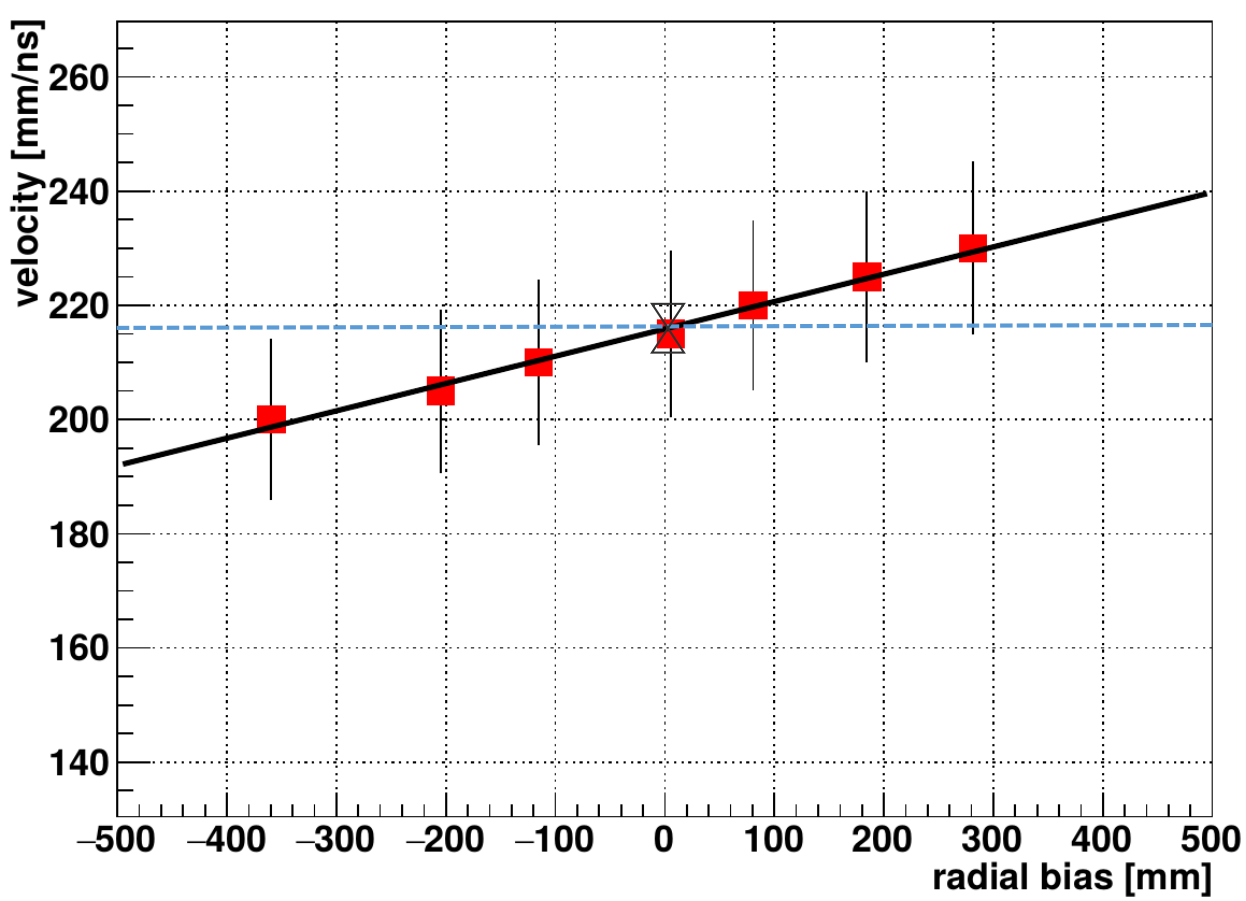
\includegraphics[width=6.5cm]{tune_groupVelocity_MPW.png}
	\caption[Group velocity vs. radial bias for the \texttt{MPW fitter}.]{Group velocity vs. radial bias for the \texttt{MPW fitter}.	\label{fig:plotVgr}}
\end{figure}

Later I turned to a more data-driven approach rather than only tuning from the simulations. This approach is to extract an average group velocity by analyzing the $^{16}$N calibration source data. As shown in Fig.~\ref{fig:n16_groupVeloctiy}, for the $^{16}$N central run-100934 and run-107055, the source was deployed almost at the PSUP center, and the optical photons propagated to reach PMTs on the PSUP. 

For each event, suppose the triggered PMTs were found within a solid angle
\begin{equation*}
\Omega=\frac{\pi(L/2)^2}{r^2_\mathrm{PSUP}}\; ,
\end{equation*}
where $L$ is the line segment and $r_\mathrm{PSUP}=8390$ mm is the radius of the PSUP, as shown in Fig.~\ref{fig:n16_groupVeloctiy}. Since the diameter of the PMT concentrator is 27 cm, the line segment is chosen as $L = 50$ cm ($\theta=\arcsin(\frac{1}{2}L/r_\mathrm{PSUP})\approx 0.17^\circ$) to let roughly 2 triggered PMTs be within the $\Omega$ (these PMTs are called `PMTin$\Omega$'). Then the arrival time $T_1$ was found by calculating $|\vec{X}_\mathrm{source}-\vec{X}_\mathrm{PMTin\Omega}|/v_\mathrm{water}$, where $v_\mathrm{water}=217.554$ mm/ns is an effective velocity obtained by the SNO+ collaboration for light in water \cite{coulter2013modelling}.

\begin{figure}[!htb]
	\centering
	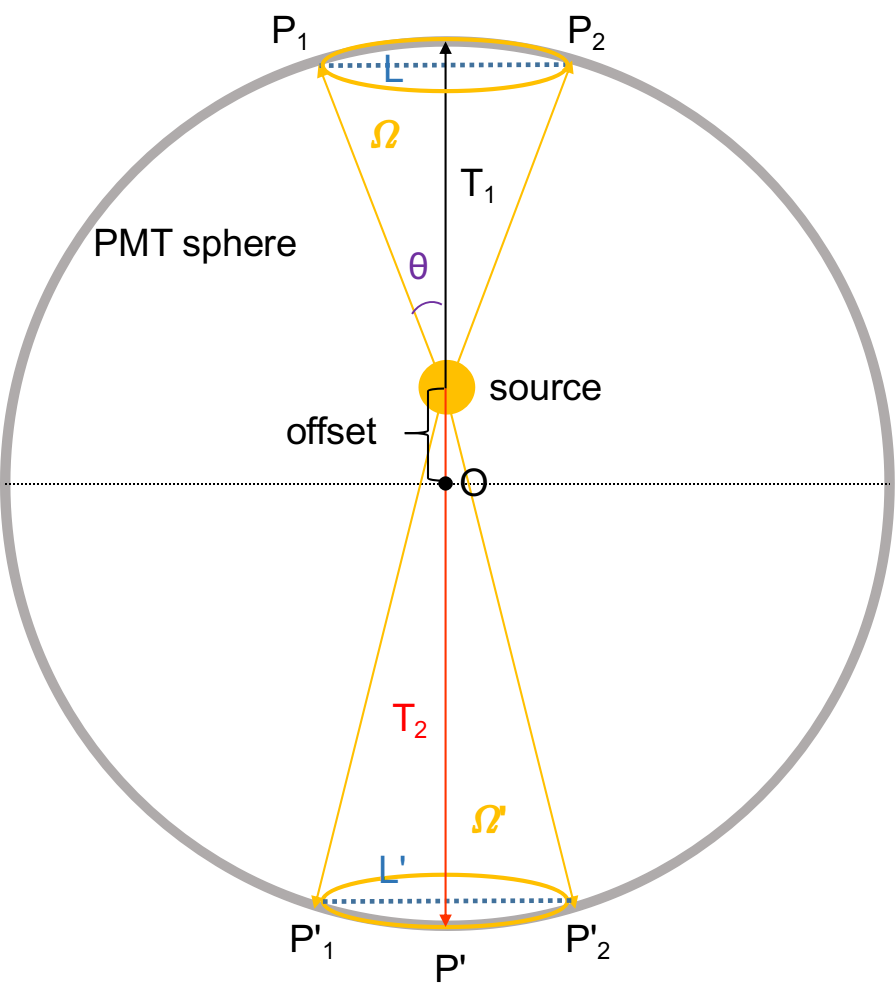
\includegraphics[width=6cm]{n16_groupVelocity.png}
	\caption{$^{16}$N central run for evaluating the average group velocity.}
	\label{fig:n16_groupVeloctiy}
\end{figure}

On the other hand, a solid angle $\Omega'$ is calculated as opposed to the solid angle $\Omega$ subtended at the source position. Similarly, the triggered PMTs within the $\Omega'$ were found and then the arrival time $T_2$ was calculated. An average group velocity was then calculated as:
\begin{equation}
v_\mathrm{gr}=\frac{2 r_\mathrm{PSUP}}{(T_1+T_2)}.
\end{equation}

The final estimate for $v_\mathrm{gr}$ was calculated by averaging the $v_\mathrm{gr}$ values obtained from all the events and triggered PMTs in both run-100934 and run-107055. It was found that $v_\mathrm{gr}=c/n_\mathrm{water,eff}=216.478$ mm/ns, where $n_\mathrm{water,eff}=1.38486$.

The SNO+ collaboration used a more complicated approach to measure actual group velocities in the SNO+ water detector by analyzing a set of laserball calibration runs \cite{anderson2021optical,groupVmeasure}. That analysis can give a more accurate value for $v_\mathrm{gr}$, but it it was not applied here.

For the vertex fitters used in the partial-fill and scintillator phases, since no internal calibration was performed, I adopted the linear interpolation method, which will be discussed in Sect.~\ref{sect:scintFitter}.

\subsection{Fitter Pull and Drive Correction}\label{sect:fitterPull}

An effect of ``fitter pull'' in the event vertex reconstruction utilizing the Cherenkov light was observed in the SNO experiment. The distribution of $(\vec{X}_{fit}-\vec{X}_{MC})/|\vec{X}_{fit}-\vec{X}_{MC}|\cdot \vec{u}_{fit}$ shows a large peak at +1, which indicates that the fitted position $\vec{X}_{fit}$ is prone to be pulled forward from the true position systematically along the event direction$\vec{u}$ \cite{driveCorPeter,brice1996monte,coulter2013modelling}. 

Similar to the SNO heavy water case, in the SNO+ ultrapure water, Cherenkov photons created by an event trigger most of the PMT-hits with early timing and these hits are located within the Cherenkov cone; for the same event, there are also a few PMT-hits with later timing. These later PMT hits can be caused by scattered or reflected photons, and the positions of the hit PMTs are randomly distributed on the PSUP. A random PMT hit is more likely to be placed outside the Cherenkov cone, due to the detector geometry. This can be understood as follows. Consider an event at the center of the PSUP: the Cherenkov cone it produces will intersect the PSUP over an area of $2\pi R^2_\mathrm{PSUP}(1-\cos41^\circ)$, equivalent to about 12\% of the total area of the PSUP sphere. Therefore a random PMT-hit on the PSUP sphere has more than an 88\% likelihood of {\em not} lying within the Cherenkov cone. 

For these later timing PMT hits, a ``complementary'' effect similar to that mentioned in Sect.~\ref{sect:tuneGroupVelocity} can also happen. When the fitter deduces a large $t_\mathrm{res}$ value caused by the later timing hits, it pulls the trial position away from the later timing hits to increase $t_\mathrm{transit}$ and decrease $t_\mathrm{res}$, as illustrated in Fig.~\ref{fitterPull}. In Ref.~\cite{driveCorPeter} this effect was referred to as the ``straightening out of delayed photons'' by the timing fitter. Furthermore, the major early hits can also cause small $t_\mathrm{res}$ values and thus the fitter pulls the trial position closer towards the early hits to decrease $t_\mathrm{transit}$ and increase $t_\mathrm{res}$. Recall that the early hits are located on or around the Cherenkov cone, therefore an overall effect of this ``fitter pull'' is that the fitted position will be pulled along the axis of the Cherenkov cone and towards the PSUP sphere. This pull direction is coincident with the event direction.

\begin{figure}[!htb]
	\centering
	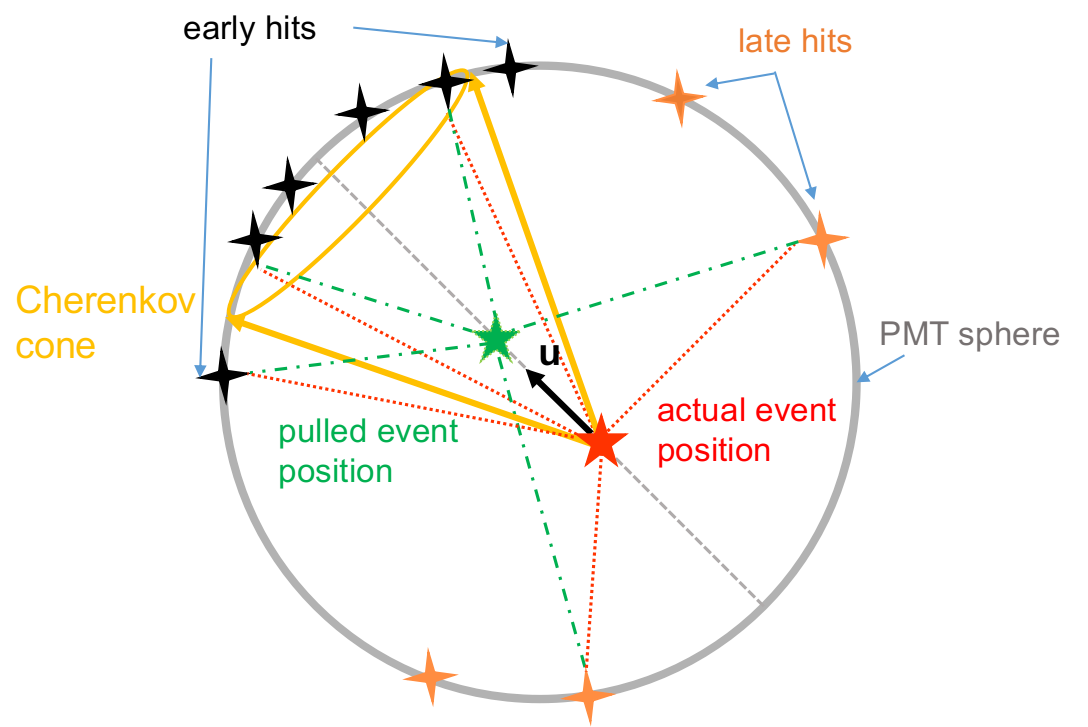
\includegraphics[width=8cm]{fitterPull.png}
\caption[A cartoon shows fitter pull effect.]{This schematic illustrates the fitter pull effect, modified from Fig.~C.2 in Ref.~\cite{brice1996monte} and Fig.~2,3,4 in Ref.~\cite{driveCorPeter}.}
	\label{fitterPull}
\end{figure}

A simple way to eliminate this ``fitter pull'' effect is to pull back the fitted event position against the event direction. This is called ``drive correction''. Once the \texttt{MPW fitter} obtains the fitted position and direction, the drive correction $\vec{X}_{\mathrm{corrected}} = p_0\vec{X}_{fit}+p_1\vec{u}_{fit}$ is applied on the fitted position, where $p_0$ and $p_1$ are the correction parameters (see Fig.~\ref{drivecor}).
\begin{figure}[!htb]
	\centering
	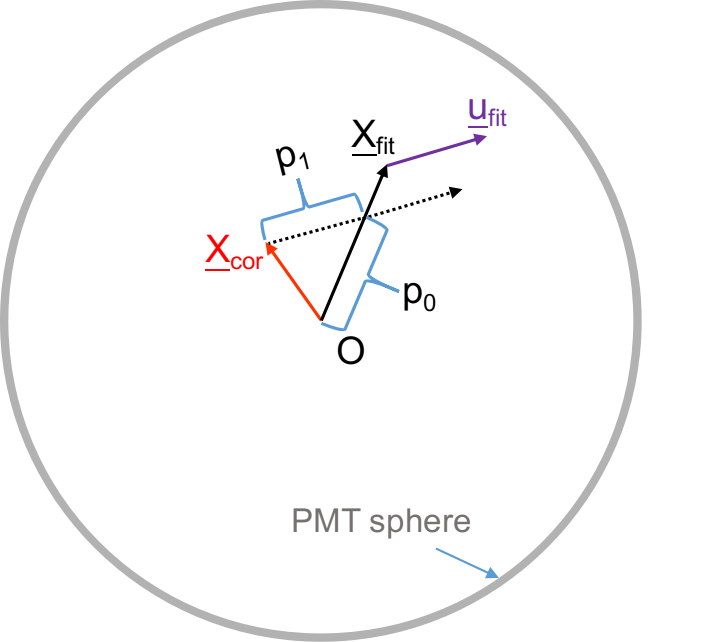
\includegraphics[width=6cm]{driveCor.png}
	\caption{ A diagram illustrating the drive correction.}
	\label{drivecor}
\end{figure}

To obtain the values of $p_0$ and $p_1$, I generated electron events uniformly distributed inside the AV, with energies ranging from 2 to 10 MeV with a 1 MeV step. The \texttt{MPW fitter} was applied on each simulation and returned $\vec{X}_{fit}$ and $\vec{u}_{fit}$. Taking the Monte Carlo generated positions $\vec{X}_{MC}$ as the true positions, for all the fitted events, a $\chi^2$ function was calculated as:
\begin{equation}
\chi^2 = \sum_{i=1}^{N_{\mathrm{events}}}[\vec{X}^i_{MC}-(p_0\vec{X}^i_{fit}+p_1\vec{u}^i_{fit})]^2 \; ,
\end{equation}
and the parameters ($p_0$, $p_1$) were obtained by minimizing the $\chi^2$ function. When calculating $\chi^2$, fitted events having $|\vec{X}_{fit}-\vec{X}_{MC}| > 3~\mathrm{m}$ were rejected to improve the $\chi^2$ minimization results.

For the 2 to 10 MeV $e^-$ event simulations (using \texttt{RAT} version 6.17.6), the values obtained for ($p_0$, $p_1$) are energy- (or NHit-) dependent. However using NHits-dependent functions $p_0(\mathrm{NHit}), p_1(\mathrm{NHit})$ as drive corrections does not improve the results. 
Finally we take average values from the 5 to 10 MeV electron simulations and find the optimal drive correction is: 
\begin{equation}
\vec{X}_{\mathrm{corrected}} = 0.9868\vec{X}_{fit} \, - \, 78.417\vec{u}_{fit}~\mathrm{[mm]} .
\end{equation}

Note that these drive correction parameters were obtained from simulations, and so changes of the simulation model, and especially changes to the optical model of the detector, can affect the $n_{gr,eff}$, mode cut and time residual cut, and thereby affect the drive correction parameters. If needed however the drive correction parameters can be re-coordinated with the changes in the simulation.

\begin{figure}[!htb]
	\centering
	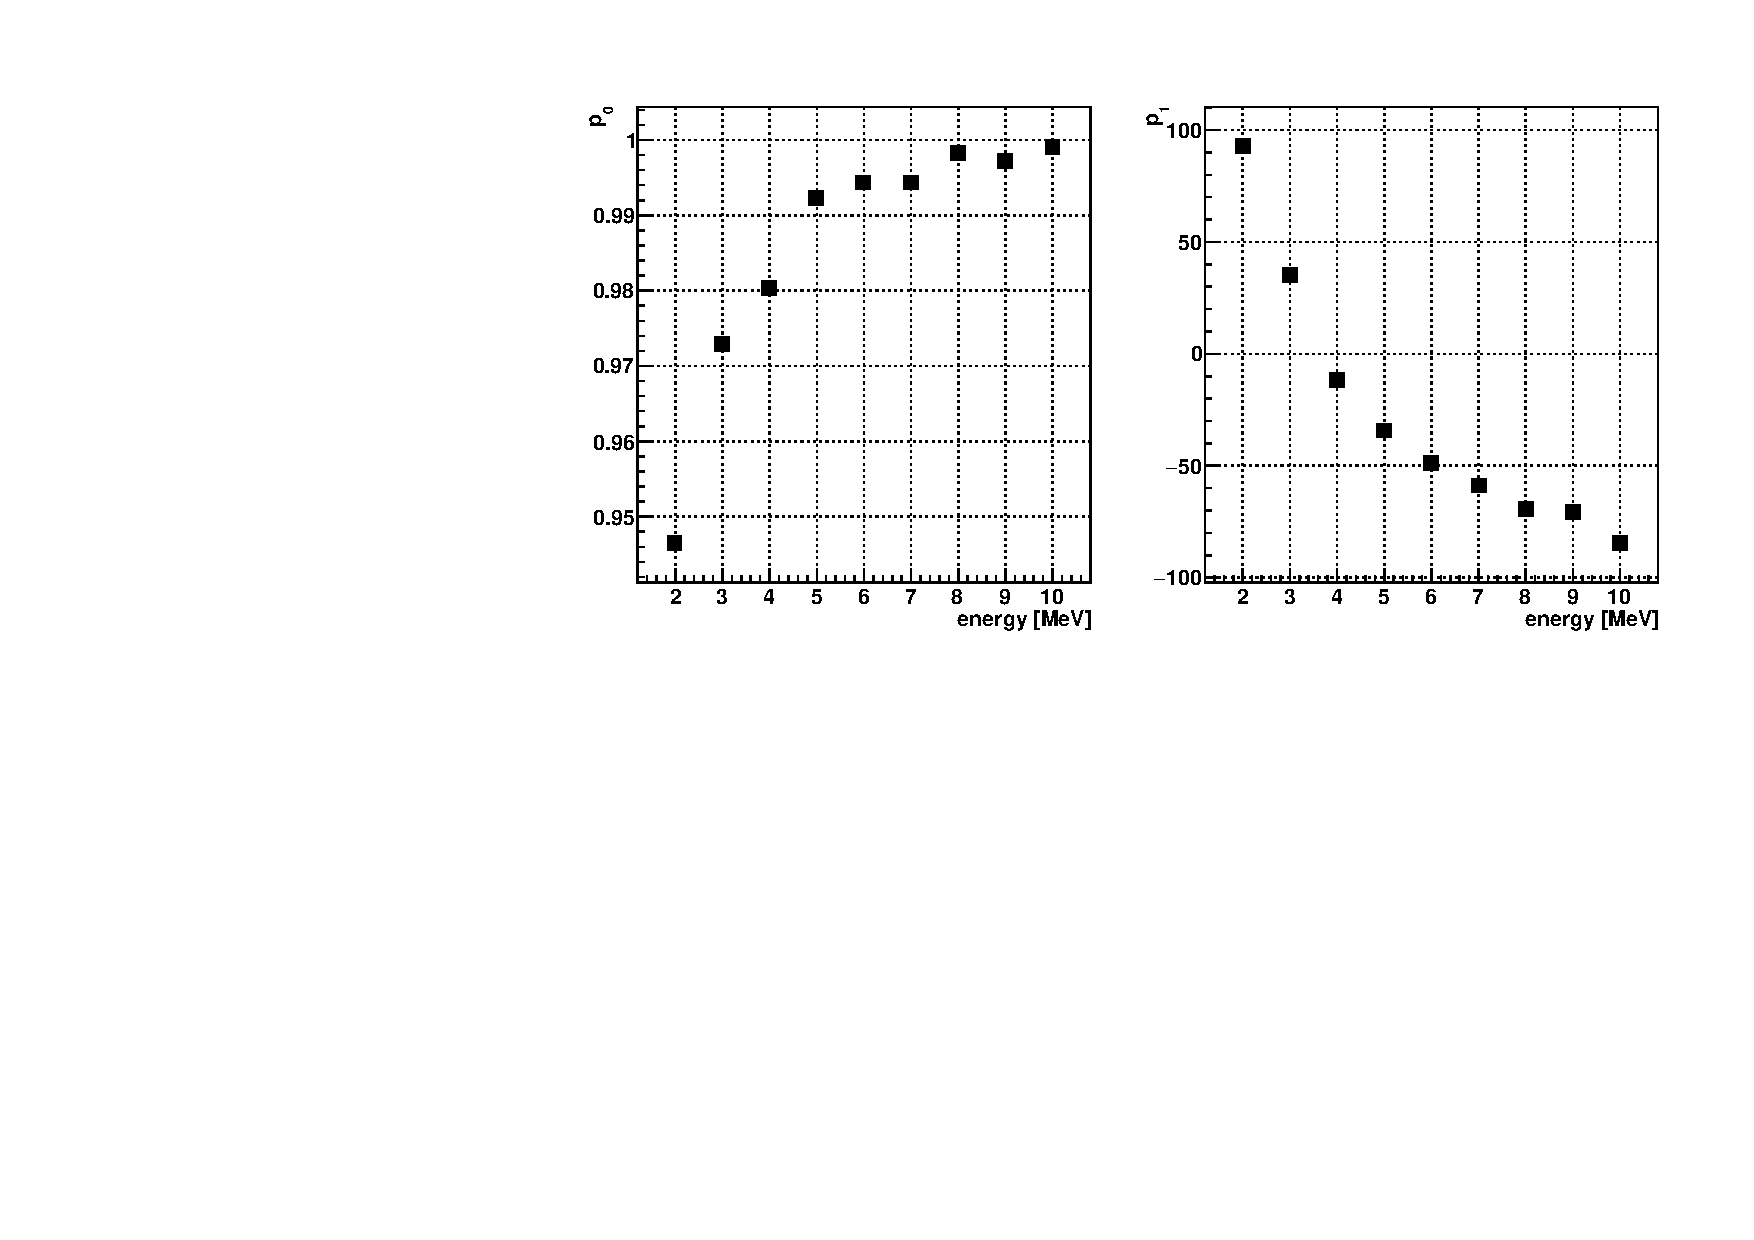
\includegraphics[width=10cm]{pullParVsEnergy.pdf}
	\caption{Drive correction parameter $p_0$ (left) and $p_1$ (right) as a function of electron energy.}
	\label{pullParVsEnergy}
\end{figure}

To check the effects of the drive correction, 1000 simulations of 5 MeV electrons were generated at the detector center, with their momentum vector oriented along $(1,0,0)$. It was found that the drive effect in the reconstruction caused about +50 mm bias away from the detector center and along the $x$-axis (i.e., the pull lay along positive $x$). The drive correction reduced this pull down to about +0.2 mm along the $x$-axis. The resolution of the $r_\mathrm{bias}$ distribution was also improved by $\sim$20 mm. With the same simulation settings, various electron energies from 2 to 10 MeV (with a 1 MeV step) were generated to check the effects before and after the drive correction, with the outcome shown in Fig.~\ref{drivecorVsEnergy}. The pull is quantified by the radial bias mentioned in Sect.~\ref{sect:tuneGroupVelocity}. The distributions of the $r_\mathrm{bias}$ in each simulation were fitted with Gaussian functions, and the Gaussian means were used as the pull. It can be seen that the pull effect is larger at higher electron energy. The drive corrections improve the radial biases by about 55 mm. The drive correction is also applied in the \texttt{Rat water fitter}, and those results are also shown.
\begin{figure}[!htb]
	\centering
	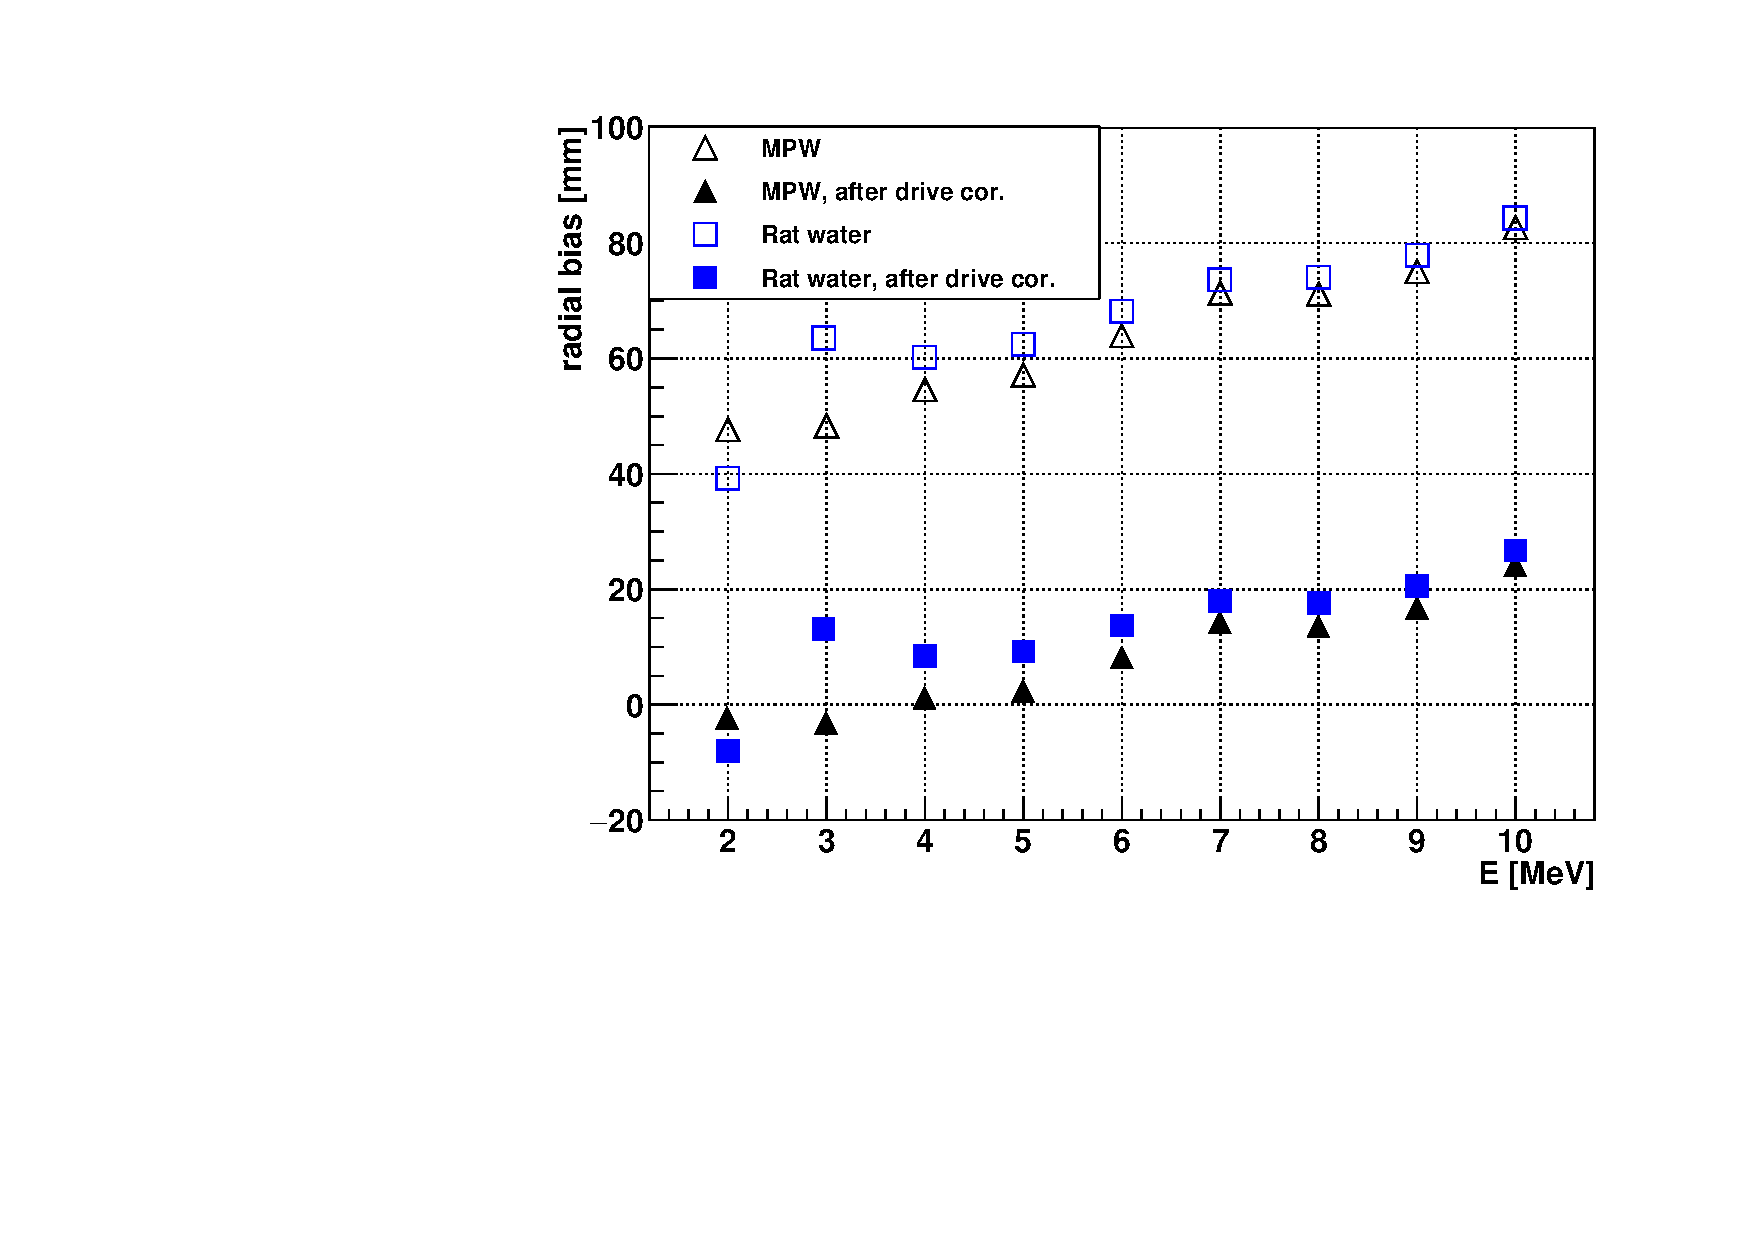
\includegraphics[width=9cm]{pullEffectVsEnergy.pdf}
	\caption[Radial biases of simulated electron events as a function of energy.]{Radial biases of simulated electron events before (unfilled triangles) and after the application of a drive correction (filled triangles), as a function of energy. The results from the official \texttt{RAT water fitter} are also shown, with the unfilled blue squares for biases before the correction and filled blue square after the correction.}
	\label{drivecorVsEnergy}
\end{figure}

\subsection{PMT Selectors for the Reconstruction}\label{sect:PMTselector}

PMT selectors were developed to optimally select a set of hit PMTs for the reconstruction algorithm, from all the PMTs triggered by an event. The purpose was to optimize the fitter results and boost the fit speed. The PMT selectors used by the \texttt{MP fitter} are:

\begin{itemize}
	\item[$\bullet$] Straight Light Path Time Residual Cut Selector
	
	This selector is used for the direction reconstruction for the SNO+ water phase, and was first developed by K. Singh \cite{kalpanaMPFitter}. The time residual ($t_\mathrm{res}$) is calculated for each hit PMT, and PMTs returning a $t_\mathrm{res}$ value within the prompt time window $[-10.0, 120.0]$ ns are selected for the fitter. The calculation of $t_\mathrm{res}$ is based on using straight line light paths, as in the case of the \texttt{MPW fitter}. The selector mostly removes PMTs that had been triggered by late arriving photons, such as those reflected off the detector elements (called ``late light''), and thereby keeps the possible Cherenkov ring hit pattern clear for the direction reconstruction. Removing irrelevant PMTs can potentially boost the fit speed.
	
	\item[$\bullet$] Mode Cut Selector
	
	This selector was developed by the SNO+ collaboration for all fitters. It checks the hit time ($t_\mathrm{PMT}$) distributions of all the hit PMTs and finds the mode of the hit time ($t_\mathrm{mode}$). Here the $t_\mathrm{mode}$ is required to be a unique number and is found by looking for the peak of the $t_\mathrm{PMT}$ distribution. If it fails to get $t_\mathrm{mode}$, it instead calculates the median ($t_\mathrm{median}$) \cite{modeCut}. Then it selects PMTs for which $t_\mathrm{PMT} \in [t_\mathrm{mode}+t_\mathrm{low}, t_\mathrm{mode}+t_\mathrm{high}]$ ns. This selector is used to remove the PMTs triggered by noise, or reflected light. The values of $t_\mathrm{low}$ and $t_\mathrm{high}$ are optimized for different detection media. For the \texttt{MPW fitter}, the optimized window is found to be $[t_\mathrm{mode}-50, t_\mathrm{mode}+100]$ ns by checking with the fit biases and resolutions for the $^{16}$N central run data in the water phase, while for the \texttt{MP partial fitter} and \texttt{MP scint fitter}, the optimized window is $[t_\mathrm{mode}-100, t_\mathrm{mode}+100]$ ns based on tuning with the simulations.
	
	\item[$\bullet$] Uniform PMT Selector
	
	I implemented this selector and the Earliest Hit Selector mentioned below for the partial-fill and scintillator phases, when a single event can trigger many PMTs due to the high light yields of the liquid scintillator. In this case, the fit speed for each event becomes slow, which can present a difficulty for the data processing. These selectors can reduce the number of the hit PMTs to a designated number ($n_\mathrm{select}$) to boost the fit speed, while still providing acceptable values for fit bias and resolution. 
	
	For the Uniform PMT Selector, when an event triggers $N$ calibrated PMTs, the selector goes through these recorded PMTs and uniformly picks one PMT per interval of $\left \lceil{N/n_\mathrm{select}}\right \rceil $. If $N\leq n_\mathrm{select}$, the selector does nothing. In this way the selector uniformly reduces the number of the PMTs for the fitter, without introducing an obvious bias.
	
	\item[$\bullet$] Earliest Hit PMT Selector
	
	This selector first groups the PMTs by their positions on the PSUP sphere. Taking the centre of the sphere as the origin of the coordinate, the sphere is decomposed into intervals of azimuth angle $\phi$ (longitude) and zenith angle $\theta$ (latitude). The PMT positions are projected to $\phi\in [-\pi,\pi]$ and $\cos\theta\in [-1, 1]$ on the sphere, each range being uniformly divided into $n$ intervals. Thus, the PMTs are grouped into $n\times n$ panels by $\phi$ and $\cos\theta$: $\mathrm{PMT}(\phi_i,\cos\theta_j) \in [i\cdot\phi/n, j\cdot\cos\theta/n],~(i,j=1,2,..,n)$, see Fig.~\ref{GroupPMTs}. 
	\begin{figure}[!htb]
		\centering
		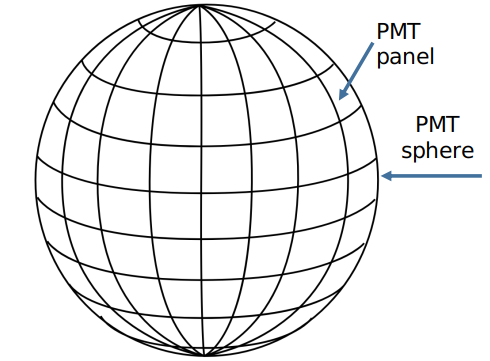
\includegraphics[width=5cm]{GroupPMTs.png}
		\caption{PMTs are grouped by partitioning the PSUP sphere into intervals of latitude and longitude.}
		\label{GroupPMTs}
	\end{figure}
	
	In each panel, the selector first removes the hit PMTs which are triggered too early ($t_\mathrm{PMT}<100$ ns, where 100 ns is set as a default threshold). These PMTs could be triggered by noises, such as the pre-pulsing from thermal noises. Then in the rest of the hit PMTs, the selector picks up one PMT which has the earliest $t_\mathrm{PMT}$ in the panel. Thus the number of the hit PMTs is reduced to $n\times n$ for the fitter, i.e., $n_\mathrm{select}=n\times n$. If $\mathrm{NHits}\leq n_\mathrm{select}$, the selector does nothing. 
	
		Other timing parameters can also be used for selecting the PMT in each panel, such as $t_\mathrm{mode}$ or $t_\mathrm{median}$. However, tests on the simulations for the scintillator phase showed that using the earliest hit time $t_\mathrm{PMT}$ gave smaller fit bias and better fit resolution. Tests on the 10 MeV $e^-$ simulations in the scintillator phase showed that by applying this selector with $n_\mathrm{select}=16\times16$, the fit speed was reduced from 1.2 s/event to 0.4 s/event.
\end{itemize}

\subsection{Position Figure of Merit}\label{sect:positionFoM}

A quantity called scaled $\log L$ ($scaleLogL$) is used as the position reconstruction figure of merit ($posFoM$): $scaleLogL = \ln L/\mathrm{NHit}_\mathrm{selected}$. This quantity utilizes the best log-likelihood returned by the \texttt{MP fitter} for a successfully reconstructed event vertex, and then it is scaled by the ``selected'' NHits ($\mathrm{NHits}_\mathrm{selected}$), which is the number of the PMTs actually used by the fitter for the event vertex reconstruction, after the PMT selection mentioned in Sect.~\ref{sect:PMTselector}. This $posFoM$ quantity can remove a few mis-reconstruct events and thereby improve the results of the reconstruction.

\subsection{Performance of the Water Vertex Reconstruction}\label{sect:waterFitterVertex}

Using the \texttt{RAT} (version 6.17.6) package, MC simulations were performed in which 10,000 electron events were generated at the detector center (in the PSUP coordinate frame) with isotropic direction, i.e. the orientation of the momentum vector was generated randomly and uniformly over the entire solid angle ($4\pi$). The default detector trigger settings of the SNO+ water phase were \texttt{N100Hi}=21.0, \texttt{N100Med}=16.0 and \texttt{N100Lo}=11.0 and with those settings some events, especially those with lower energies ($E<3$ MeV), may fail to trigger the detector. Since the fitters only reconstruct triggered events, the number of events reconstructed by the fitter may be lower than the number simulated.

The average fit speed of the event vertex reconstruction for the 5 MeV $e^-$ simulations was 0.005 s/event and for the direction reconstruction fit speed was 0.002 second/event, figures that are very fast and certainly acceptable for the data processing in the SNO+ water phase. Fig.~\ref{fig:5MeVbeta_center_water} shows the position reconstruction results and performance for the 5 MeV $e^-$ events. The bias between the fitted and MC positions, $\vec{X}_{fit}-\vec{X}_{mc}=(x_{fit}-x_{MC},y_{fit}-y_{MC},z_{fit}-z_{MC})$, was projected onto the $(x,y,z)$ axes respectively and its distribution was fitted with Gaussian functions. The mean of the fitted Gaussian ($\mu$) is taken as the fit position bias while the standard deviation ($\sigma$) is taken as the fit position resolution.
\begin{figure}[htbp]
	\centering 
	\subfigure[$x_{fit}-x_{mc}$]{
		\begin{minipage}[t]{0.5\textwidth}
			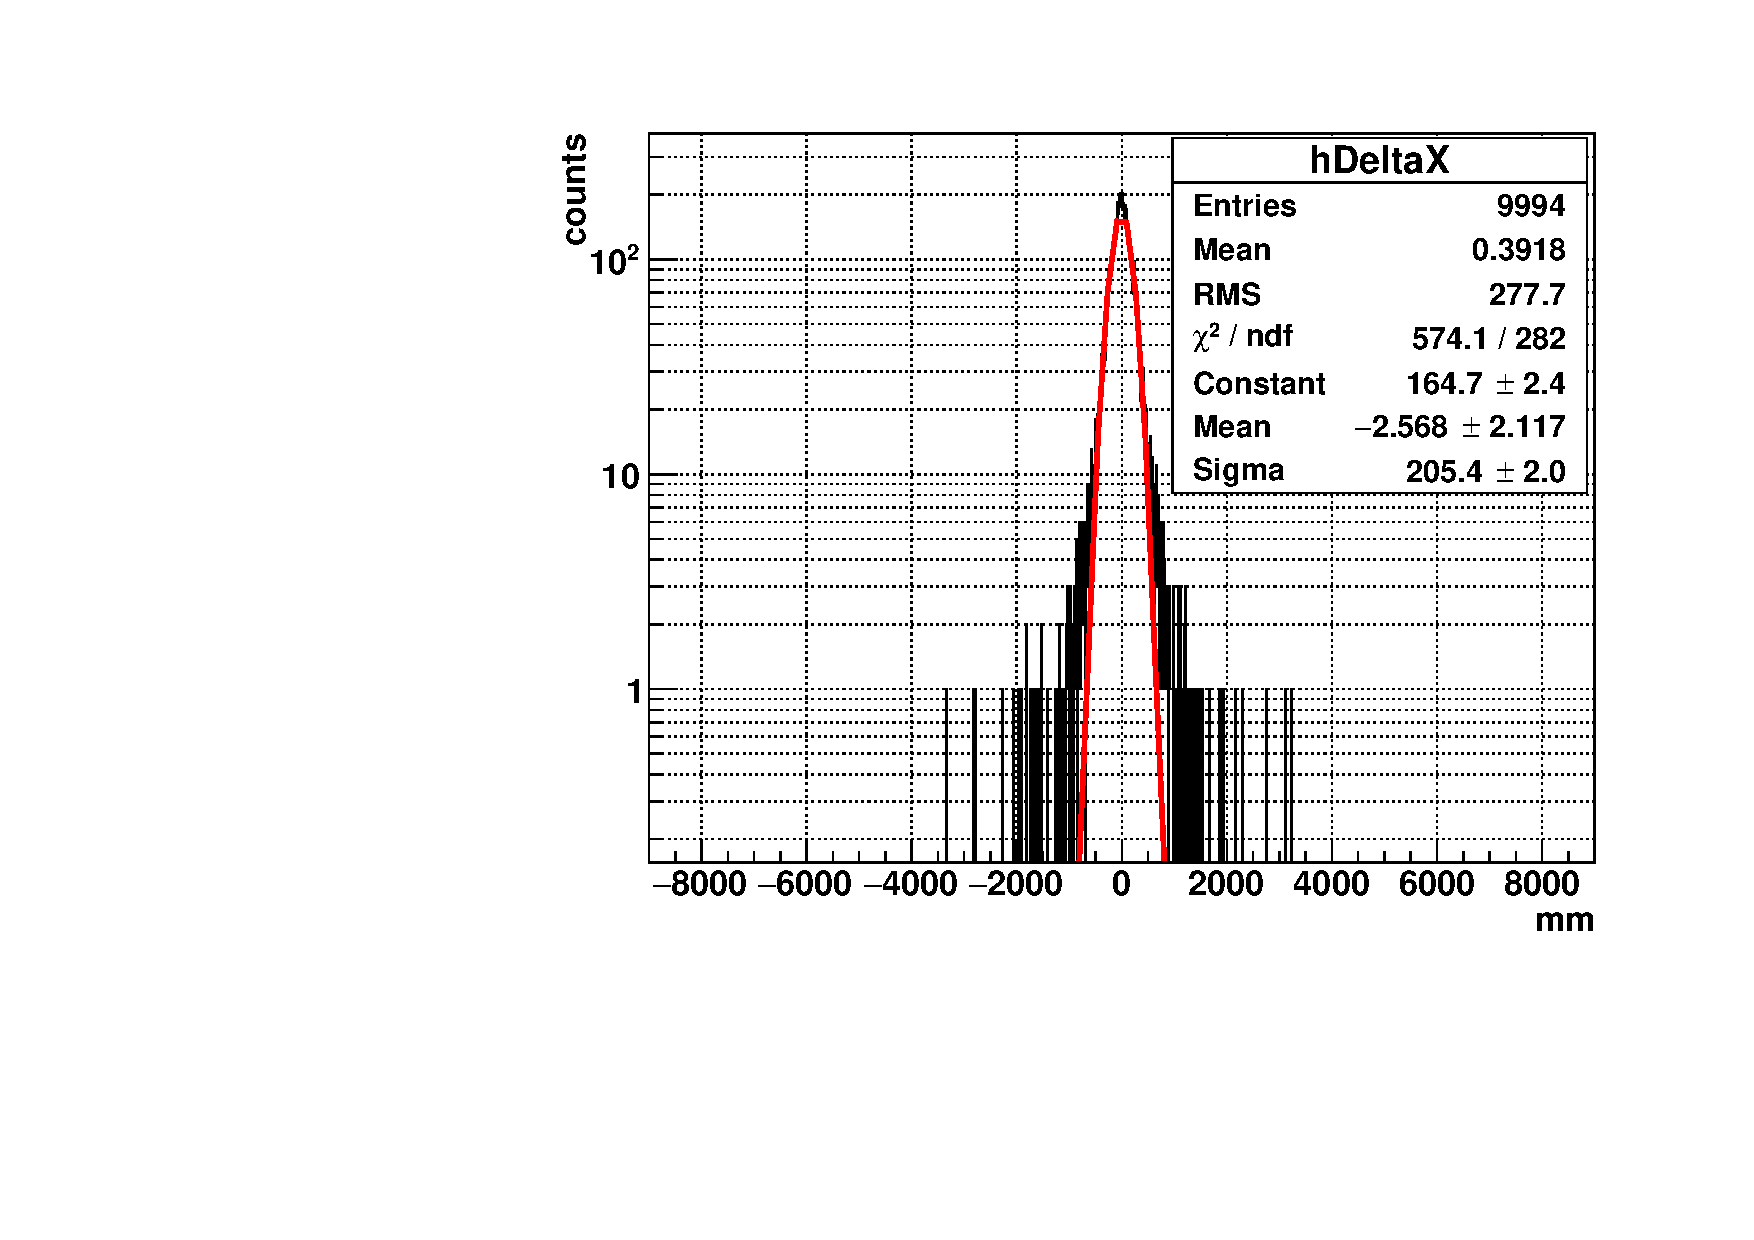
\includegraphics[width=8cm]{5MeVbetaX.pdf}
		\end{minipage}
	}
	\subfigure[$y_{fit}-y_{mc}$]{ 
		\begin{minipage}[t]{0.4\textwidth}
			\centering
			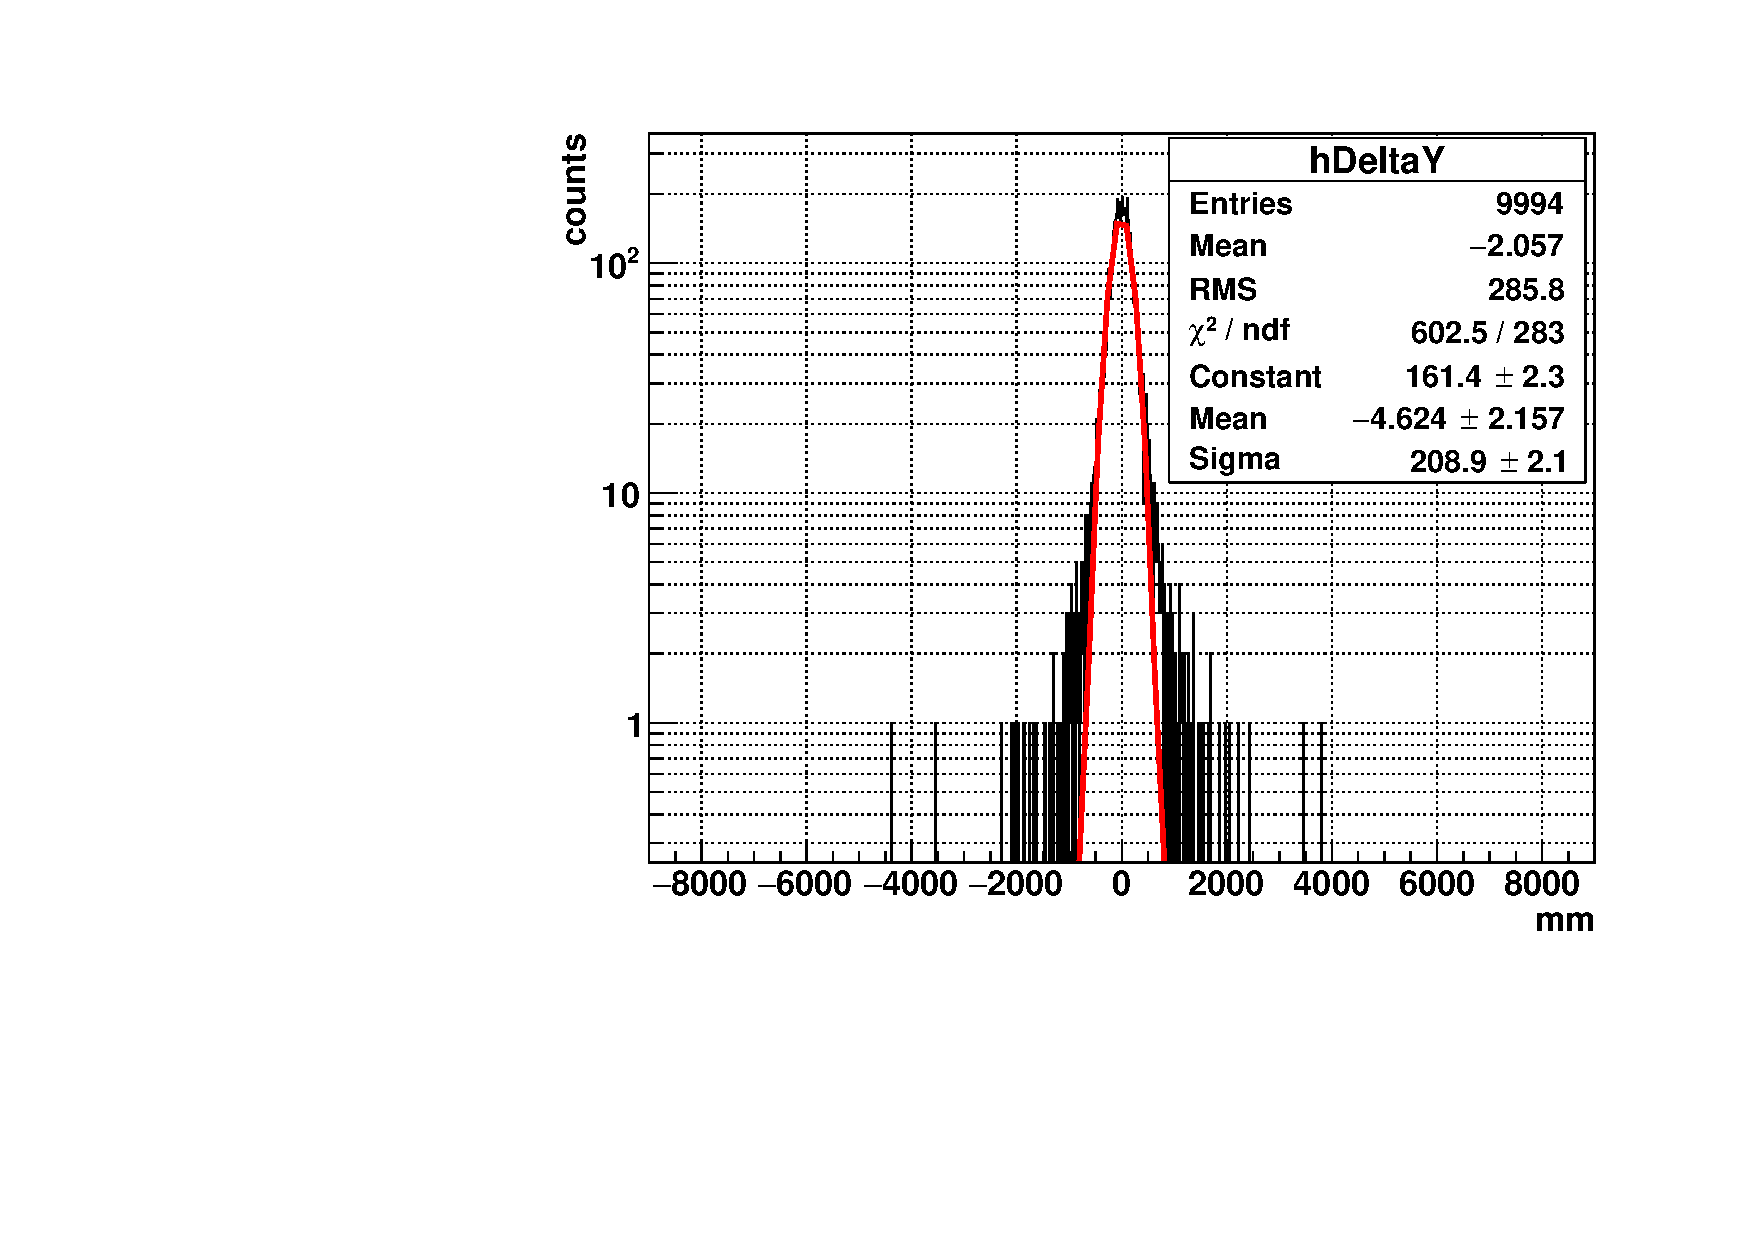
\includegraphics[width=8cm]{5MeVbetaY.pdf}
		\end{minipage}
	}
	\subfigure[$z_{fit}-z_{mc}$]{ 
		\begin{minipage}[b]{0.4\textwidth}
			\centering
			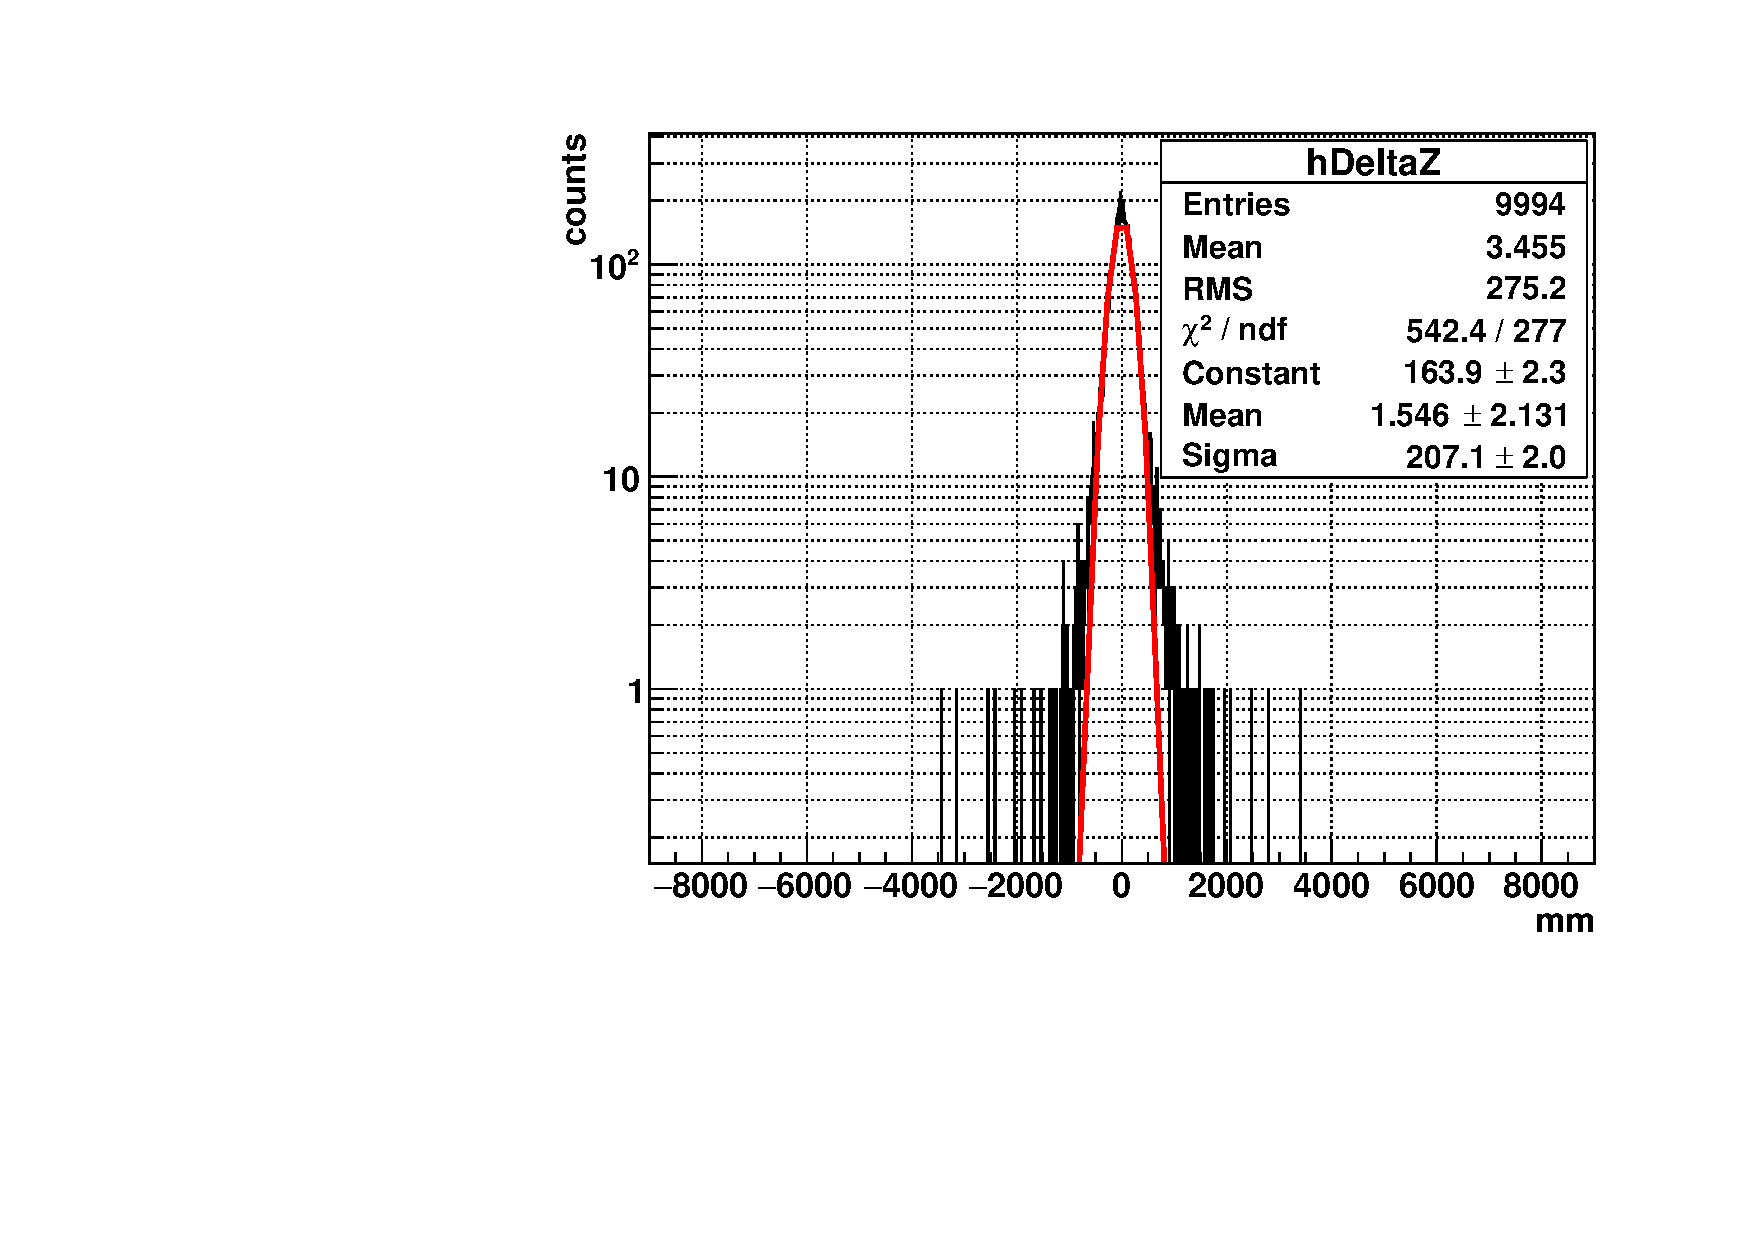
\includegraphics[width=8cm]{5MeVbetaZ.pdf}
		\end{minipage}
	}
	\caption[The position biases projected on the x, y and z axes.]{The position biases projected on the x, y and z axes. The distributions were fitted with Gaussian functions. The MC generated 10000 5-MeV $e^-$ particles at the detector center with isotropic directions.\label{fig:5MeVbeta_center_water}}
\end{figure}

In Fig.~\ref{fig:5MeVbeta_center_water} there are a few events with position biases larger than 2000 mm, and these are interpreted as being mis-reconstructed events. Some of these events are due to relatively lower log-likelihood values and can be tagged by the $posFoM$ mentioned in Sect.~\ref{sect:positionFoM}. As shown in Fig.~\ref{fig:posFOM_5MeVbeta_center_water}, a cut requiring $scaleLogL>10$ can remove some mis-reconstructed events. The remainder may have resulted from the `straight light path' approximation used by the \texttt{MP fitter}, since this calculation misrepresents refracted and/or reflected light paths from event to PMT, as mentioned in Sect.~\ref{sect:waterVertex}. However, the fraction of these mis-reconstructed events is low, about 0.1\% and thus it is tolerable.

\begin{figure}[htbp]
	\centering 
	\subfigure[$x_{fit}-x_{mc}$ vs. $scaleLogL$.]{
		\begin{minipage}[t]{0.5\textwidth}
			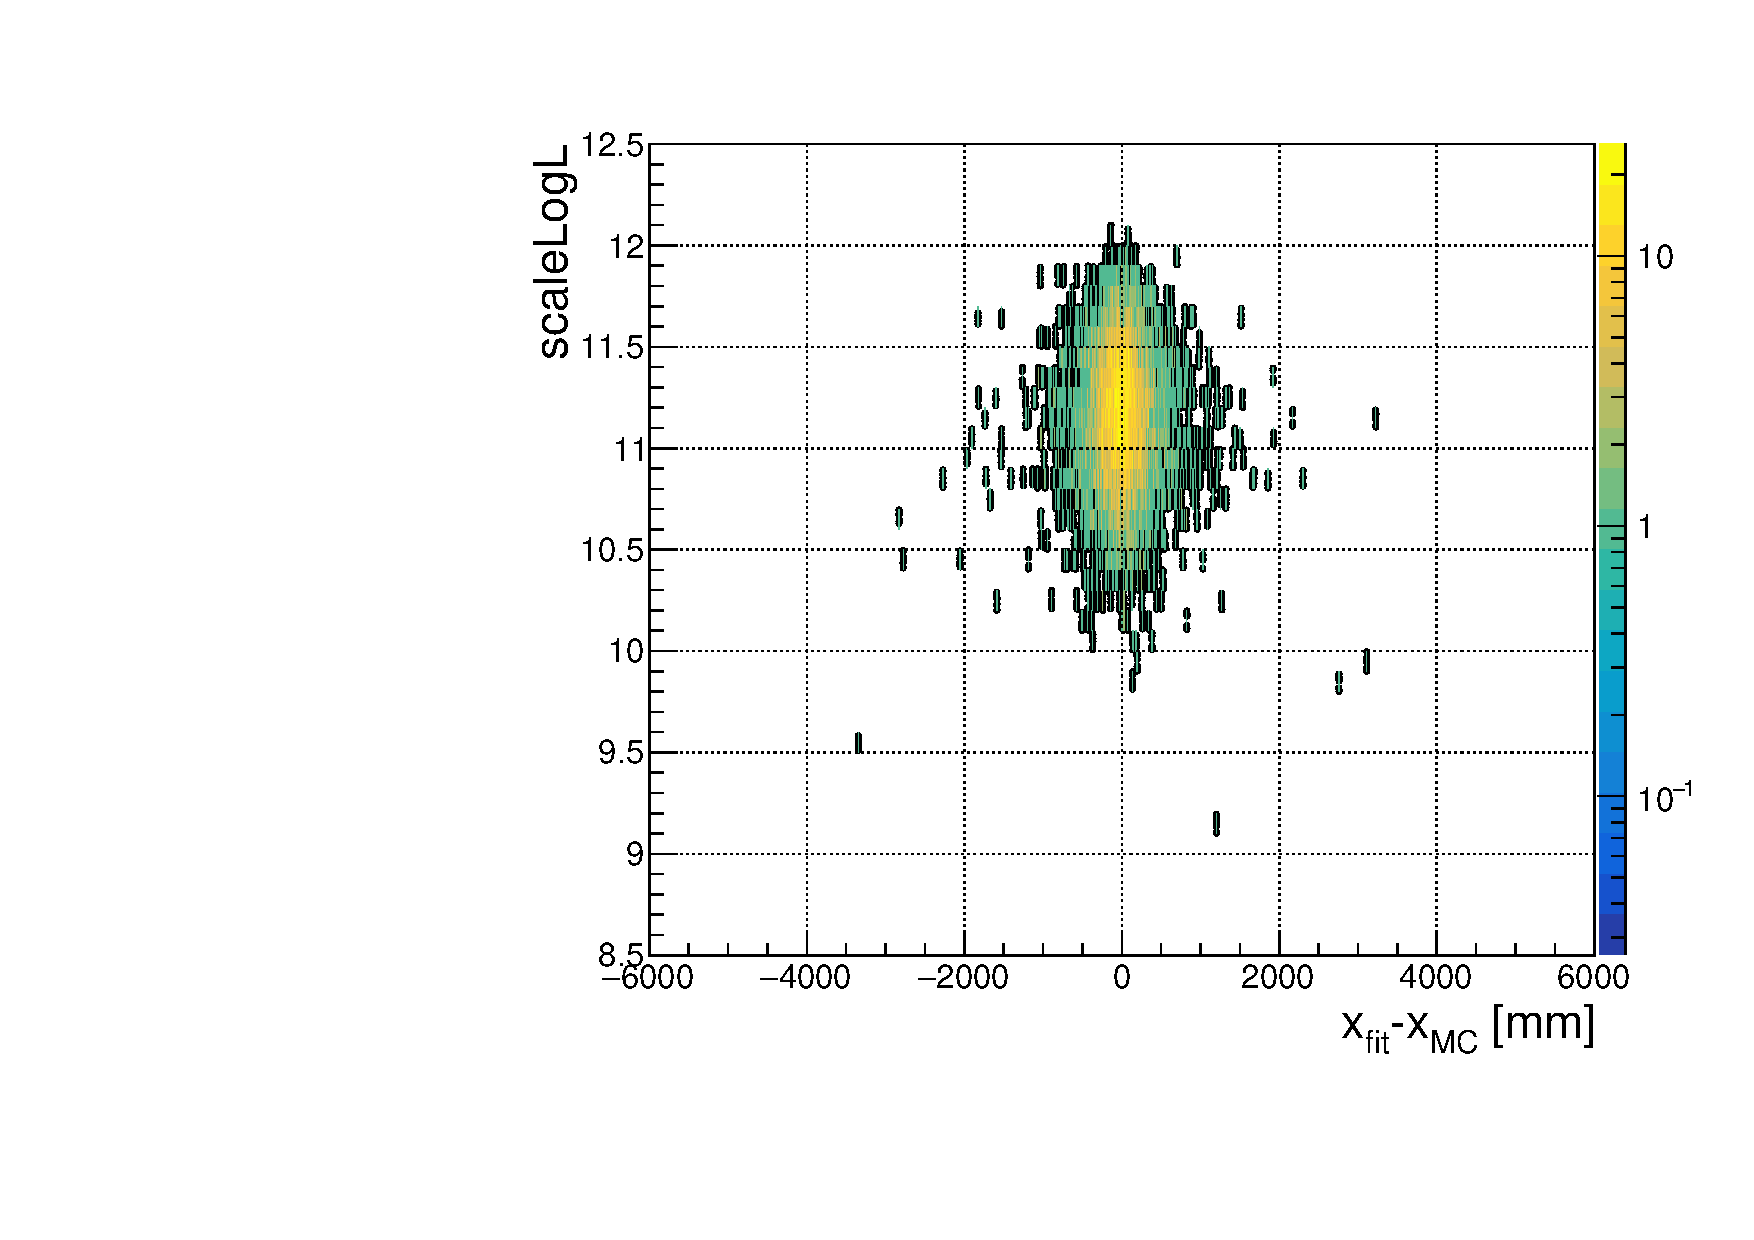
\includegraphics[width=8cm]{scaleLogLvsX_water5MeV.pdf}
		\end{minipage}
	}
	\subfigure[$y_{fit}-y_{mc}$ vs. $scaleLogL$.]{ 
		\begin{minipage}[t]{0.4\textwidth}
			\centering
			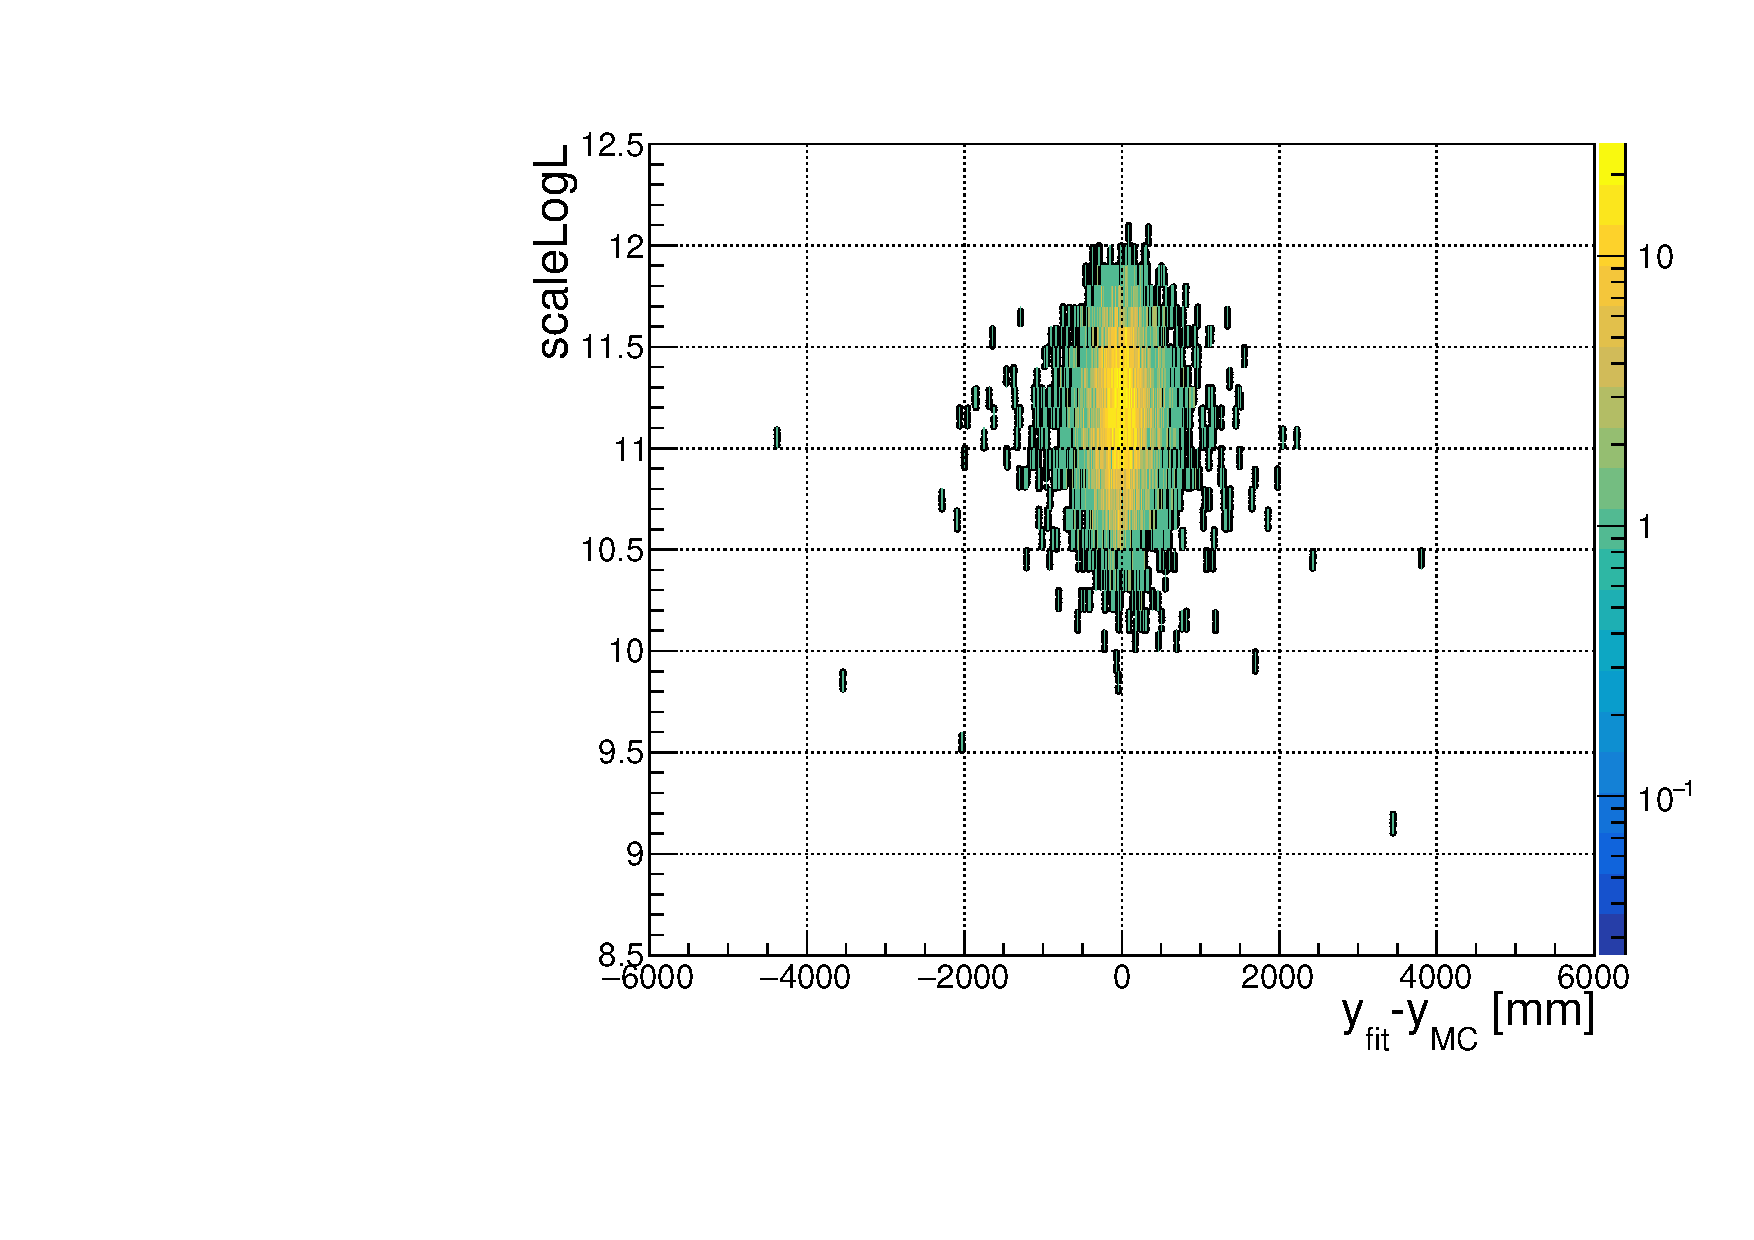
\includegraphics[width=8cm]{scaleLogLvsY_water5MeV.pdf}
		\end{minipage}
	}
	\subfigure[$z_{fit}-z_{mc}$ vs. $scaleLogL$.]{ 
		\begin{minipage}[b]{0.4\textwidth}
			\centering
			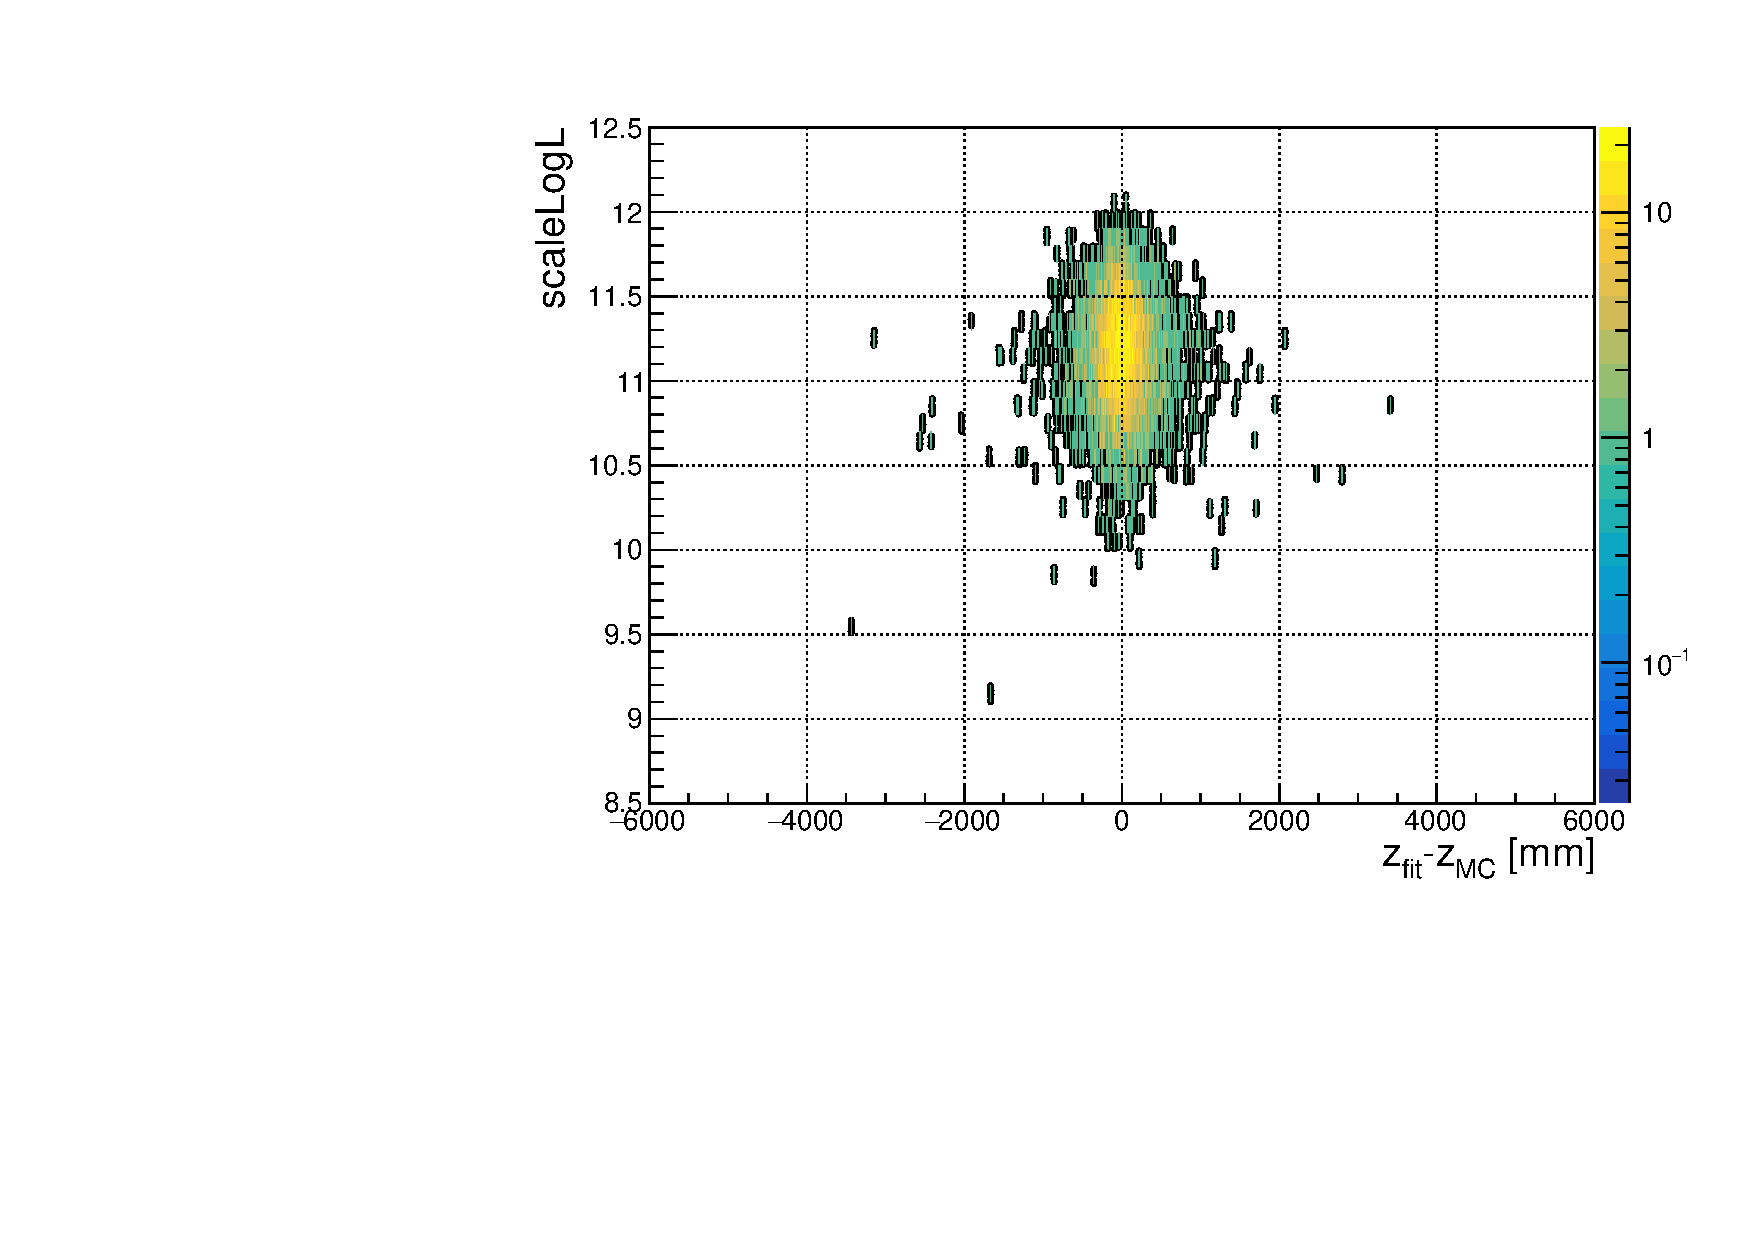
\includegraphics[width=8cm]{scaleLogLvsZ_water5MeV.pdf}
		\end{minipage}
	}
	\caption[The position biases against the position FoMs.]{The position biases against the position FoMs. The MC generated 10000 5-MeV $e^-$ particles at the detector center with isotropic directions.\label{fig:posFOM_5MeVbeta_center_water}}
\end{figure}

The above results pertain to electron events at the centre of the PSUP, but a more realistic analysis must permit events to happen anywhere and everywhere inside the AV. To simulate this, electron events were generated at random positions uniformly distributed inside the AV volume, and (again) with isotropic directions. Simulations were performed for a range of $e^-$ energies covering 2 to 15 MeV, with a 1 MeV interval. Fig.~\ref{fig:MPWposBias_isoFill} and Fig.~\ref{fig:MPWposResol_isoFill} show the fit position bias ($\mu_{x,y,z}$) and resolution ($\sigma_{x,y,z}$) respectively. 

These results show that the fit position biases $\mu_{x,y,z}$ are stable across different energies and (with two exceptions) smaller than 10 mm in magnitude. The resolution $\sigma_{x,y,z}$ improve (i.e. the $\sigma$'s decrease) with increasing event energy, from about 350 mm at 2 MeV to about 120 mm at 15 MeV, the average value being 180 mm. Of course more photons are produced by higher-energy $e^-$ events, thus triggering more PMTs, and events having a larger NHits value provide more information for the fitter: this explains the trend in resolution given by Fig.~\ref{fig:MPWposResol_isoFill}. As will be shown in the following section, the position resolution can also be improved by using a detection medium that produces more photons for the same event. 

\begin{figure}[htbp]
	\centering	
	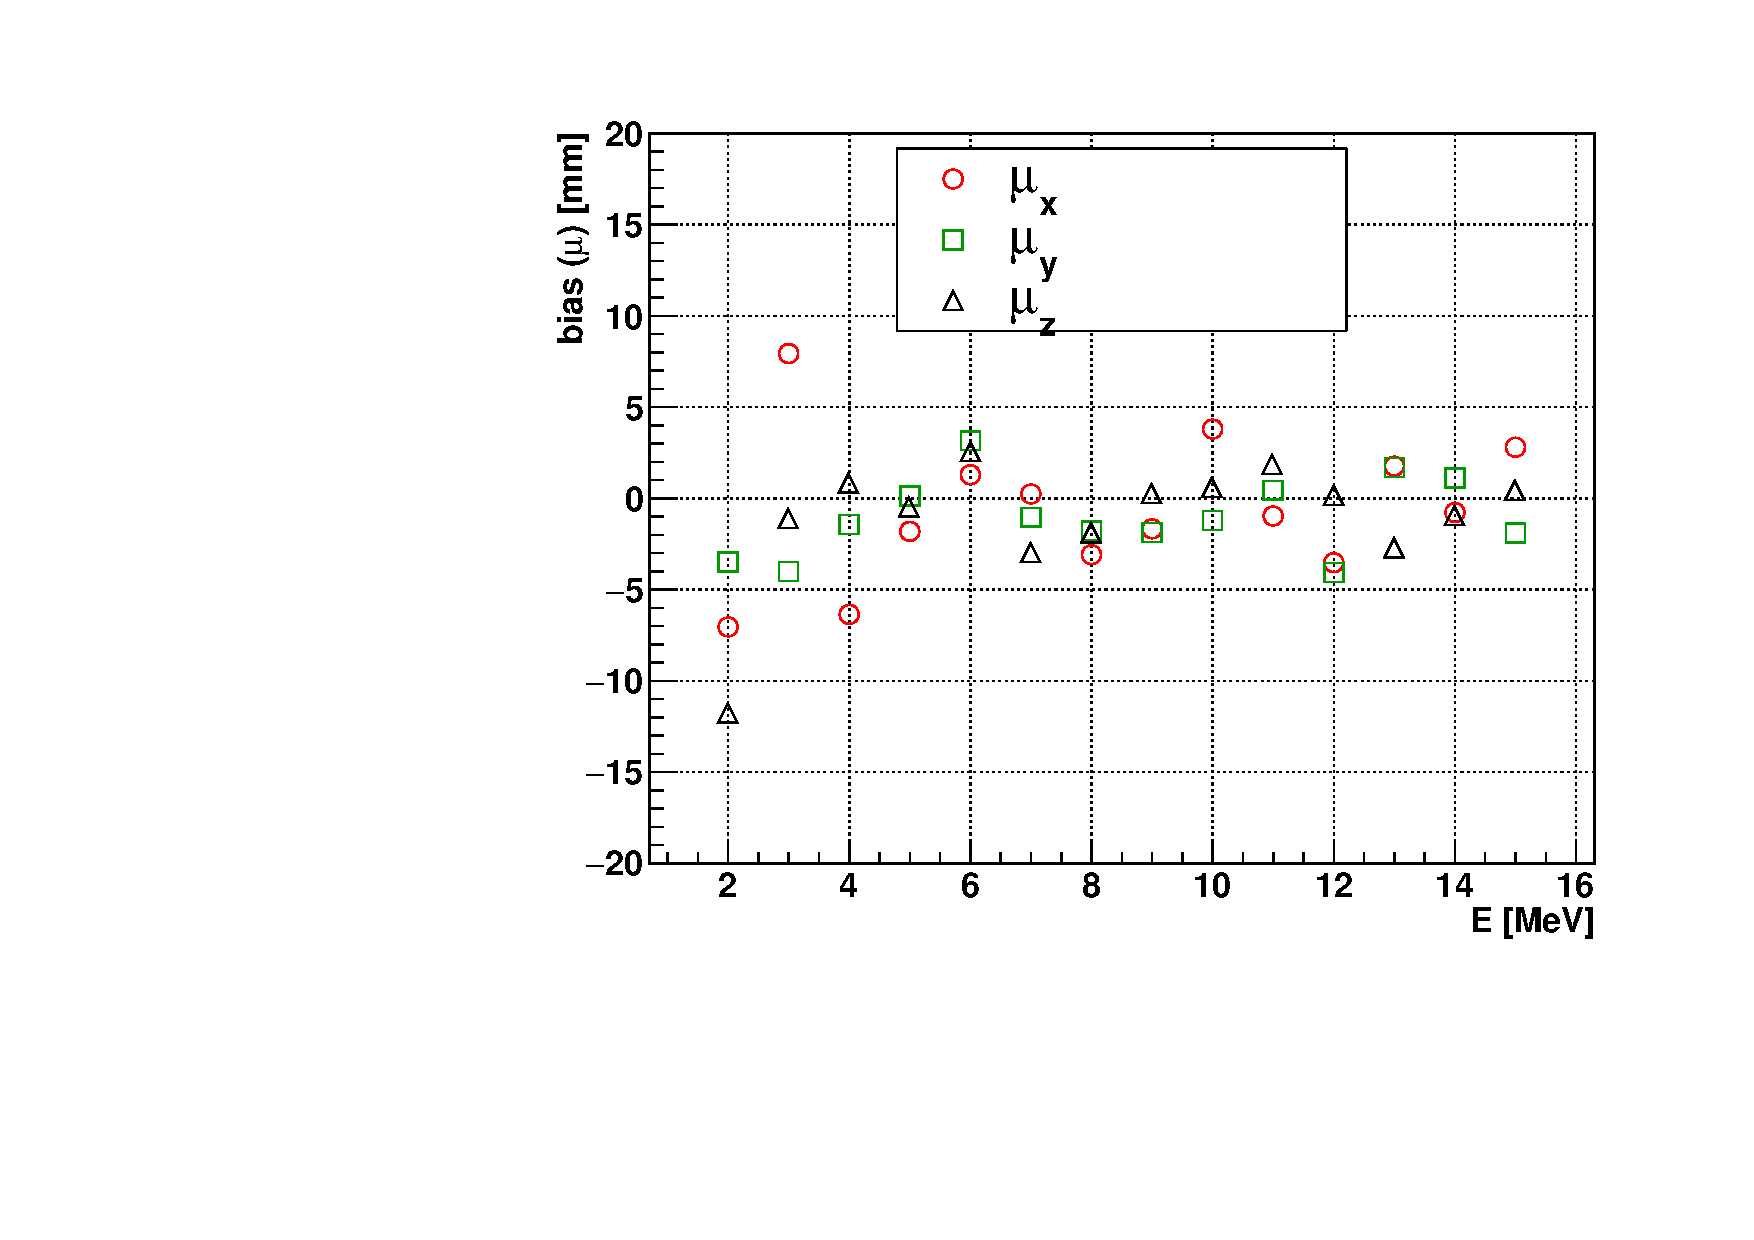
\includegraphics[width=9cm]{MPW_isoFill_posBiasVsE.pdf}
	\caption[The \texttt{MPW fitter} fit position biases ($\mu_{x,y,z}$) as a function of energy.]{The \texttt{MPW fitter} fit position biases in x(red circle), y (green square), and z (black triangle) axes as a function of energy. \label{fig:MPWposBias_isoFill}}
\end{figure}

\begin{figure}[htbp]
	\centering	
	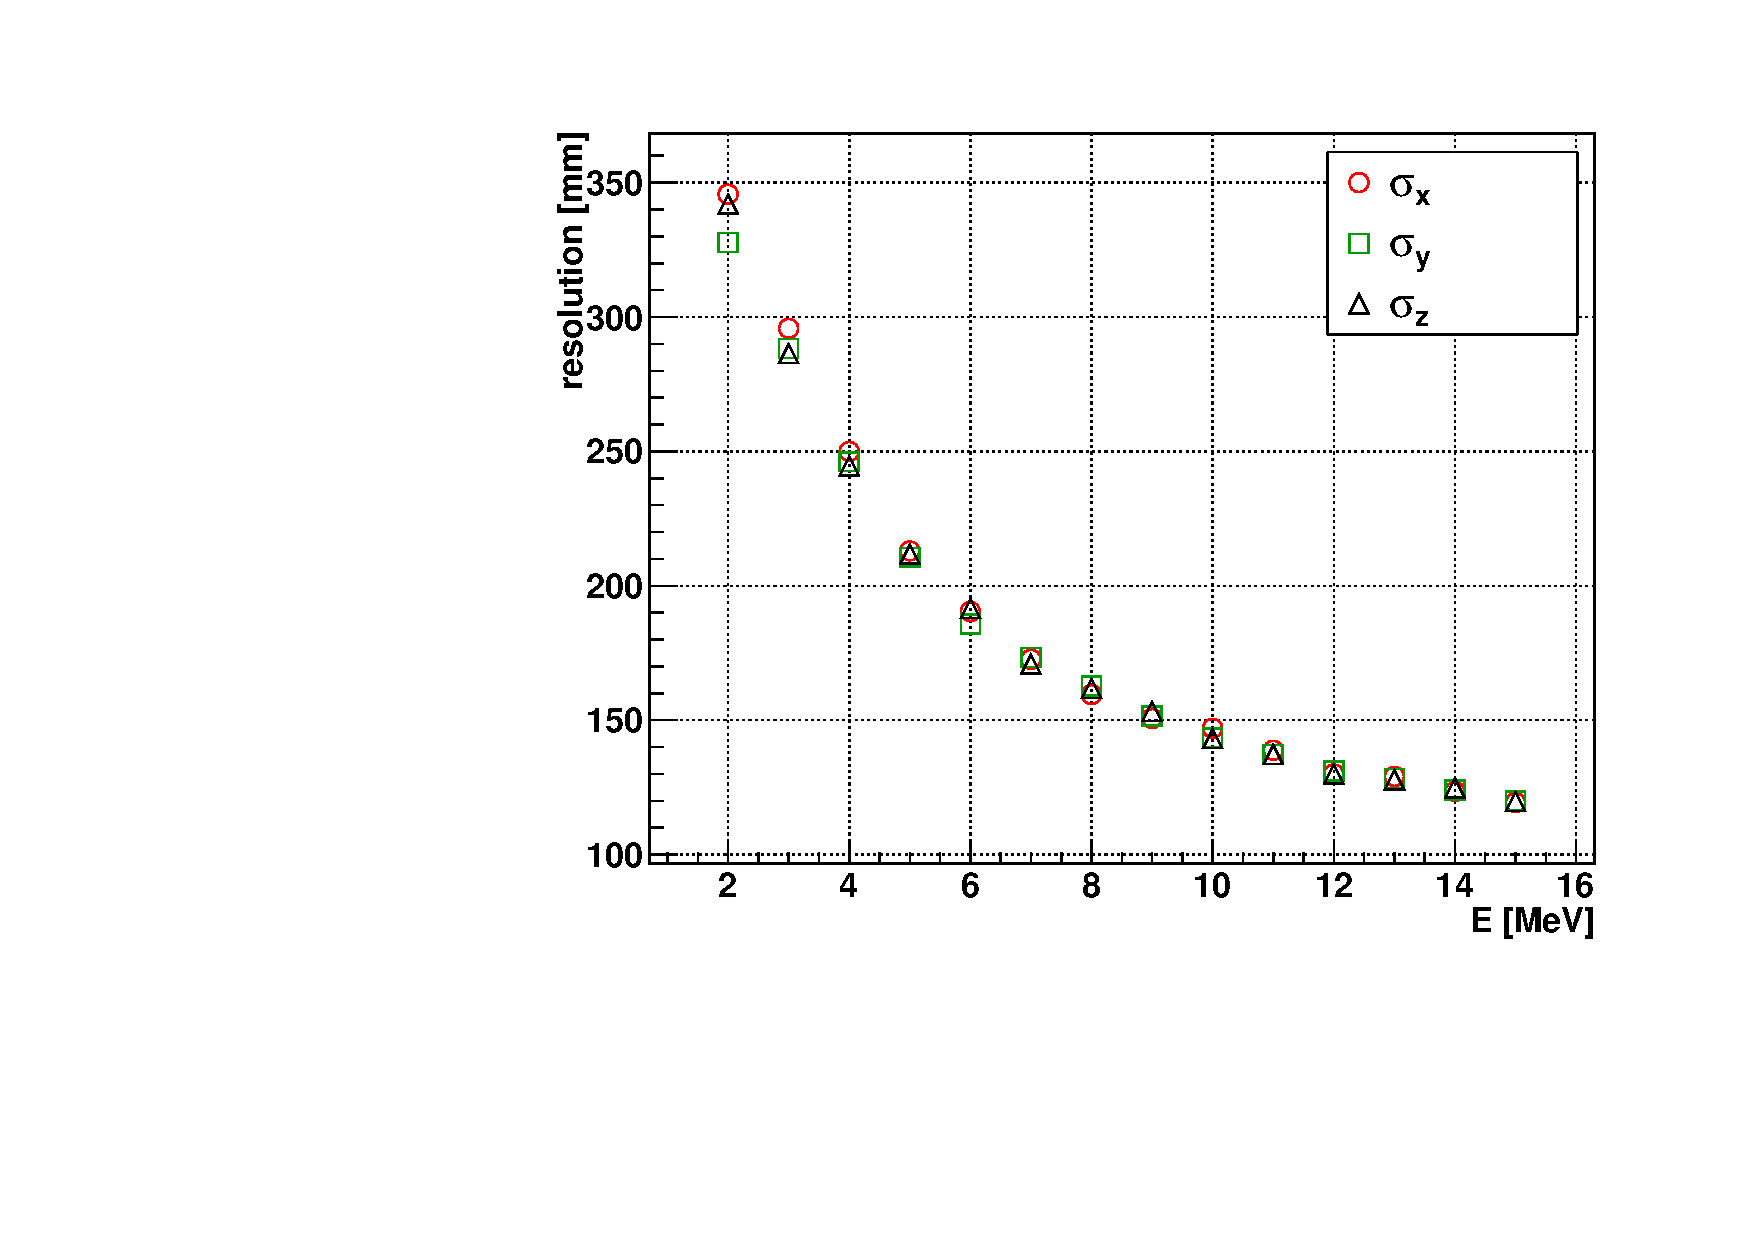
\includegraphics[width=9cm]{MPW_isoFill_posResolVsE.pdf}
	\caption[The \texttt{MPW fitter} fit position resolutions ($\sigma_{x,y,z}$) as a function of energy.]{The \texttt{MPW fitter} fit position resolutions in x (red circle), y (green square), and z (black triangle) axes as a function of energy.}
	\label{fig:MPWposResol_isoFill}
\end{figure}

To check the radial dependence of reconstruction performance, simulations were performed with 5 MeV electrons generated (with an isotropic orientation, and uniformly in azimuth and elevation angles) within each of eleven concentric shells. The centers of these shells were at the AV center, and their inner and outer radii were at $r, r+0.001$ m, where $r$ ranged from 0.5 m to 5.5 m with a step of 0.5 m. Fig.~\ref{fig:FitBiasVsShell} and Fig.~\ref{fig:FitResolVsShell} show the fit position bias and resolution respectively. Evidently fit position bias is rather stable across the differing radii, but resolution deteriorates for events close to the AV wall, or $R>5$ m. This is called the ``near AV effect'', and it was observed in the SNO experiment. For events that occur close to the AV wall, the plexiglass can serve as a lens that distorts the light path \cite{brice1996monte}. A complicated calculation to encompass this complication, and a technique called the ``Near AV cut'', are discussed in Refs.~\cite{coulter2013modelling,jones2011background}, but they are not applied in this thesis. 

\begin{figure}[htbp]
	\centering	
	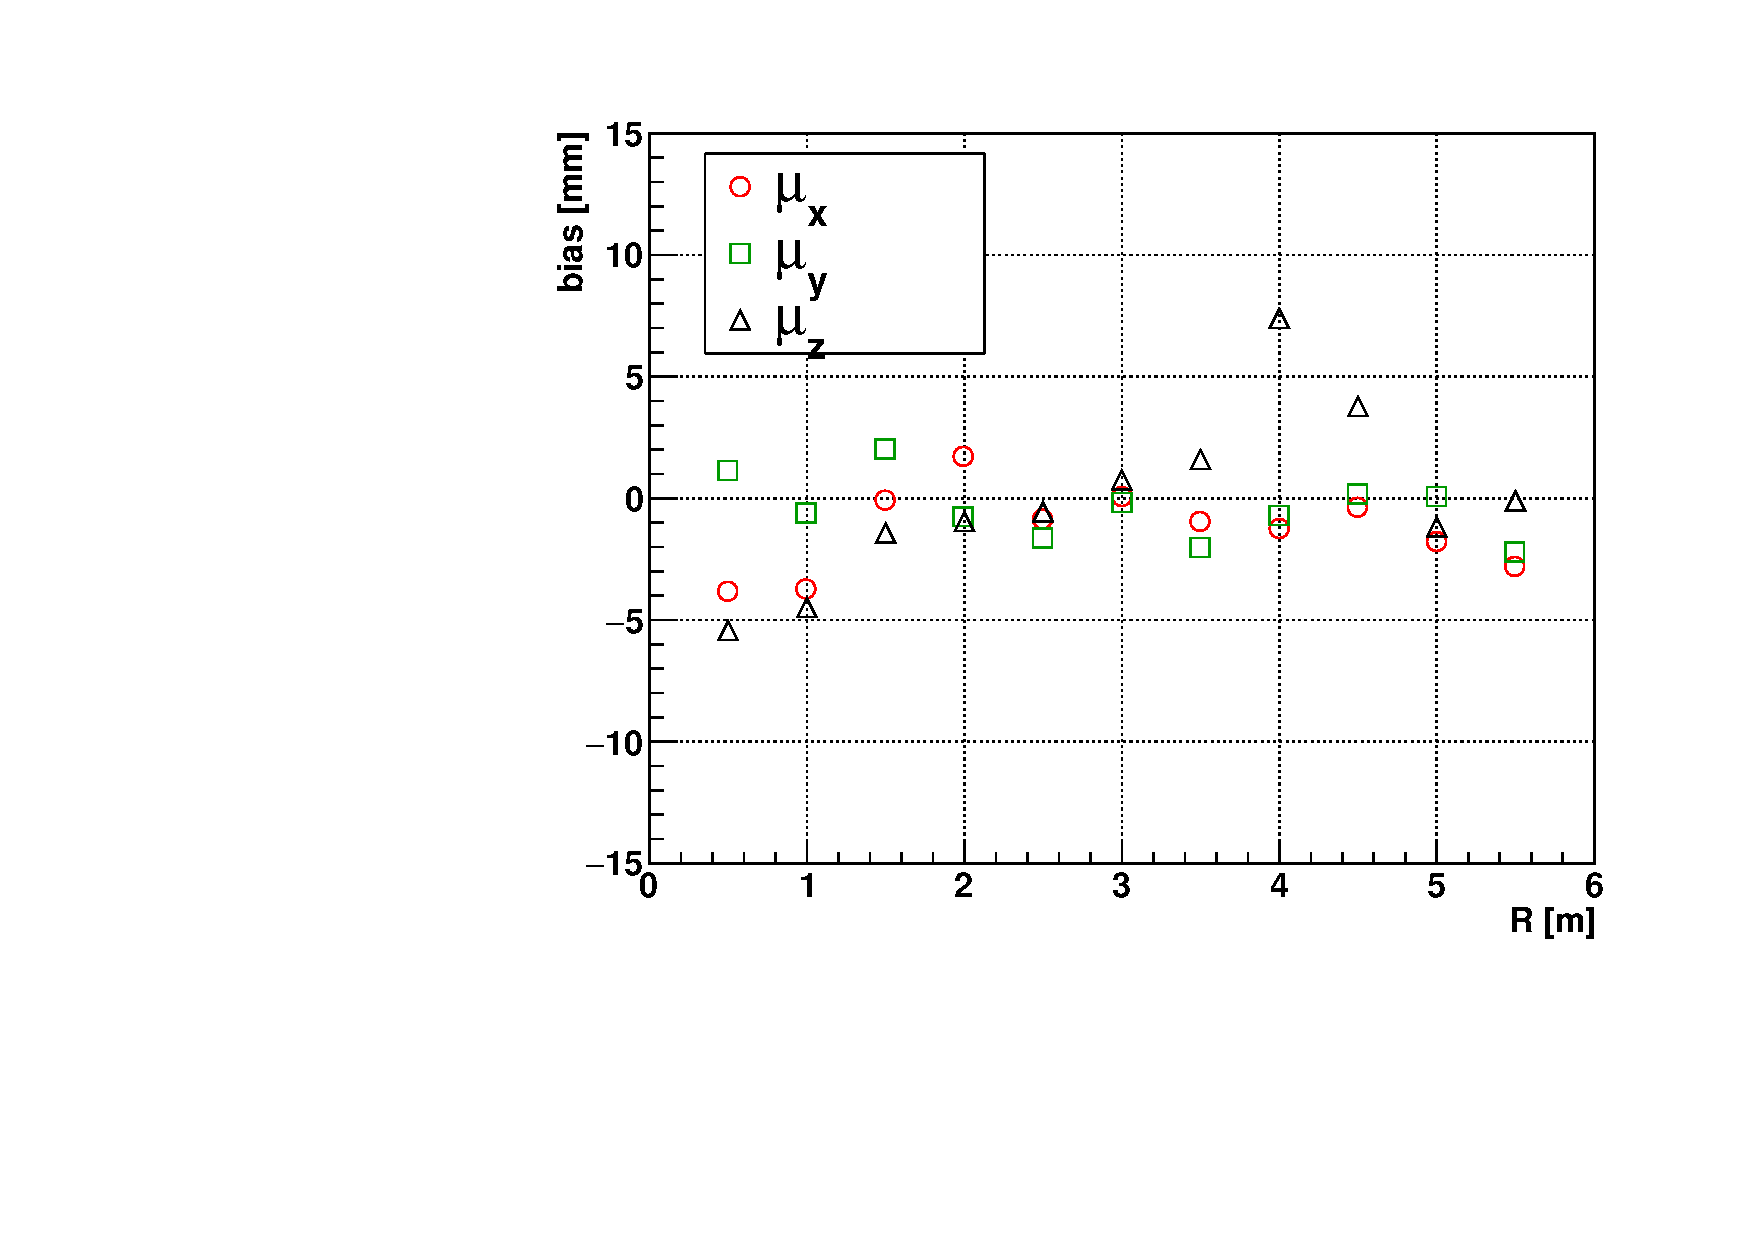
\includegraphics[width=9cm]{shellTest_RvsBias.pdf}
	\caption[The \texttt{MPW fitter} fit position biases ($\mu_{x,y,z}$) as a function of energies.]{The \texttt{MPW fitter} fit position biases of x (red circle), y (green square), and z (black triangle) axes as a function of radius.}
	\label{fig:FitBiasVsShell}
\end{figure}

\begin{figure}[htbp]
	\centering	
	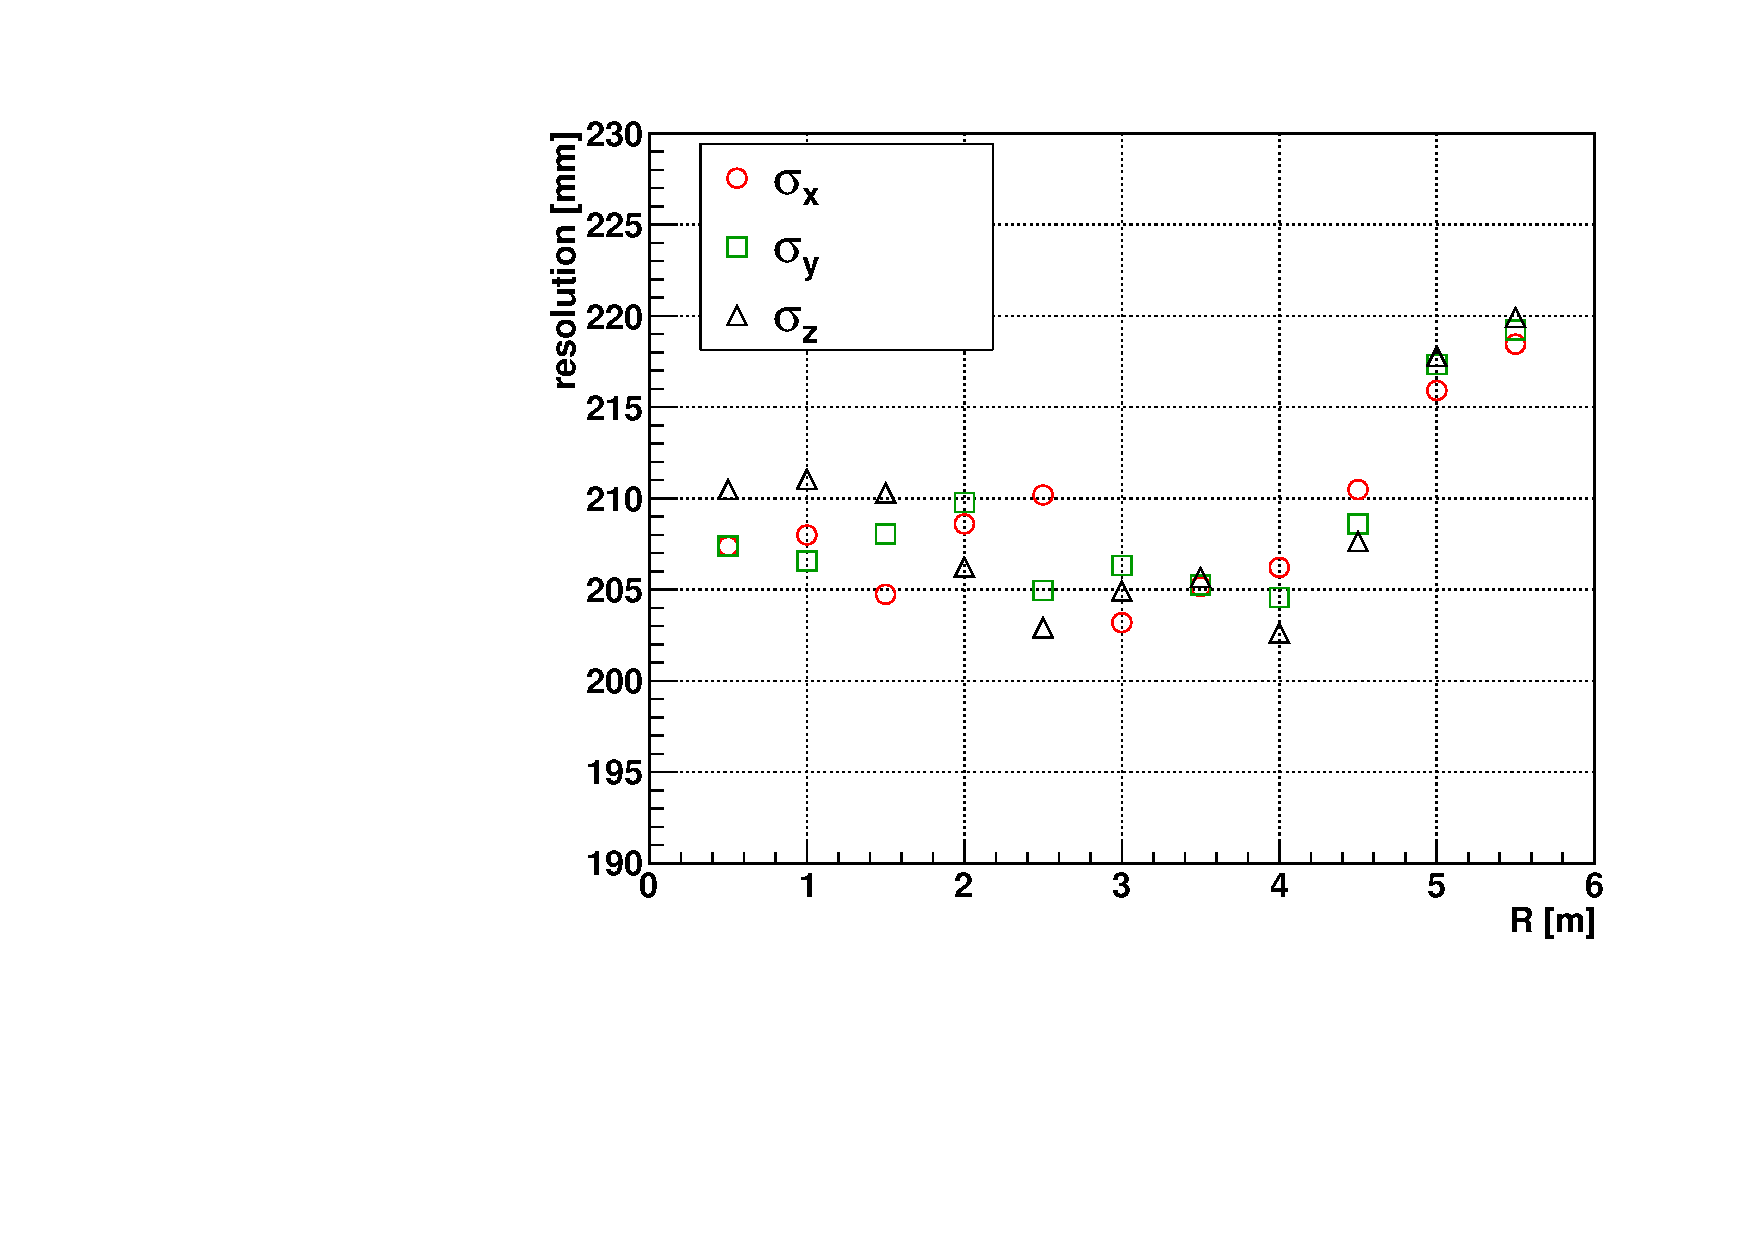
\includegraphics[width=9cm]{shellTest_RvsResol.pdf}
	\caption[The \texttt{MPW fitter} position resolutions ($\sigma_{x,y,z}$) as a function of energies.]{The \texttt{MPW fitter} position resolutions of x (red circle), y (green square), and z (black triangle) axes as a function of radius.}
	\label{fig:FitResolVsShell}
\end{figure}
 
\subsection{Performances of the Direction Reconstruction in water}\label{sect:directResol}

The bias between the true event direction (unit vector $\vec{u}_{\mathrm{MC}}$) and the reconstructed direction (unit vector $\vec{u}_{\mathrm{fit}}$) is described by the angle ``$\theta_e$'', defined as $\cos\theta_e \equiv \vec{u}_{\mathrm{fit}} \cdot \vec{u}_{\mathrm{MC}}$. To describe the distribution of $\cos\theta_e$, an empirical function for the angular resolution was adopted by SNO\cite{boulay2004direct} and it is defined as a combination of two exponential components,
\begin{equation}\label{eq:directResol}
P(\cos\theta_e)=\alpha_M\frac{\beta_M\exp[-\beta_M(1-\cos\theta_e)]}{1-\exp(-2\beta_M)}+(1-\alpha_M)\frac{\beta_s\exp[-\beta_s(1-\cos\theta_e)]}{1-\exp(-2\beta_s)},
\end{equation}
where the parameters $\beta_M$ and $\beta_S$ are the ``decay'' constants or the ``slopes'' of the two exponential components, and $\alpha_M$ adjusts the relative weighting (or blending) of the two exponential components. The first component is due to single scattering of the electrons and represents the true angular resolution of the detector, while the second component, which has a broad tail, is mainly due to the multiple scattering of electrons; this broad tail also includes back-scattering on detector components and poorly reconstructed events \cite{boulay2004direct}. Fig.~\ref{fig:directionResol_5MeV} shows the $\cos\theta_e$ distribution for 5 MeV $e^-$ particles generated at the detector center, with isotropic directions.

\begin{figure}[htbp]
	\centering
	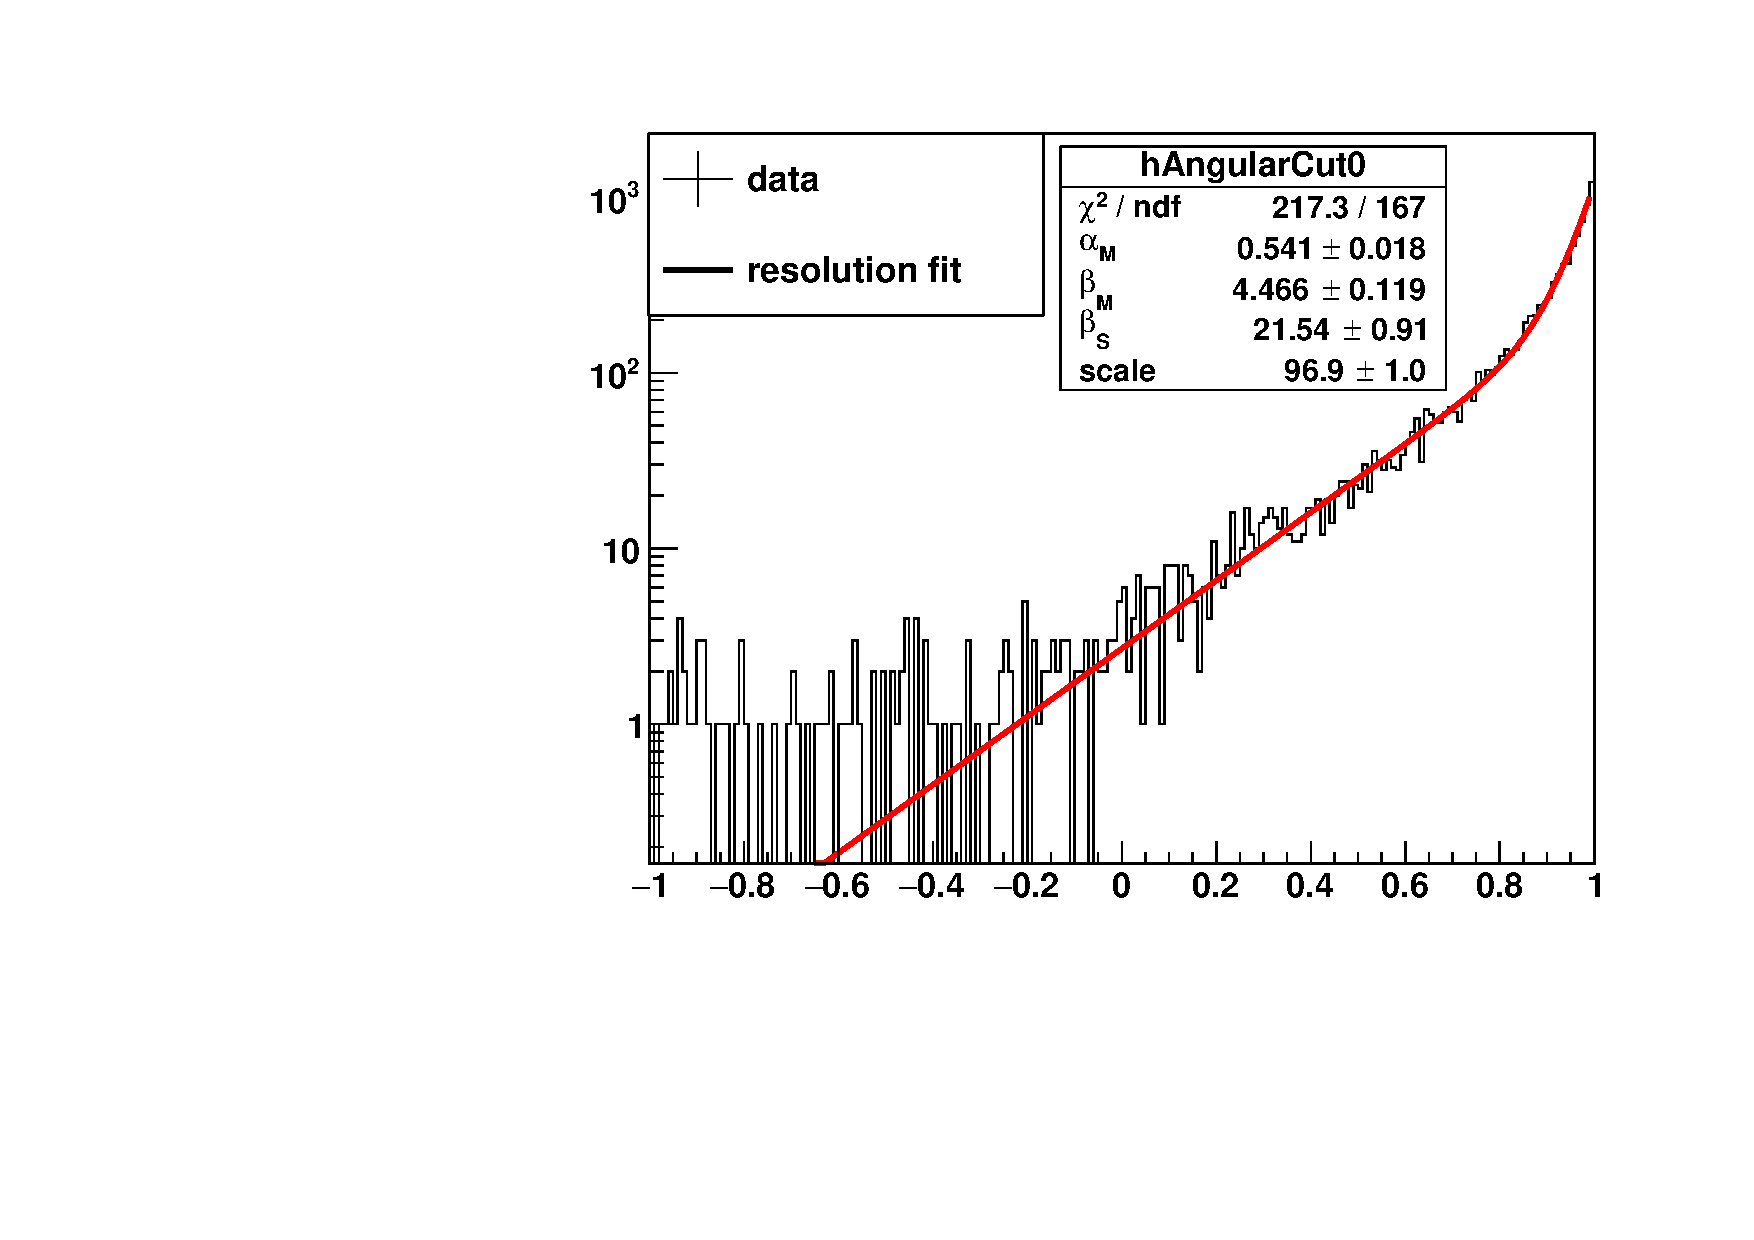
\includegraphics[width=8cm]{MPW_waterDirection_5MeV.pdf}
	\caption[The bias between the fitted and true (MC) direction.]{The bias between fitted and true (MC) direction, fitted with the resolution function $P(\cos\theta_e)$. The MC simulation generated $10^4$ 5 MeV electrons at the detector's center.\label{fig:directionResol_5MeV}}%{John: Axis labels are missing from this figure, and should be added. Also, the legend doesn't match what is plotted!}
\end{figure}

Another way to quantify the performance of the reconstruction is to calculate the angles that contain 50\%, 80\%
or 90\% of the reconstructed events, denoted by $\cos\theta_{0.5}$, $\cos\theta_{0.8}$ and $\cos\theta_{0.9}$ respectively\cite{coulter2013modelling}. Their values (represented in Eqn.~\ref{eq:cosTheta_fraction} by the abstract $\cos\theta_{a}$) are obtained by solving:
\begin{equation}\label{eq:cosTheta_fraction}
\frac{\int_{\cos\theta_{a}}^1 P(\cos\theta_e) \, d\cos\theta_e}{\int_{-1}^1 P(\cos\theta_e) \, d\cos\theta_e} = a\times 100\% \, ,
\end{equation}
where $P(\cos\theta_e)$ is the direction resolution function with the best fit parameters. A larger $\cos\theta_{a}$ means the $\cos\theta_e$ distribution is more peaked around +1, and implies a better direction reconstruction. The results of this analysis for direction resolution, listed in Table.~\ref{tab:angularResol_MPW}, are slightly better than those obtained from the SNO fitter results for the 5-MeV $e^-$ in heavy water, for which \cite{boulay2004direct} $(\beta_M=3.348\pm 0.08119, \, \beta_S=19.3\pm 0.6929)$. Fig.~\ref{fig:diResolVsShell_5MeV} shows the direction resolution parameters $\beta_M$ (left plot) and $\beta_S$ (right plot) as a function of event radial position, based on the simulations described in Sect.~\ref{sect:waterFitterVertex}

\begin{table}[ht]
	\caption{Direction resolutions for the reconstruction of 5 MeV $e^-$ events.\label{tab:angularResol_MPW}}
	\vspace{2mm}
	\centering		
	\begin{tabular*}{110mm}{c@{\extracolsep{\fill}}cccccc}
		\toprule 
	    $\beta_M$ &  $\beta_S$ & $\cos\theta_{0.5}$ & $\cos\theta_{0.8}$& $\cos\theta_{0.9}$\\
        \hline
         4.47$\pm$0.12 & 21.54 $\pm$0.91 & 0.978 & 0.777 & 0.624\\
		\bottomrule	
	\end{tabular*}
\end{table}

\begin{figure}[htbp]
	\centering
	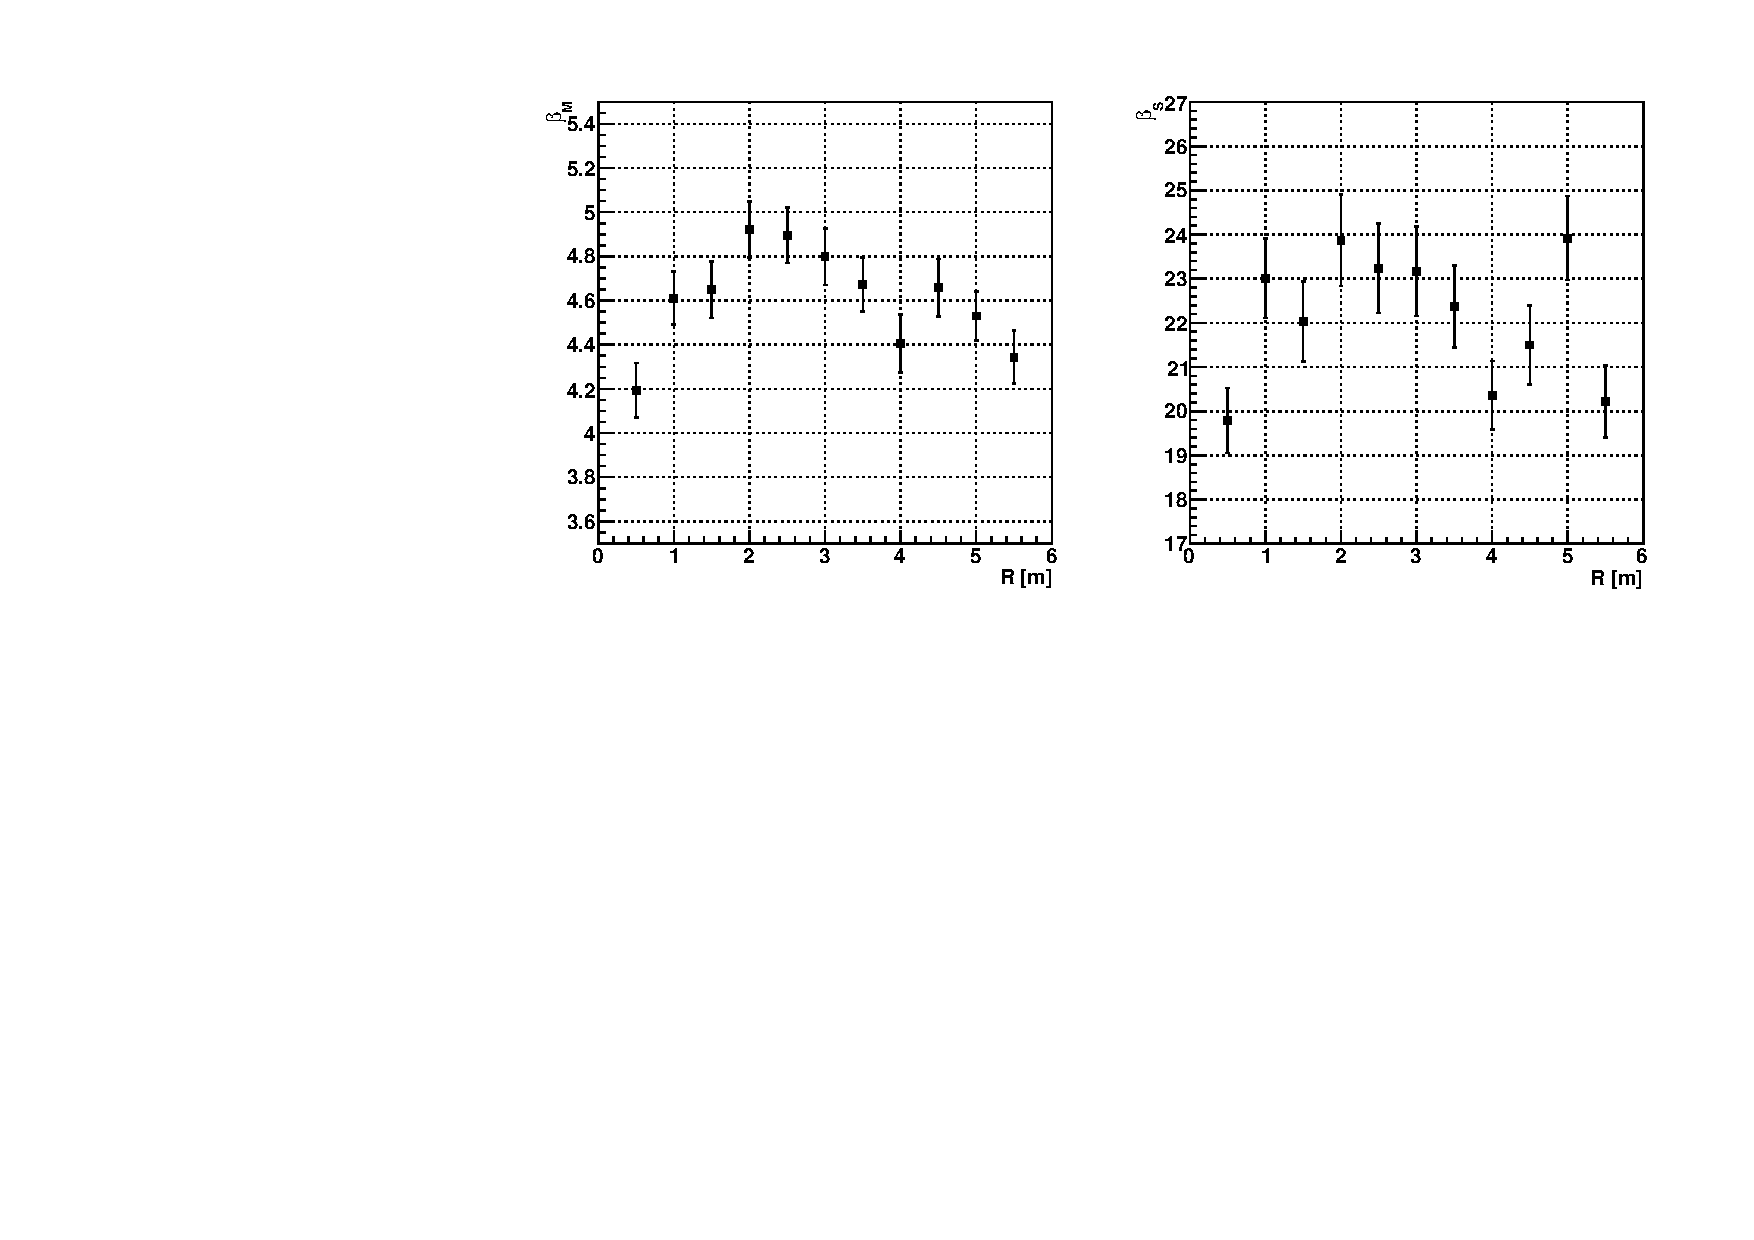
\includegraphics[width=14cm]{DirResolVsShell.pdf}
	\caption[Direction resolutions as a function of radius.]{Direction resolutions as a function of radius. The MC generated 10000 5-MeV $e^-$ inside the AV with isotropic directions.\label{fig:diResolVsShell_5MeV}}
\end{figure}

\subsection{Test on Gamma Events}

For analyzing the AmBe calibration data, reconstructing $\gamma$-events with energies of 2.2 MeV and 4.4 MeV is crucial. When a realistic trigger setting for the antineutrino analysis (taken as that of run-106904) is adopted in simulations, only about 53\% of the (simulated) low energy 2.2-MeV $\gamma$ events triggered a detector response. The event count for simulations was therefore doubled to $2\times10^4$. Table.~\ref{tab:bias_water_gamma} shows the performance (bias and resolution on each axis) of the event position reconstruction for these important gamma events.

\begin{table}[ht]
	\caption{Reconstruction performances for the 2.2-MeV and 4.4-MeV $\gamma$ events.}\label{tab:bias_water_gamma}
	\centering		
	\begin{tabular*}{120mm}{c@{\extracolsep{\fill}}cccc}
		\toprule 
		simulation & $\Delta x \pm \sigma_x$ [mm]& $\Delta y \pm \sigma_y$ [mm]&$\Delta z \pm \sigma_z$ [mm] \\
		\midrule
		2.2-MeV  & $2.278\pm 626.927$ & $-5.663\pm 608.182$& $-10.523\pm 626.034$\\	
		4.4-MeV  & $-6.964\pm364.725$ & $-2.804\pm 368.752$ & $-1.342\pm 368.398$\\
		\bottomrule	
	\end{tabular*}
\end{table}

\subsubsection{Test on $^{16}$N Calibration Source Events}

In a more realistic situation, the data collected from the calibration runs were used to evaluate the fitter performance as well as the reconstruction uncertainties. Chapter 5 will discuss the analyses of the $^{16}$N calibration source in detail. For these analyses, rather than the simple Gaussian function used here, a more specific position resolution function was used. It is construct by the distributions of the initial interaction positions of the particles emit from the source, convolved with a Gaussian resolution function. On the other hand, the same direction resolution function was used in Chapter 5. 

\section{Vertex and Direction Reconstruction for the Water-based Wavelength-shifter}\label{sect:WLSfitter}

A reconstruction algorithm was developed to investigate the proposal, mentioned in Sect.~\ref{sect:wbWLS}, for incorporating in the detector a water-based wavelength-shifter. Fig.~\ref{pmt_wls} shows the position distribution of hit PMTs for MC simulated 5 MeV electrons traveling along the positive $x$ direction in the AV. The left panel shows the case when the detector is filled with pure water while the right panel is for water into which is mixed with the wavelength shifter PPO at a concentration of 0.1 ppm (``wbWLS''). For the same set of electron events, the number of hit PMTs (NHits) in wbWLS is about 2.4 times greater than in pure water. Although in the wbWLS medium extra isotropic light is emitted, the Cherenkov ring can still be clearly distinguished, allowing reconstruction of the directionality of events.

\begin{figure}[htbp]
	\centering
	\begin{minipage}[t]{0.48\textwidth}
		\centering
		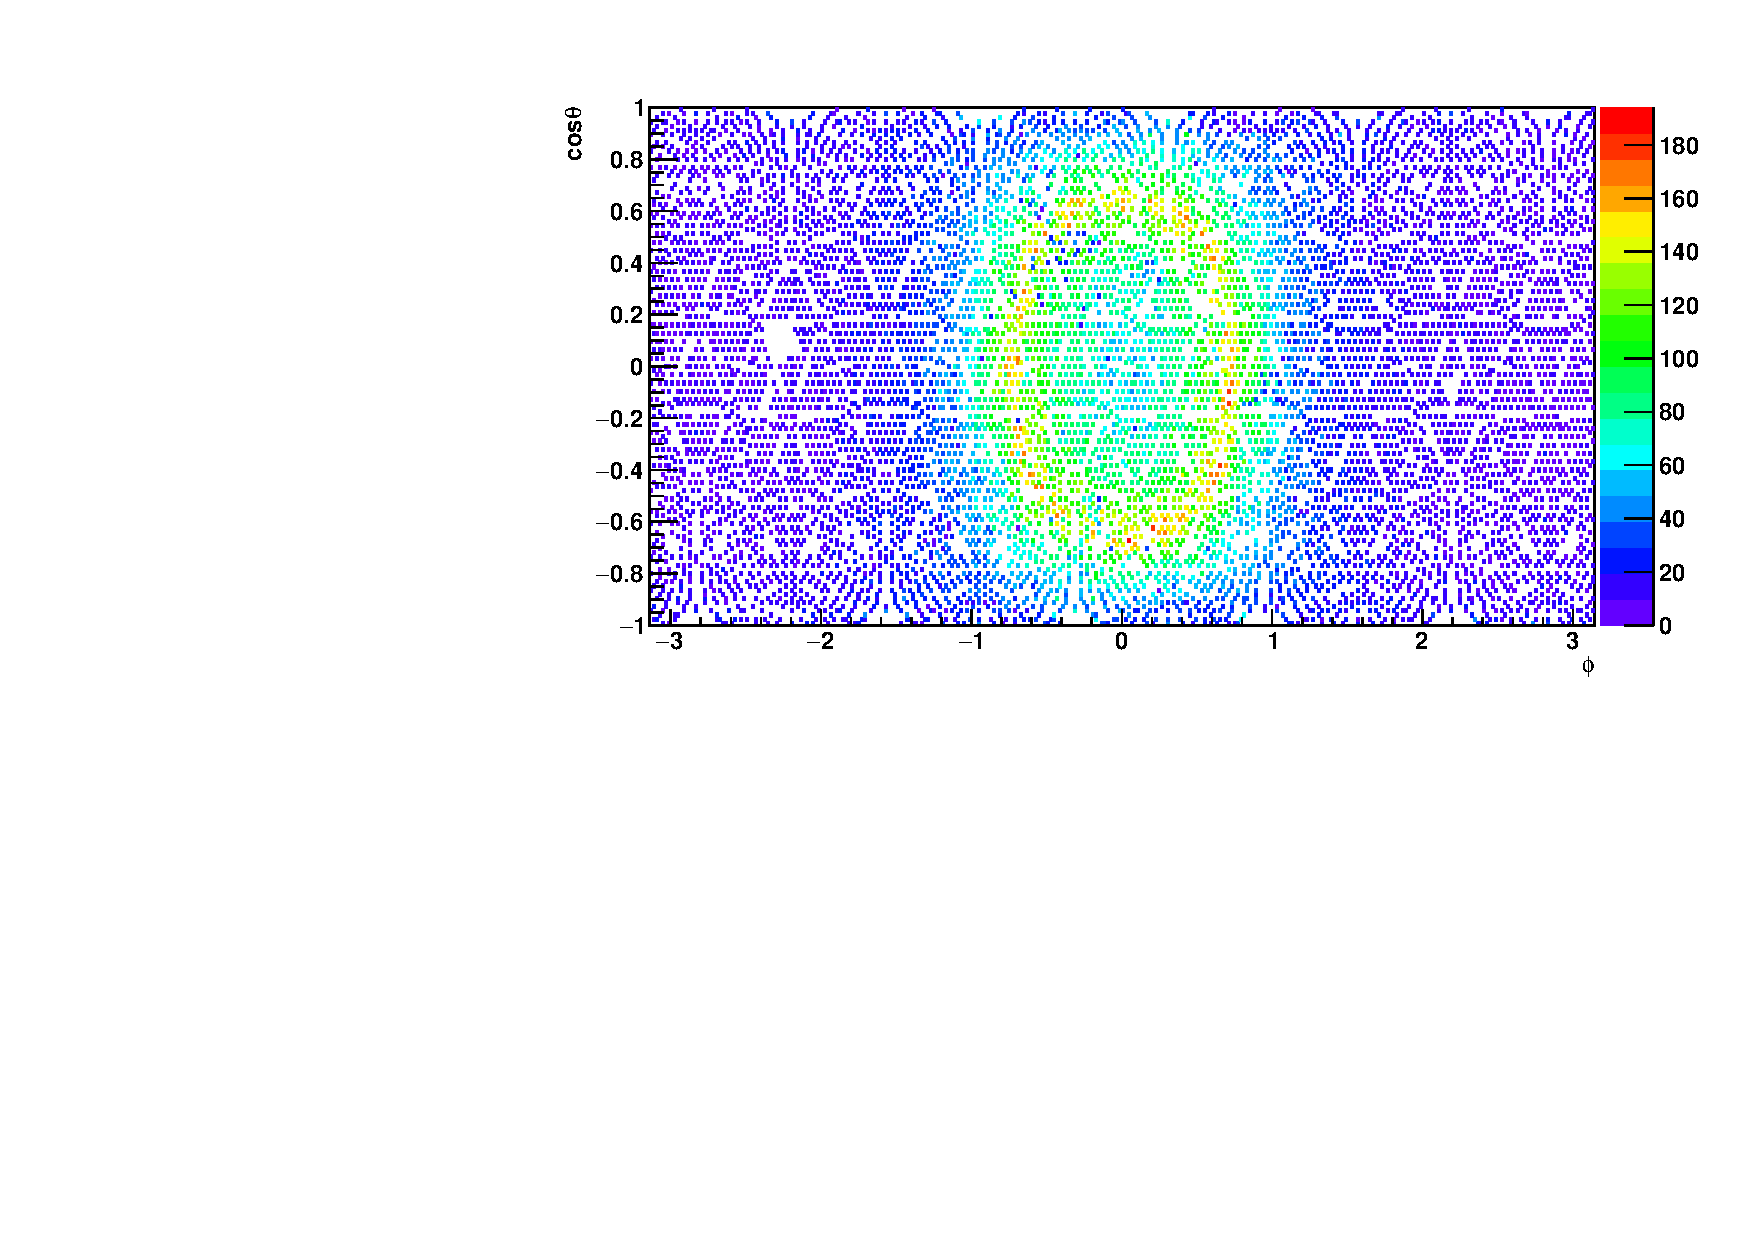
\includegraphics[width=7cm]{PMT_5MeVElectronWater.pdf}
	\end{minipage}
	\begin{minipage}[t]{0.48\textwidth}
		\centering
		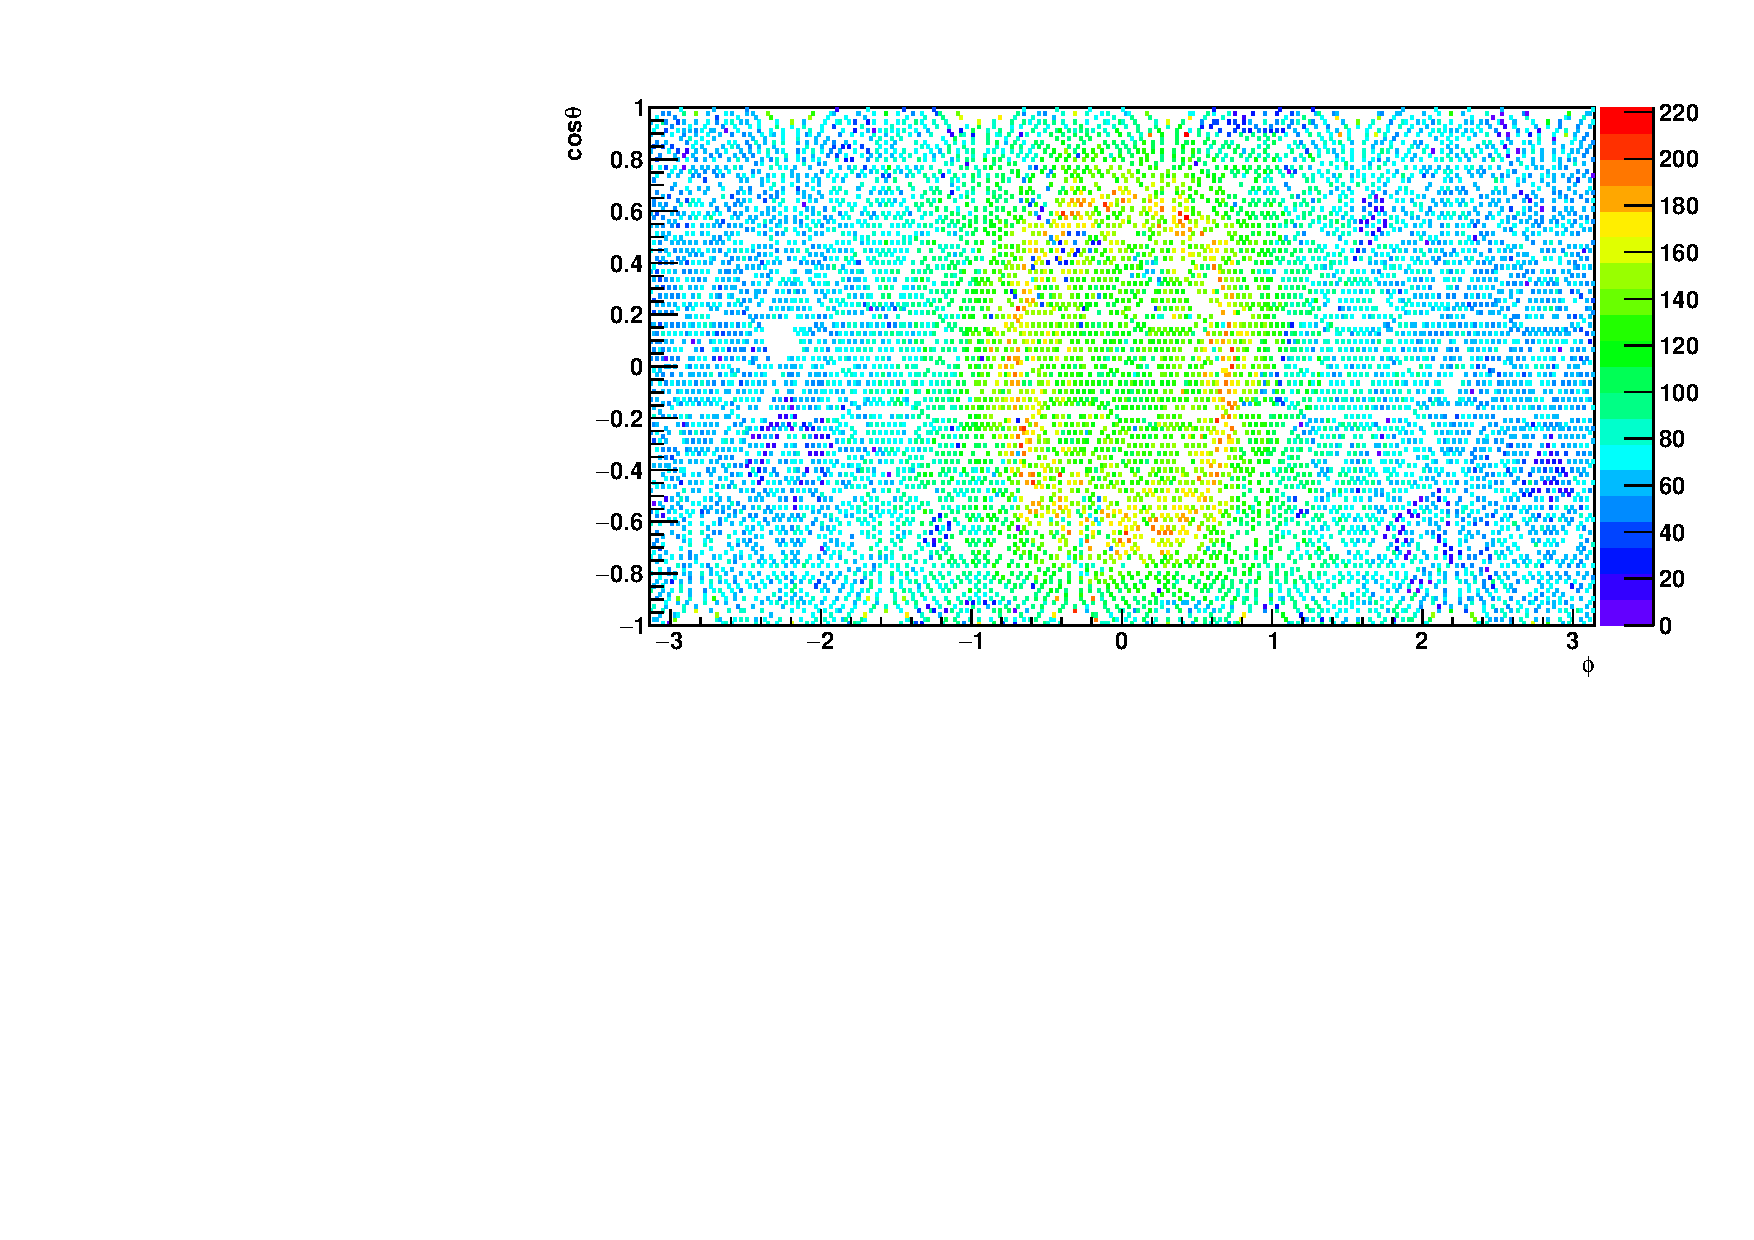
\includegraphics[width=7cm]{PMT_5MeVElectron0p1ppmPPO.pdf}
	\end{minipage}
	\caption[Position distribution of hit PMTs (zenith and azimuth angles).]{Position distribution of hit PMTs (zenith and azimuth angles) for 5 MeV electrons traveling along the $+x$ direction in pure water (left) and water bearing 0.1 ppm PPO (right).\label{pmt_wls}}	
\end{figure}

Fig.~\ref{nhit_wls} shows the energies of simulated electrons as a function of the mean value of the $\mathrm{NHit}$ distribution (mean NHits). In pure water, a 1 MeV electron may cause about 7 PMT hits (but below the detector trigger threshold), while in the wbWLS case the 1 MeV electron simulation results (on average) detecting event with NHits = 20.

\begin{figure}[htbp]
	\centering	
	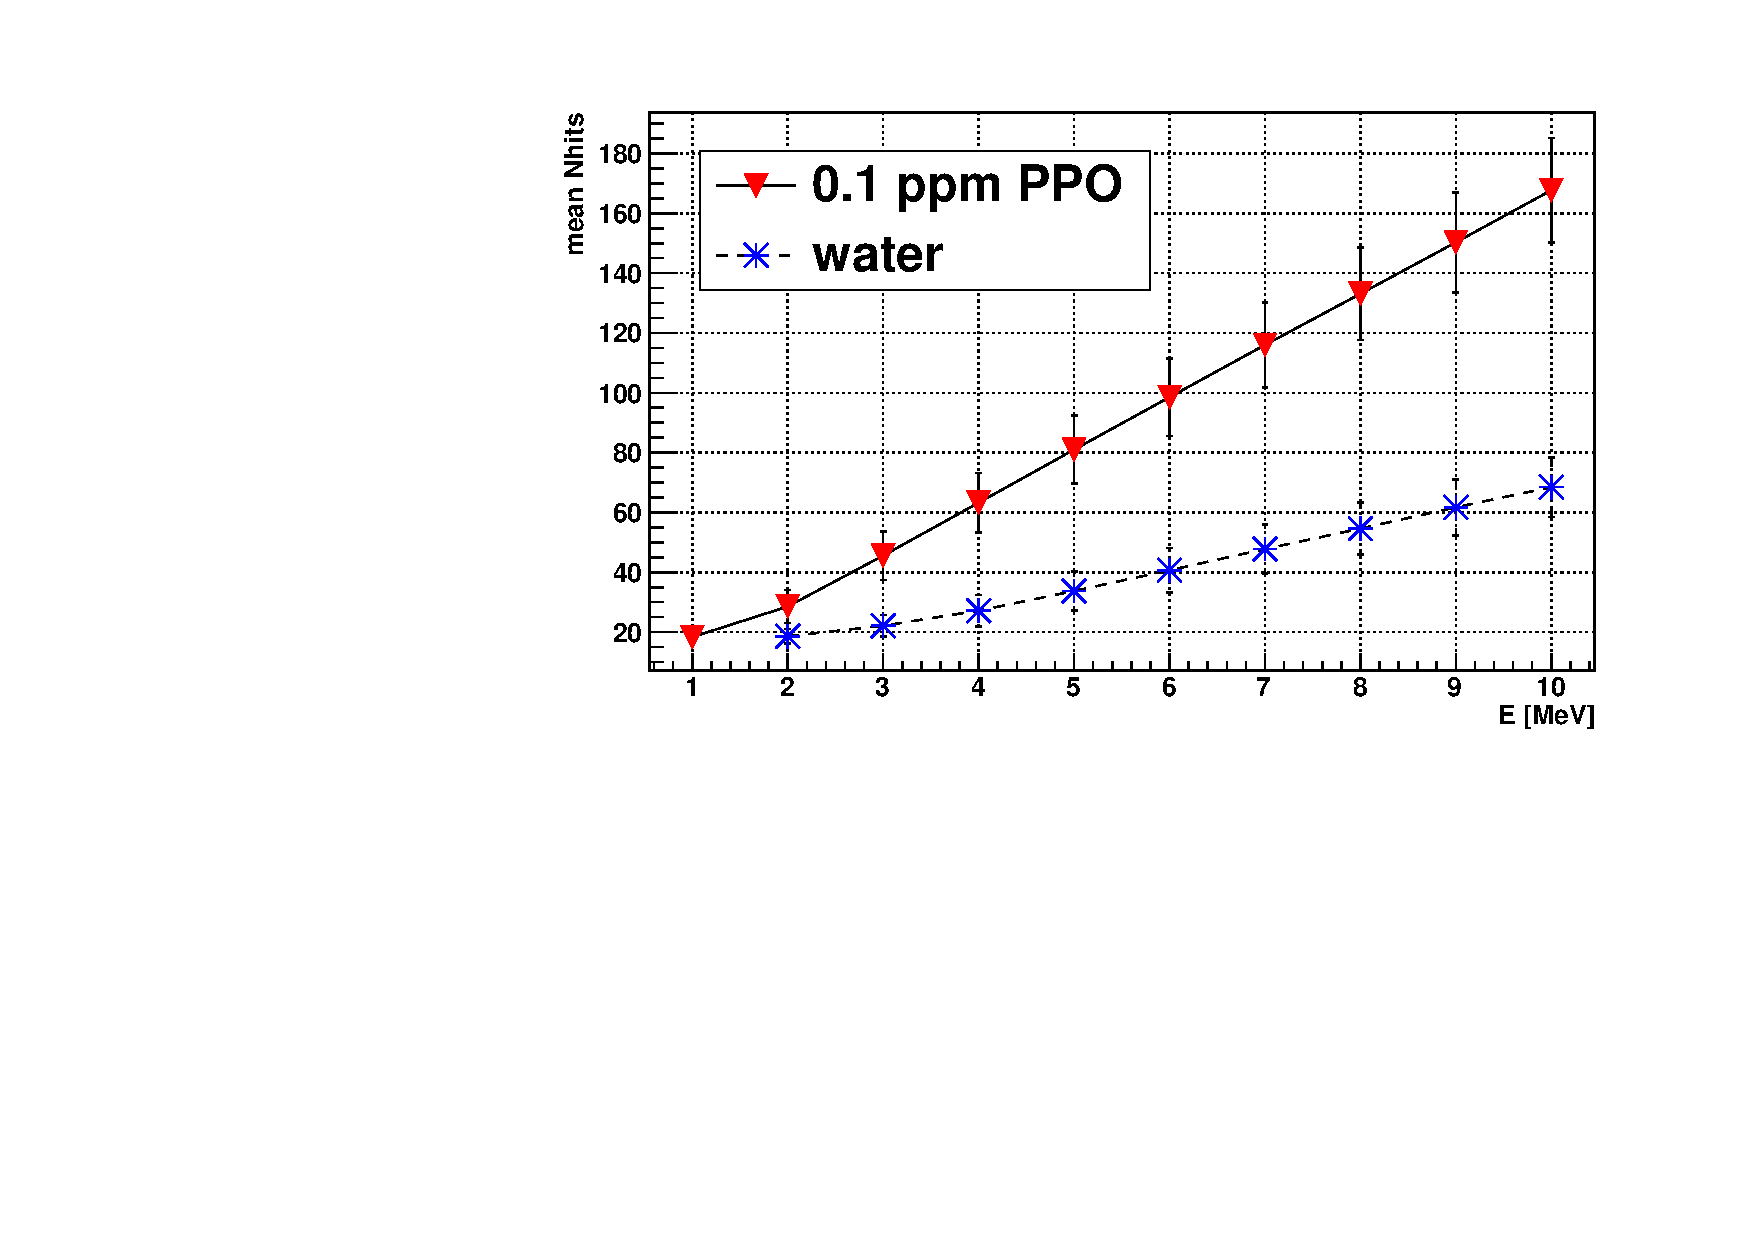
\includegraphics[width=9cm]{nhits_wls.pdf}
	\caption[The energies of simulated electrons as a function of mean NHits.]{The energies of simulated electrons as a function of mean NHits. The values in the 0.1 ppm PPO (solid line with inverted triangle) are compared with the water (dashed line with star).	\label{nhit_wls}}
\end{figure}

In the wbWLS case, since the WLS absorbs and re-emits photons, the reconstruction mentioned in Sect.~\ref{sect:mpw} is slightly modified to build the \texttt{MP WLS fitter}. Given the optical properties of PPO, the prompt light emitted from an event has a probability of $\sim$0.6 to be absorbed by the WLS and then re-emitted at a vertex that is {\em shifted} along the direction of motion ($\hat{n}$) of the event-originating charged particle. Accordingly the fitter returns a shifted vertex, $\vec{X}_\mathrm{0,shifted}=\vec{X}_0+\mathrm{offset}\cdot\hat{n}$. The offset specified in the fitter, obtained from simulations, is 100 mm. Fig.~\ref{WLS_pdf} shows the timing PDF for the wbWLS, which is the PMT response time modified for photon propagation time in the wbWLS.

\begin{figure}[htbp]	
	\centering		
	\begin{minipage}[b]{0.5\textwidth}			
		%\centering			
		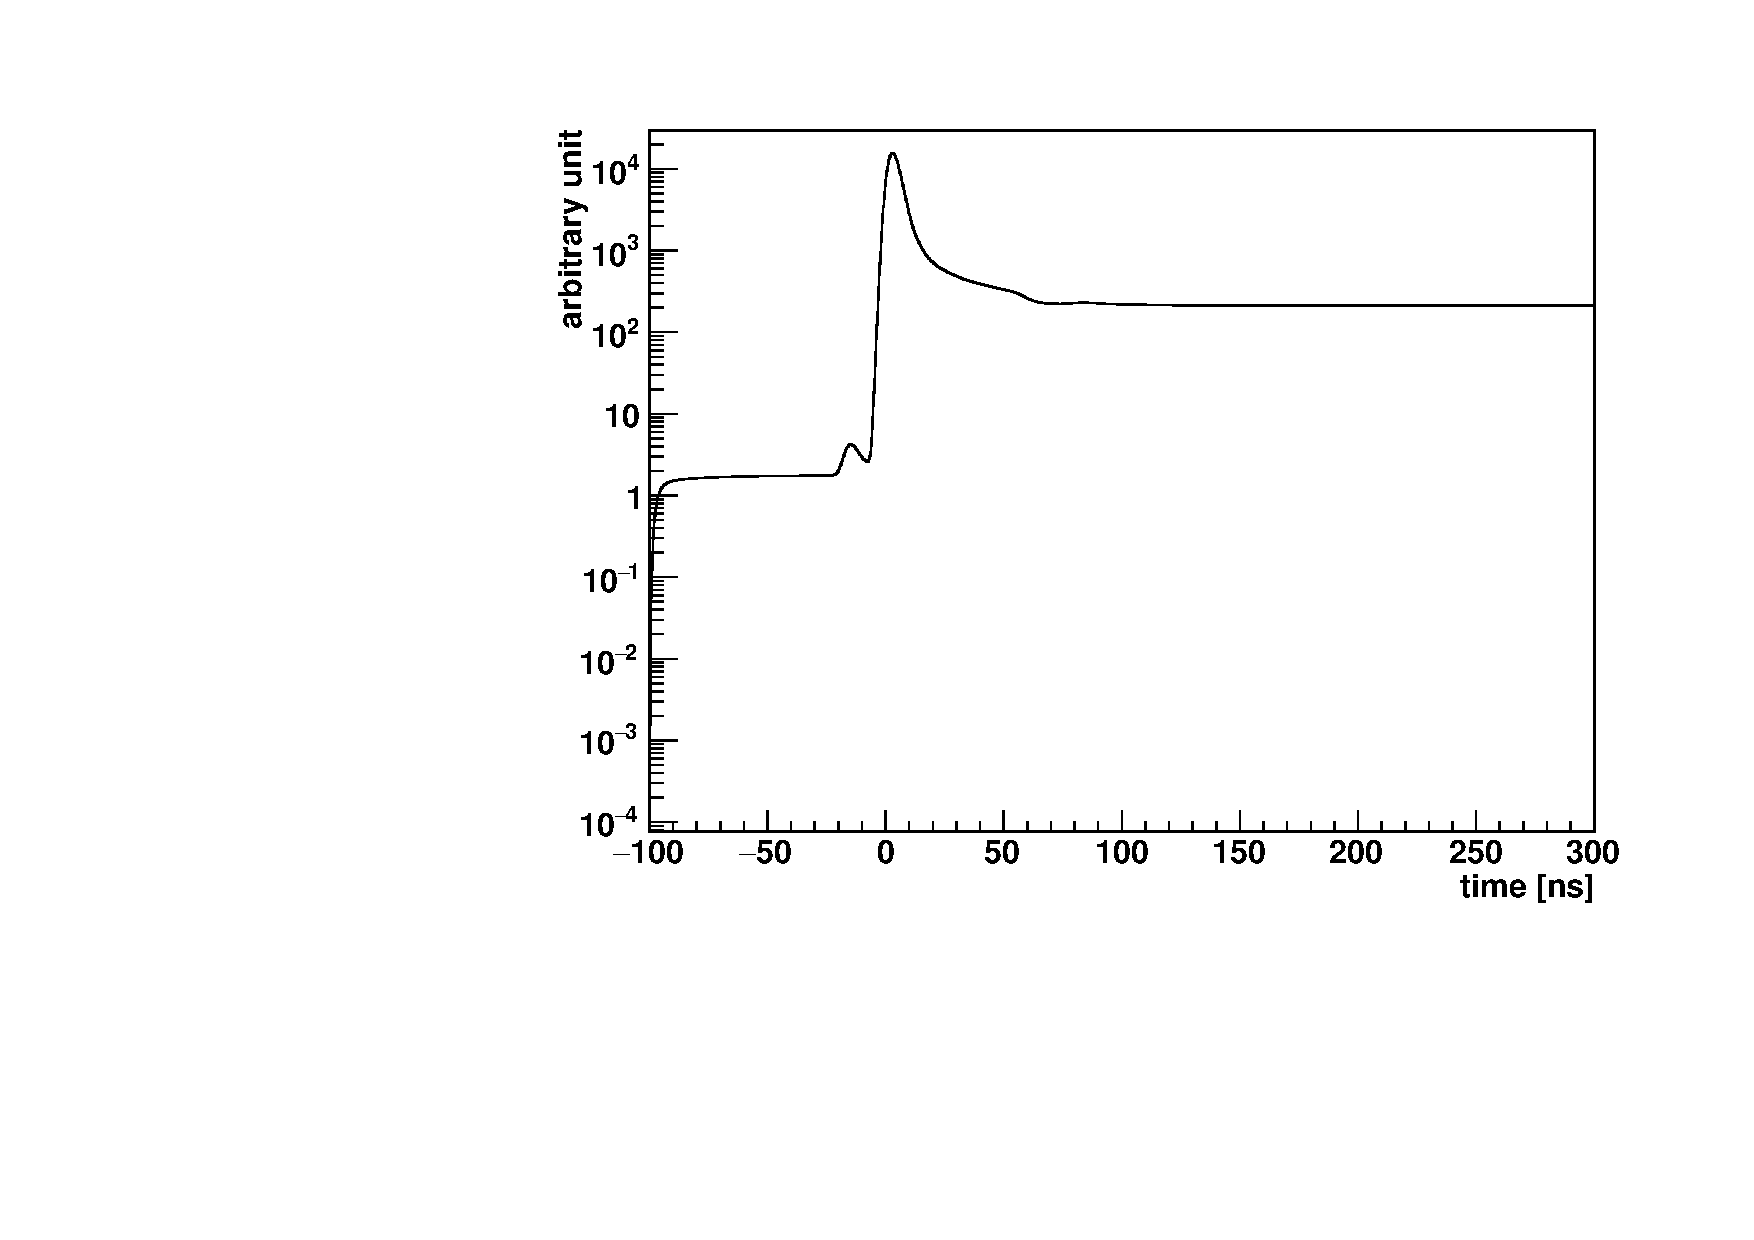
\includegraphics[height=6cm]{WLSTime_pdf.pdf}			
	\end{minipage}%				
%		\begin{minipage}[b]{0.5\textwidth}		
%			%\centering	
%			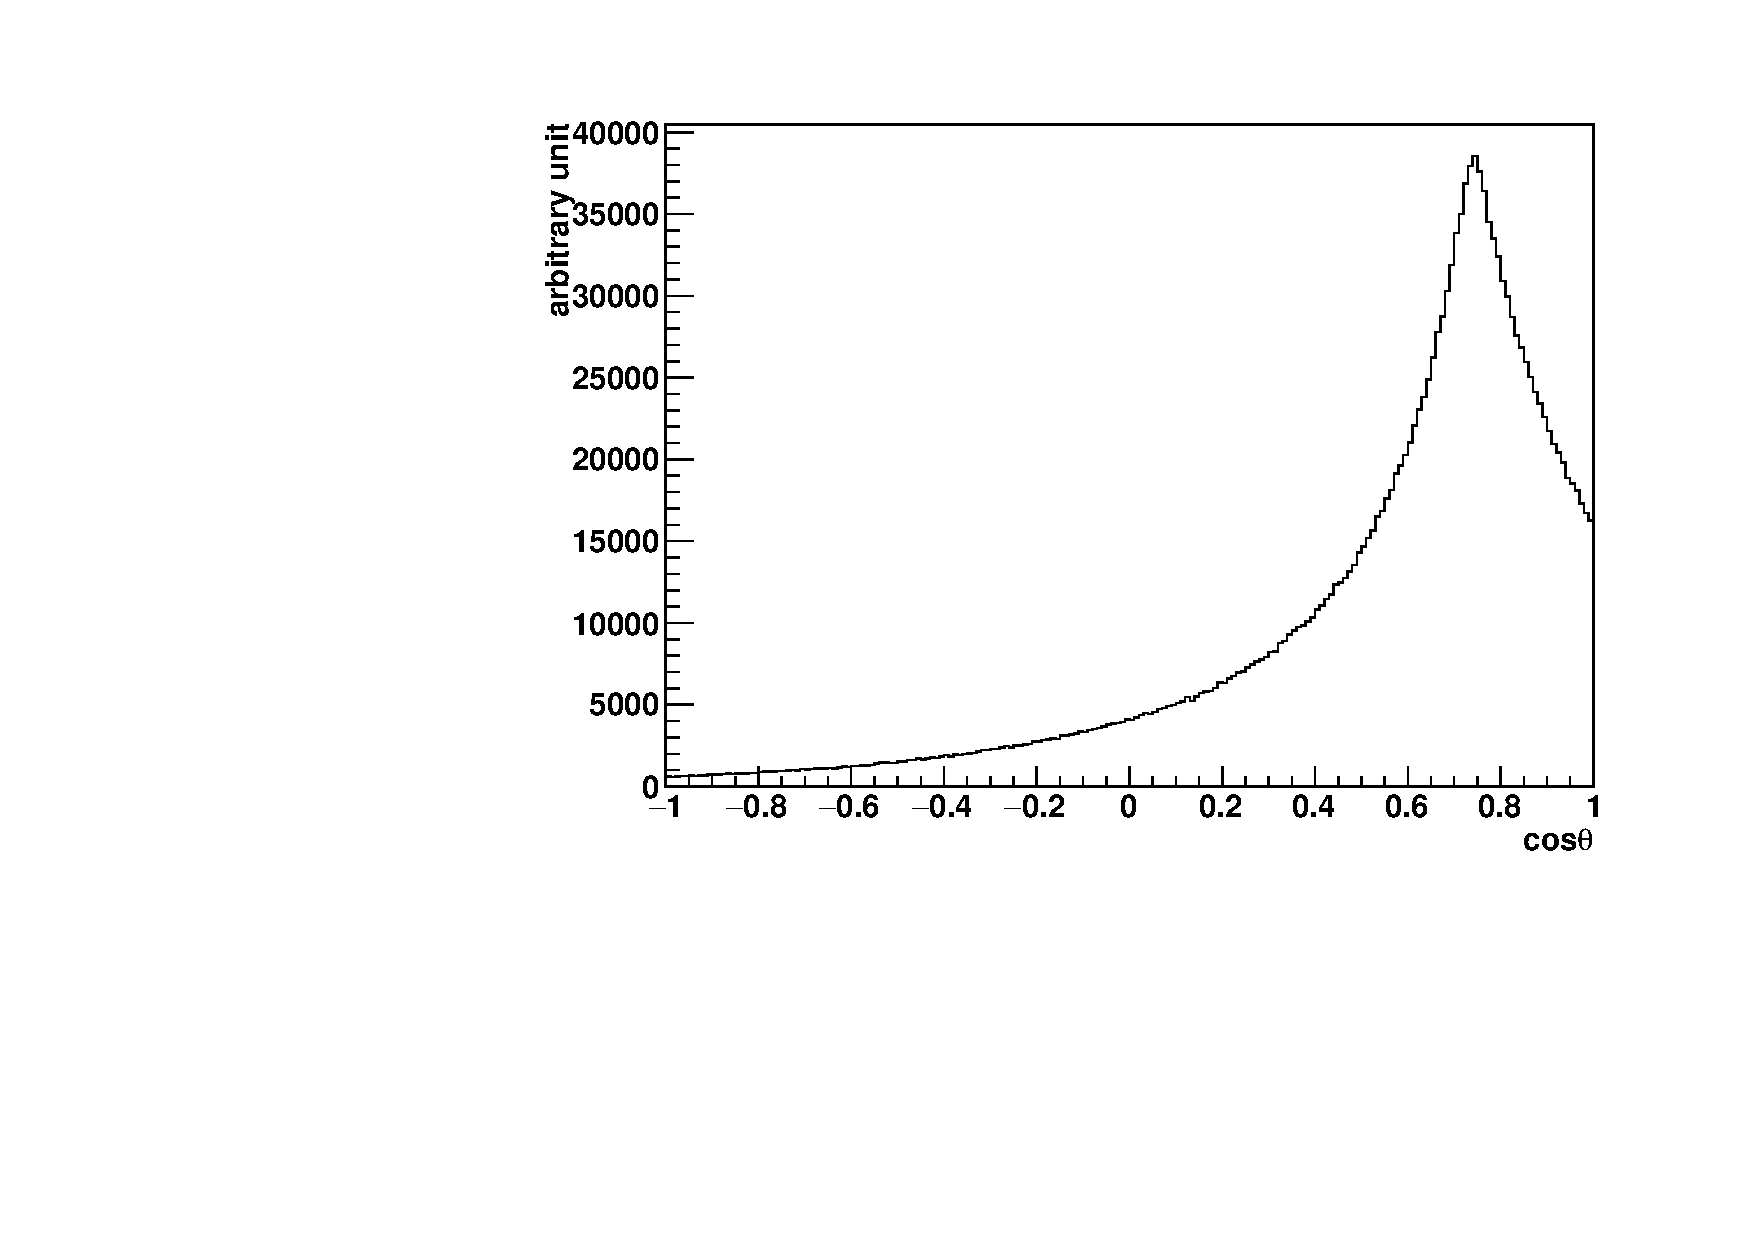
\includegraphics[height=5cm]{ChAngle_pdf.pdf}	
%		\end{minipage}	
	\caption{\label{WLS_pdf} The timing PDF for the wbWLS.}	
\end{figure}

To reconstruct event direction, in addition to the angular distribution of Cherenkov photons, $\cos\theta_{Ch}$, we also consider the fraction of the re-emitted and wavelength-shifted photons that cause a flat (i.e. uniform) angular distribution.

To test the performance of the \texttt{MP WLS fitter}, a simulation was performed with 5 MeV electrons released at the center of the wbWLS-filled AV and traveling along +x direction; and for comparison, the equivalent simulation was also done for the pure water-filled AV, in which case the simulated events were reconstructed by the water fitter. Fig.~\ref{WLSFitPos} shows the performance of the WLS fitter reconstructed positions of the MC simulations, in comparison with the pure water case. For the fit position distribution of 5 MeV $e^-$ in the wbWLS medium, we obtained a root mean square (RMS) position error (i.e position resolution) of 201 mm, and a bias towards the AV center (the mean of histogram) of 29 mm. Compared to the pure water case, the RMS is a 188 mm improvement, and the fit bias is about 19 mm better.

\begin{figure}[htbp]	
	\centering	 		
	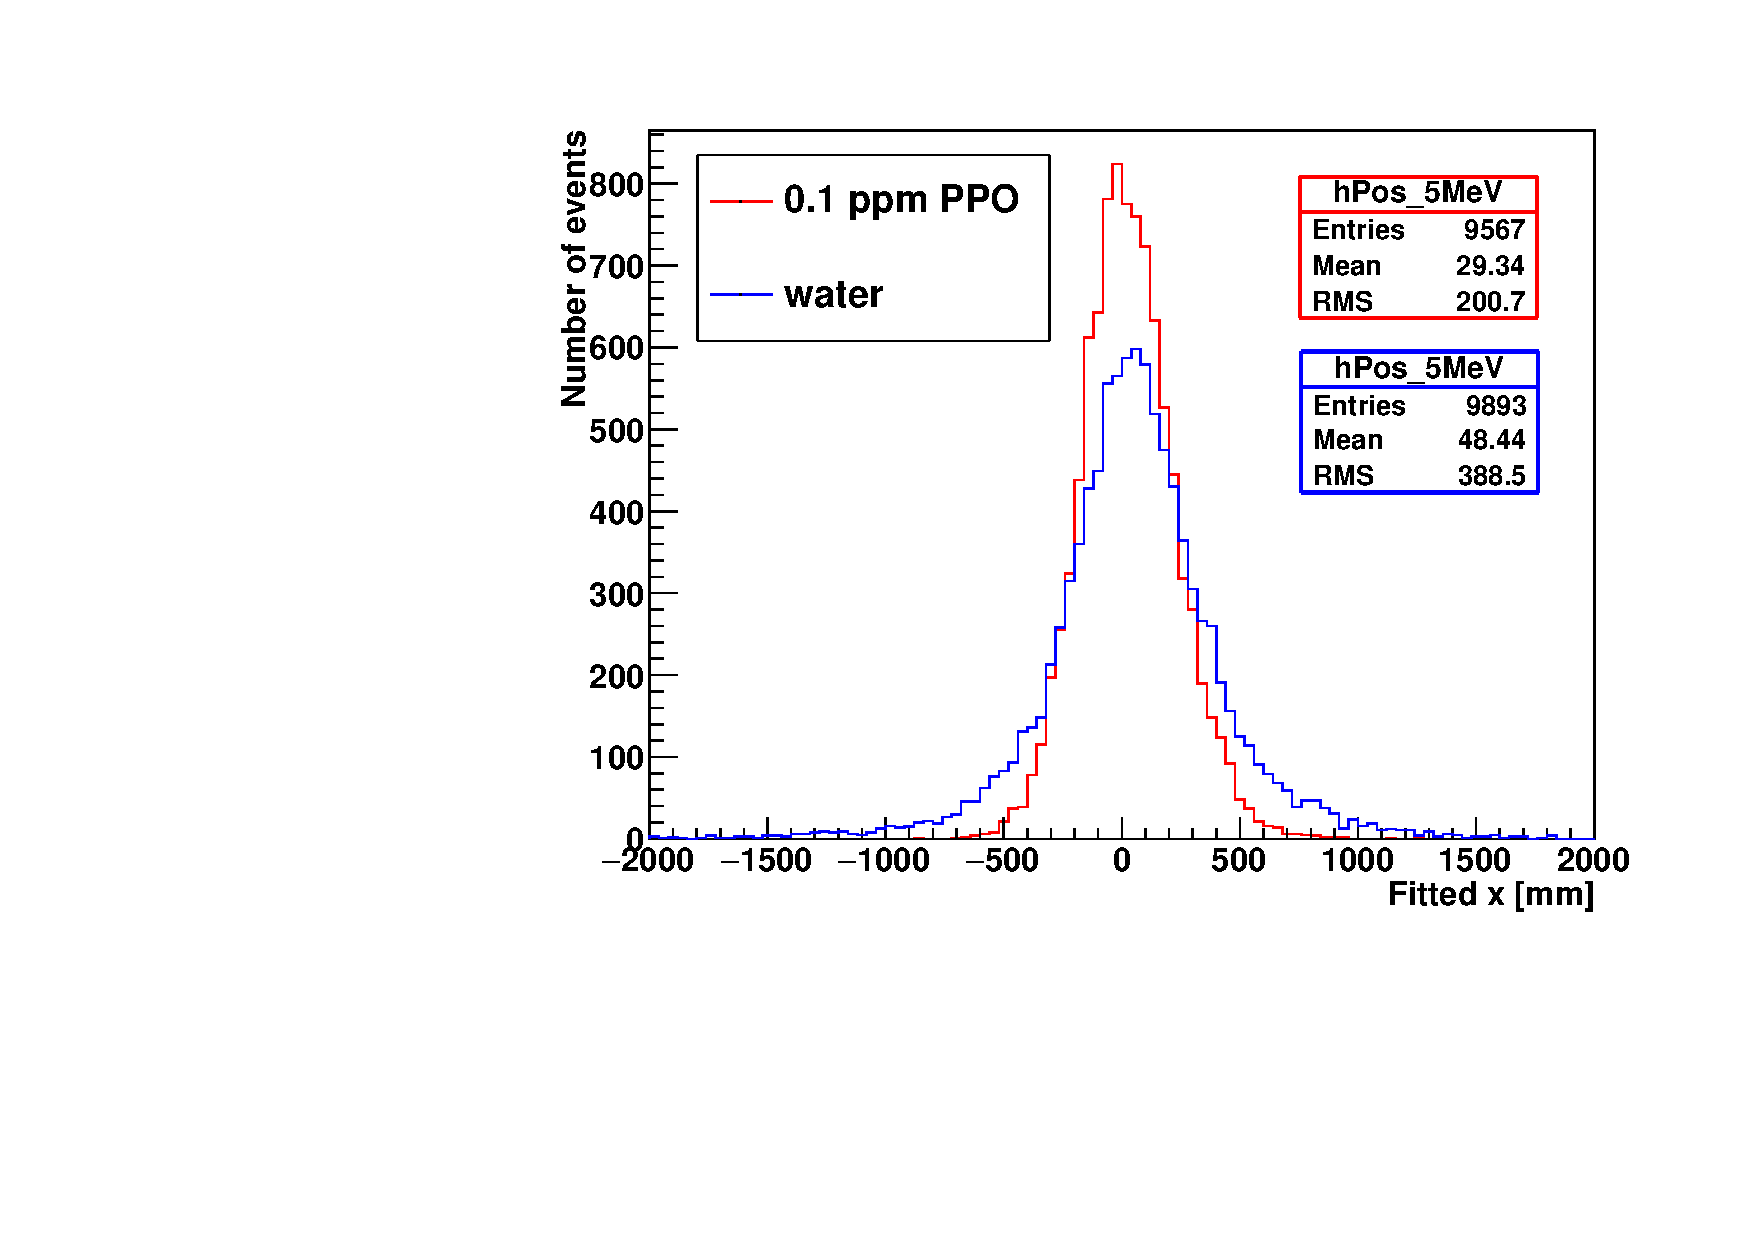
\includegraphics[height=5cm]{WLS_FittedPos.pdf}		
	\caption[Fitted $x$ position.]{Fitted $x$ position. The \texttt{MP WLS fitter} reconstructed $x$ positions of the 5-MeV $e^-$ events in the wbWLS (red) are compared to those in the pure water (blue).\label{WLSFitPos}
	}
\end{figure}

As it had been in Sect.~\ref{sect:directResol}, again here $\cos\theta_a$ in Eqn.~\ref{eq:cosTheta_fraction} was used to characterize the performance of the direction reconstruction. Table.~\ref{tab:quantAngular} compares the \texttt{MP WLS Fitter}'s $\cos\theta_{a}$ values when applied to SNO heavy water data\cite{boulay2004direct}, and to simulations for both SNO+ pure water and SNO+ wbWLS. The best direction reconstruction is obtained for the SNO+ pure water case, with results for the wbWLS case proving less satisfactory (e.g. by about 30\% for $\cos\theta_{0.9}$).
\begin{table}[ht]
	\caption{A comparison of quantitative estimates for the angular resolution for the SNO heavy water, SNO+ wbWLS and the SNO+ pure water cases.\label{tab:quantAngular}}
				\centering		
		\begin{tabular*}{120mm}{c@{\extracolsep{\fill}}cccc}
			\toprule 
			medium & $\cos\theta_{0.9}$ & $\cos\theta_{0.8}$ & $\cos\theta_{0.5}$
			\\
			\midrule
			SNO heavy water  & 0.50 & 0.71 & 0.92  \\	
			SNO+ water  & 0.62 & 0.78 & 0.98	\\
			wbWLS  & 0.37 & 0.63 & 0.90  \\	
			\bottomrule	
		\end{tabular*}
\end{table}

Comparing a pure water SNO+ detector and the wbWLS one, using the \texttt{MP WLS fitter} for physics events gives a better position resolution without significant loss in performance of the direction reconstruction. This \texttt{MP WLS fitter} was also applied in a study of the potential for measuring reactor antineutrinos in the wbWLS-filled SNO+ detector, see Ref.~\cite{mekarski2018electron} for details.

\section{Vertex Reconstruction for the Partial-fill}\label{sect:partialFitter}

The following two sections discuss the vertex reconstruction in liquid scintillator. The vertex reconstructions for the partial-fill and scintillator phases are very similar. Both must accommodate two detection media, water and scintillator, and calculate the light paths in these two regions. I will first describe the calculations in the partial-fill case, since its geometry is more complex, relative to which the full scintillator case can be considered a simplification.

\subsection{Partial-fill}

In the partial-fill geometry, the SNO+ detector can be described as being composed of three parts: the neck cylinder filled with scintillator; the AV sphere, which contains scintillator above and water below the water-scintillator interface (plane); and the water-filled PSUP sphere lying outside the neck and the AV.

If we neglect complications related to the acrylic and other solid parts of the detector, then photons travel in only two media: water and scintillator (see Fig.~\ref{fig:scintpath}). By definition the length of the straight light path from a vertex to a hit PMT position is $|\vec{l}_p|=|\vec{X}_\mathrm{PMT}-\vec{X}_0|$. The \texttt{MP scint-water fitter} evaluates the portion $d_{sp}$ of the total path travelled in scintillator, and length of the path travelled in water obviously is $|\vec{l}_p|-d_{sp}$. Since photons travel at different speeds ($v_\mathrm{gr,scint}$, $v_\mathrm{gr,water}$) in these two media, the \texttt{MP scint-water fitter} evaluates the time of flight, as:
\begin{equation}
t_{\mathrm{transit}} = \frac{|\vec{l}_p|-d_{sp}}{v_\mathrm{gr,water}} +\frac{d_{sp}}{v_\mathrm{gr,scint}} \; .
\end{equation}
Once having computed $t_{\mathrm{transit}}$ the time residual $t_\mathrm{res}$ can be calculated, and the balance of the fitting procedure is the same as in the \texttt{MP water fitter}.

\begin{figure}[!htb]
	\centering
	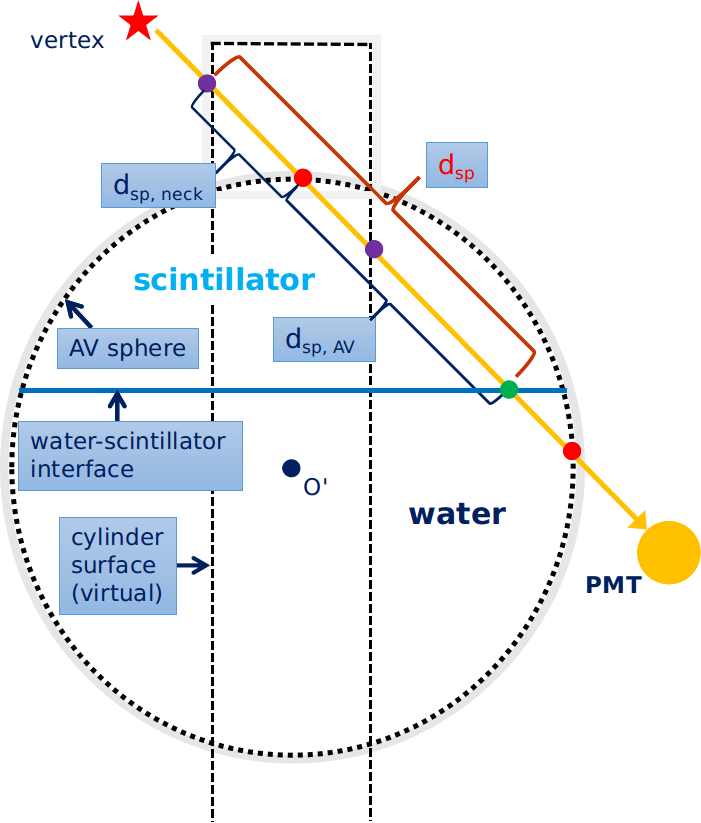
\includegraphics[width=7cm]{scintpath.png}
	\caption[Light path calculation for the \texttt{MP scint-water fitter fitter}.]{Light path calculation for the \texttt{MP scint-water fitter fitter}. In the figure, a light path intersects with the neck cylinder surface, the AV sphere as well as the water-scintillator interface. The total length of the path in the scintillator region (scintillator path, $d_{sp}$) includes the paths in the neck ($d_{sp,\mathrm{neck}}$) and in the AV ($d_{sp,\mathrm{AV}}$). Calculations of the ray-cylinder, ray-plane and ray-sphere intersections are applied.	\label{fig:scintpath}}
\end{figure}

It follows that the crucial part of the calculation is obtaining $d_{sp}$. The light path vector $\vec{l}_p$, encoding length and direction, may intersect and one or more of three geometrical objects: the neck cylinder, the AV sphere, and the water-scintillator interface plane. As illustrated in Fig.~\ref{fig:scintpath}, a detailed calculation of $d_{sp}$ includes evaluation of (1) $\vec{l}_p$ and neck (ray-cylinder) intersection; (2) $\vec{l}_p$ and the AV (ray-sphere) intersection and (3) $\vec{l}_p$ and the water-scintillator interface (ray-plane) intersection. The distance $d_{sp}$ is further separated into path segments within the neck ($d_{sp,\mathrm{neck}}$) and within the AV ($d_{sp,\mathrm{AV}}$). 

For a trial position $\vec{X}_0=(x_0,y_0,z_0)$ and a hit PMT position $\vec{X}_{\mathrm{PMT}}=(x_\mathrm{PMT},y_\mathrm{PMT},z_\mathrm{PMT})$, define the ray vector as $\vec{l}_0\equiv\vec{X}_0+a\cdot \vec{u}$, where $a$ is the distance between the vertex and the PMT intersection point, i.e. the parameter to be determined, and $\vec u=(\vec{X}_{\mathrm{PMT}}-\vec{X}_0 ) / |\vec{X}_{\mathrm{PMT}}-\vec{X}_0|$ is the direction of the ray vector, i.e. is a unit vector pointing from $\vec{X}_0$ to $\vec{X}_{\mathrm{PMT}}$. The following three types of intersection occur:

\begin{itemize}
\item Ray-sphere intersection

In the ray-sphere intersection case (ray vector passes through the AV sphere), the intersection points ($\vec{X}$) on $\vec{l}_0$ must satisfy the equation $|(\vec{X}-\vec{O}_\mathrm{AV})|^2= r^2_\mathrm{AV}$, where $r_\mathrm{AV}=6005$ mm is the radius of the AV sphere and $\vec{O}_\mathrm{AV}$ its origin, with the value $\vec{O}_{AV} = (0,0,108)$ mm in the PSUP coordinate system. Thus the intersection equation is:
$(\vec{l}_0-\vec{O}_\mathrm{AV})^2 = r^2_\mathrm{AV}$.

Now define 
\begin{equation}
\Delta \equiv {[(\vec{X}_0-\vec{O}_\mathrm{AV})\cdot\vec{u}]}^2-{(\vec{X}_0-\vec{O}_\mathrm{AV})}^2+r^2_\mathrm{AV} \; .
\end{equation}
If $\Delta>0$, one may solve to evaluate two roots,
\begin{equation}\label{eq:ray-sphere}
a_{\pm} = -(\vec{X}_0-\vec{O}_\mathrm{AV})\cdot\vec{u}\pm\sqrt{\Delta} \;.
\end{equation}
In this case, both $a_+$ and $a_-$ exist and their values are distinct. If $a_{+} > a_{-} > 0$, the length of the path inside the sphere is $a_{+} - a_{-} $, as illustrated in Fig.~\ref{line-sphere} (a). Due to this geometry, the event position should be outside the AV, the condition $|\vec{X}_0|\geq r_\mathrm{AV}$ is automatically met. If $a_{+} > 0 >a_{-}$, then $a_{-}$ determines an intersection point along the opposite direction of the ray vector. Thus the ray vector actually does not pass that point\footnote{the line intersection with no direction can pass two points}, and then the length of the path inside the sphere is $a_{+}$, as illustrated in Fig.~\ref{line-sphere} (b). Also, the condition $|\vec{X}_0| < r_\mathrm{AV}$ is automatically met. 

If $\Delta\leq 0$, there is either {\bf no} intersection point (Fig.~\ref{line-sphere} (c)) or there is {\bf one} intersection point (Fig.~\ref{line-sphere} (d)). In either case, the ray vector never passes through the AV sphere.

\begin{figure}
	\centering
{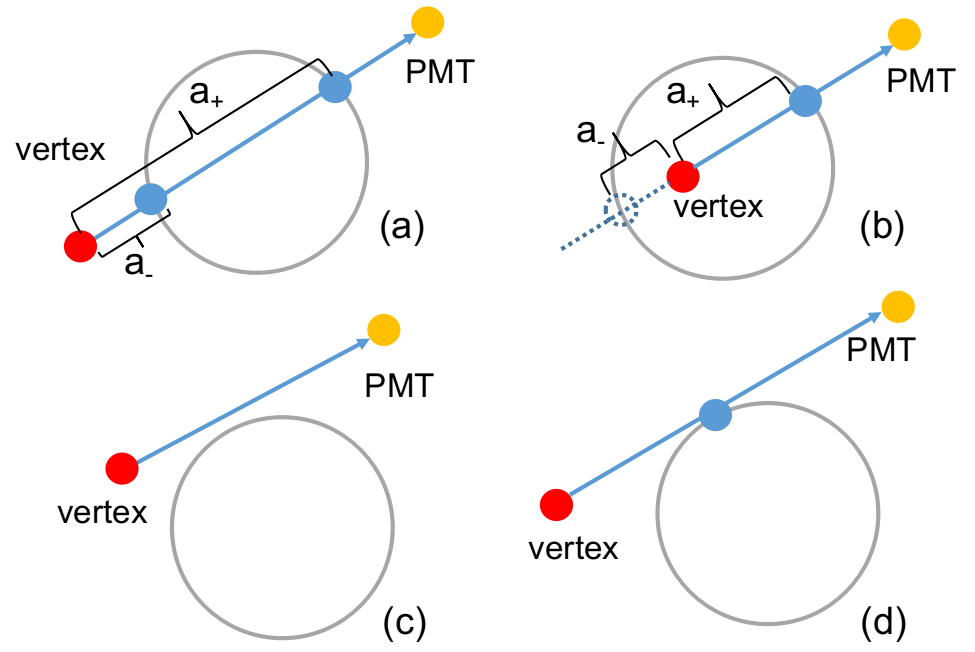
\includegraphics[width=80mm]{line-sphere.png}}
\caption[Line-sphere intersections.]{Line-sphere intersections. (a) the ray vector intersects the sphere with 2 points; (b) the ray vector intersects the sphere with 1 point; (c) and (d): the ray vector never passes through the sphere.}\label{line-sphere}
\end{figure}

\item Ray-plane intersection

For a `ray-plane' intersection, the $z$ components of the intersection points on $\vec{l}_0$ satisfy the plane equation $z=Z_\mathrm{split}$, where $Z_\mathrm{split}$ is the water level, i.e., the $z$ position of the water-scintillator intersection. Thus the intersection equation is:
$l_{0,z}=Z_\mathrm{split}$, where $l_{0,z}=z_0+a\cdot u_z$.

If $u_z=z_\mathrm{PMT}-z_0=0$, the ray is parallel to the plane and never intersects the plane.

If $u_z\neq 0$, solve the intersection equation $l_{0,z}=Z_\mathrm{split}$, we have: $a=(Z_\mathrm{split}-z_0)/u_z$.
Let: 
\begin{equation}
a_3 \equiv a = \frac{(Z_\mathrm{split}-z_0)|\vec{X}_{\mathrm{PMT}}-\vec{X_0}|}{z_\mathrm{PMT}-z_0}~~(if ~z_\mathrm{PMT}-z_0\neq 0),
\end{equation}

Similar to the case of ray-sphere intersection, if $a_3<0$, the ray-plane intersection point is on the extended line along the opposite direction to the ray; $a_3 \geq 0$ ensures the ray hits the interface. Note that here we consider the plane to be infinitely large: later we will combine with further logic to correct this fallacy. 

\item Ray-cylinder intersection

For a ray-cylinder intersection, the $x$ and $y$ components of the intersection points on $\vec l_0$ satisfy the intersection equation $l^2_{0,x}+l^2_{0,y} = r^2_\mathrm{neck}$, where $r_\mathrm{neck}$ is the radius of the neck cylinder ($r_\mathrm{neck}=785$~mm).

To solve the intersection equation, let 
\begin{equation*}
\Delta'\equiv [x_0\cdot (x_\mathrm{PMT}-x_0)+y_0\cdot(y_\mathrm{PMT}-y_0)]^2 - ( x_0^2+y_0^2-r^2_{neck})\cdot [(x_\mathrm{PMT}-x_0)^2+(y_\mathrm{PMT}-y_0)^2] \; . 
\end{equation*}
Then if $\Delta'>0$ we can solve for two roots, 
\begin{equation}\label{eq:ray-cylinder}
a'_{\pm} = |\vec{X}_\mathrm{PMT}-\vec{X}_0|\cdot\frac{-[x_0\cdot (x_\mathrm{PMT}-x_0)+y_0\cdot(y_\mathrm{PMT}-y_0)] \pm \sqrt{\Delta'} }{(x_\mathrm{PMT}-x_0)^2+(y_\mathrm{PMT}-y_0)^2} \; .
\end{equation}

Similar to the ray-sphere case, if $a'_{+} > a'_{-} > 0$, the length of the path inside the cylinder is $a'_{+} - a'_{-}$. In this case, the event position should be outside the cylinder, and the condition $(x^2_0+y^2_0)\geq r_\mathrm{neck}$ is automatically met. If $a'_+>0>a'_-$, the event position should be inside the cylinder and the ray-vector intersects the cylinder with one point (while the other point is along the opposite direction). Therefore, in this case the length of the path inside the cylinder is $a'_+$. If $\Delta'\leq0$, the ray vector never passes through the neck cylinder. Note that the calculations mentioned here assume that the cylinder is infinitely long ($-\infty<z<+\infty$). However, since the geometrical boundaries of the AV and PSUP are considered in the calculations, the fitter calculation in the neck region is only valid if $6000<z<8390$ mm (in the PSUP coordinates).

\end{itemize}

To evaluate the length ($d_{sp}$) of $|\vec{l}_p|$ that lies in the scintillator region, the above three geometrical criteria need to be combined carefully. The following two procedures go through all possible situations. First combine the evaluations of the ray-sphere and the ray-plane intersections to calculate the light path in the AV scintillator region ($d_{sp,\mathrm{AV}}$). Then combine the evaluations of the ray-sphere and the ray-cylinder intersections to calculate the light path in the neck scintillator region ($d_{sp,\mathrm{neck}}$). Detailed algorithms are shown in Appendix.~\ref{appendix:lightpath}.

Since a valid fit requires events to lie inside the PSUP sphere, only the part of the neck region that lies inside the PSUP sphere (with $6108<z_\mathrm{neck}<8390$~mm) needs to be considered. There is an option to turn off the neck path calculation, but if doing so a worse fit result is expected. Detailed calculations are shown in Appendix.~\ref{appendix:lightpath}.

If $d_{sp}=0$, the light path is entirely in water. In this case, the fitter is equivalent to the \texttt{MP water fitter}, and fits the vertex with the \texttt{MP water fitter} PDF. Once the light path passes through the scintillator region, the fitter fits with a scintillator timing PDF, in which the PMT time response is adjusted to account for photon propagation time in scintillator, as shown in Fig.~\ref{partialpdf}.

\begin{figure}[htbp]
	\centering	
	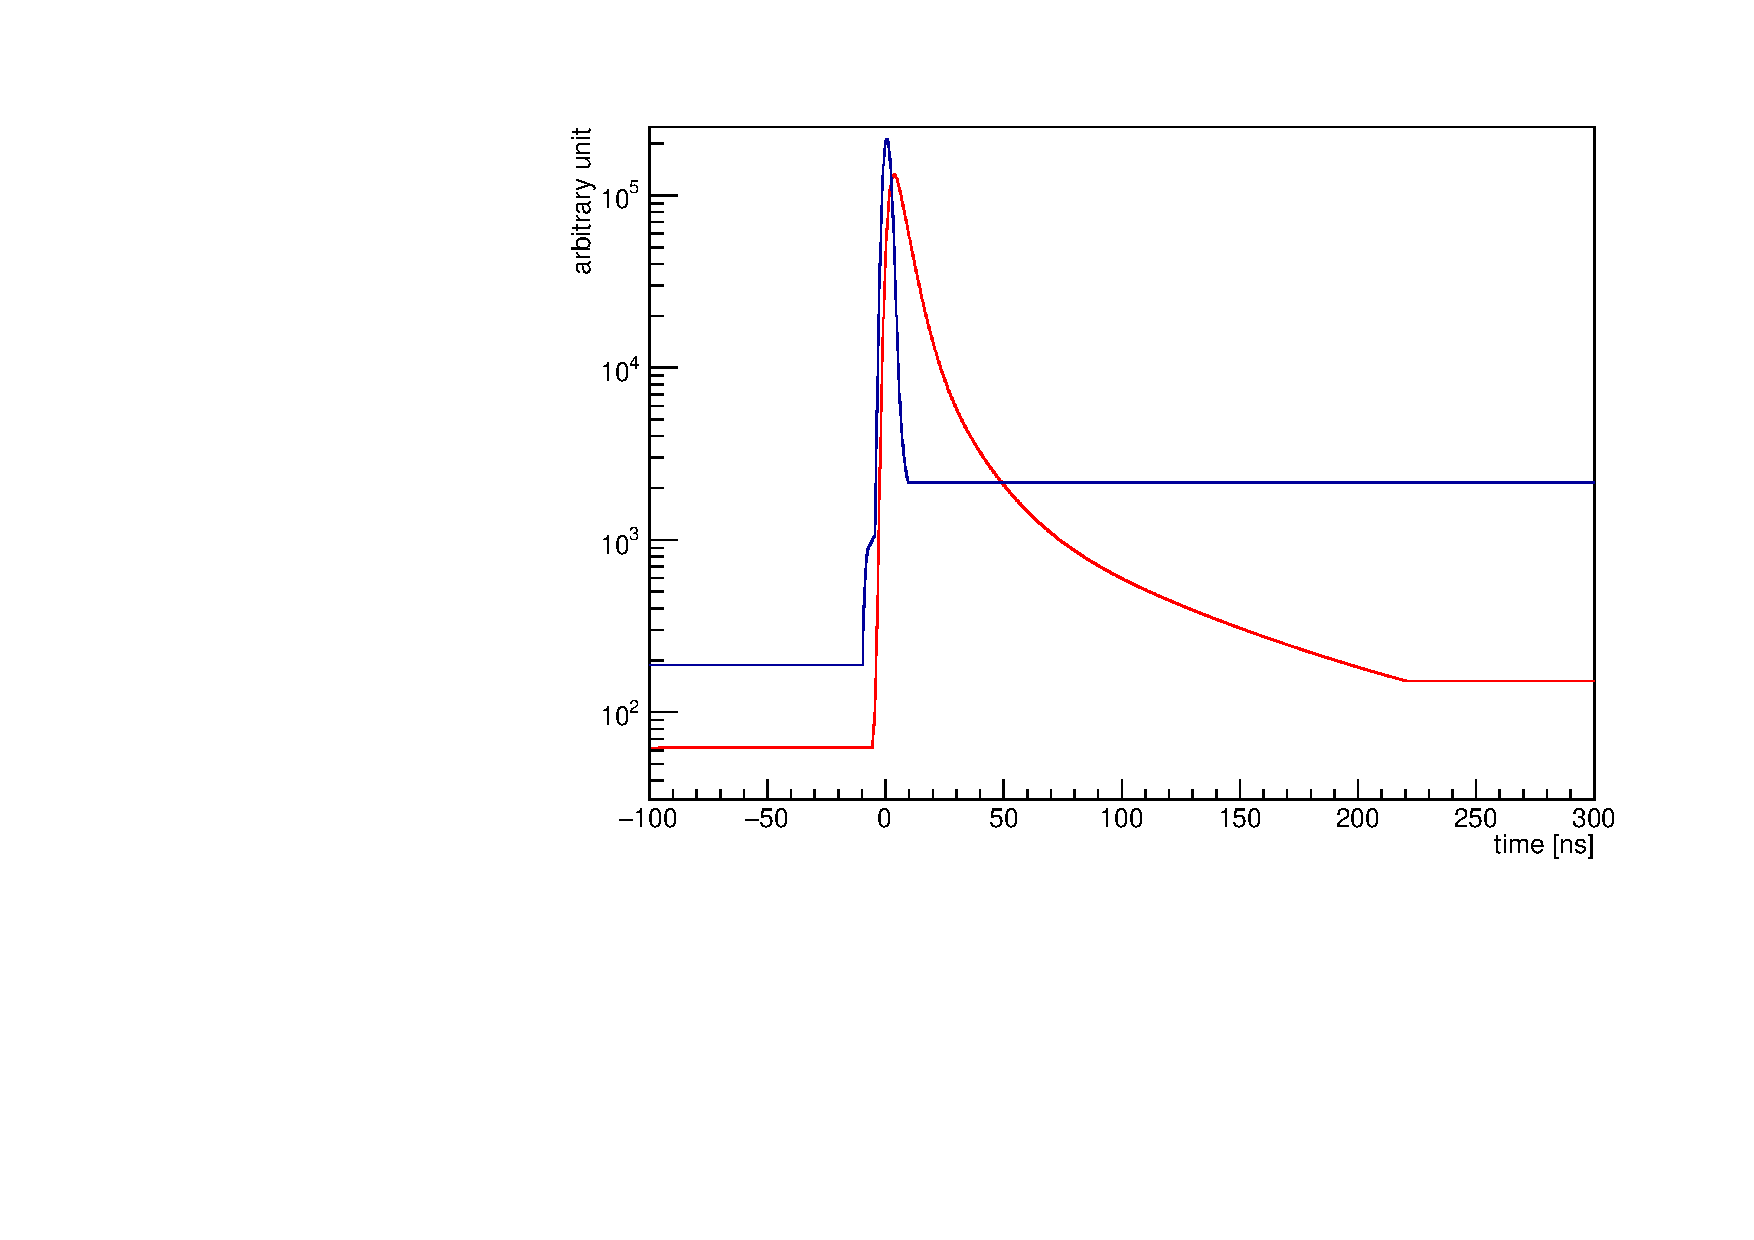
\includegraphics[width=7cm]{scintpdf.pdf}
	\caption[Timing PDFs used by the \texttt{MP scint-water fitter}.]{Timing PDFs used by the \texttt{MP scint-water fitter}. Blue: the timing PDF used by the \texttt{MPW fitter}; red: the scintillator timing PDF.	\label{partialpdf}}
\end{figure}

The next section will discuss the timing PDFs used by the fitter.

\subsection{Creating the Timing PDFs}

\subsubsection{Evolving PPO Concentration during the Filling}\label{sect:differentPPOconcen}

During the partial-fill phase, the water level and the concentration of the PPO were unsteady. PPO was gradually added into and mixed with the LAB, and during the relatively stable partial-fill stages, which (by virtue of that stability) were suitable for obtaining meaningful data to be analyzed, the PPO concentrations dissolved in the LAB were 0.25 g/L (earlier stage from 2019 to 2020) or 0.5 g/L (later stage from 2020 to 2021). The planned eventual concentration of the PPO in the scintillator phase is 2 g/L.

An understanding of the characteristic photon emission response is crucial for building the timing PDF for event reconstruction. The Oxford group from the SNO+ collaboration carried out bench-top measurements to obtain the time constants and relative light yields of an LAB sample carrying dissolved PPO at the following concentrations: 0.25, 0.5, 1.0, 2.0 and 6.0 g/L \cite{oxfordMeasurement0,oxfordMeasurement}.

The model used by the Oxford group to fit the emission time profile is \cite{oxfordMeasurement}: 
\begin{equation}
f_{optics}(t)= A' \; \frac{e^{-\frac{t}{\tau_{rise}}}}{\tau_{rise}} \, + \, \sum_{i=1}^3 (A_i\frac{e^{-\frac{t}{\tau_i}}-e^{-\frac{t}{\tau_{rise}}}}{\tau_i-\tau_{rise}}) \; ,
\end{equation}
where $A_i$ is the fraction of scintillation light emitted in the $i^{th}$ component of the detector medium, $A'$ is a small additional component with an instantaneous rise time and a
fall time equivalent to the rise time of the primary fluor to improve the fit quality with the measured data, $\tau_i$ is the corresponding decay constant, and $\tau_{rise}$ is the rise time of scintillator. The parameter values determined by the Oxford group from the bench-top experiments are listed in Table.~\ref{tab:measureAmplitude} and Table.~\ref{tab:measureLightYield}.

\begin{table}[ht]
	\centering\label{tab:measureAmplitude}
	\caption{\label{oxfordMeasure} Time constants and amplitudes measured by Ref.~\cite{oxfordMeasurement}. Here the relative light yield is with respect to the LAB+2 g/L PPO case (11900 photons/MeV).}	
	{\centering
		\begin{tabular*}{160mm}{c@{\extracolsep{\fill}}ccccccccc}
			\toprule 
			PPO [g/L] & $\tau_{rise}$ [ns] & $\tau_1$ [ns] & $\tau_2$ [ns] & $\tau_3$ [ns] & $A_1$ [\%]  & $A_2$ [\%]   & $A_3$ [\%]  & $A'$ [\%] \\
			\midrule
			0.25 & 1.25 & 8.1 & 25.0 & 68.2 & 29.2 & 53.1 & 13.9 & 3.8\\
			0.5  & 1.12 & 7.2 & 18.7 & 49.1 & 43.5 & 40.4 & 12.6 & 3.5 \\
			1.0 & 1.18 & 5.5 & 13.3 & 40.9 & 45.6 & 37.5 & 13.3 & 3.6 \\
			2.0 & 1.06 & 4.2 & 11.7 & 48.9 & 57.9 & 27.8 & 8.9 & 5.4	\\
			6.0 & 0.94 & 2.5 & 9.3  & 46.0 & 63.7 & 17.0 & 8.6 & 10.7\\
			\bottomrule	
		\end{tabular*}
	}
\end{table}

\begin{table}[ht]
	\centering\label{tab:measureLightYield}
	\caption{\label{oxfordMeasure2}Relative light yield (RLY) measured by Ref.~\cite{oxfordMeasurement}.}	
	{\centering
		\begin{tabular*}{60mm}{c@{\extracolsep{\fill}}cc}
			\toprule 
			PPO [g/L] & RLY \\
			\midrule
			0.25 & 0.57\\
			0.5 & 0.65\\
			1.0 & 0.9\\
			2.0 & 1.0\\
			6.0 & 0.93\\
			\bottomrule	
		\end{tabular*}
	}
\end{table}

These Oxford-measured time profiles were convolved with the PMT time response profile discussed in Sect.~\ref{sect:waterVertex}, Fig.~\ref{fig:MPW_timingPDF}, to obtain a timing PDF 
\begin{equation}\label{eq:OxfordTimingPDF}
f(t)_{PDF} = f_{optics}(t)\otimes f_{PMT~response}(t-t')
\end{equation}
for vertex reconstruction during the partial-fill. I wrote a python tool to create the timing PDFs to re-coordinate the partial fitter for the different PPO concentration cases \cite{partialFitterPDF}, as shown in Fig.~\ref{fig:oxfordPdf}\footnote{For other potential phases, the PDF can be built by using the timing spectrum described in Sect.~\ref{sect:LS_SNO+}.}.
\begin{figure}[!htb]
	\centering
	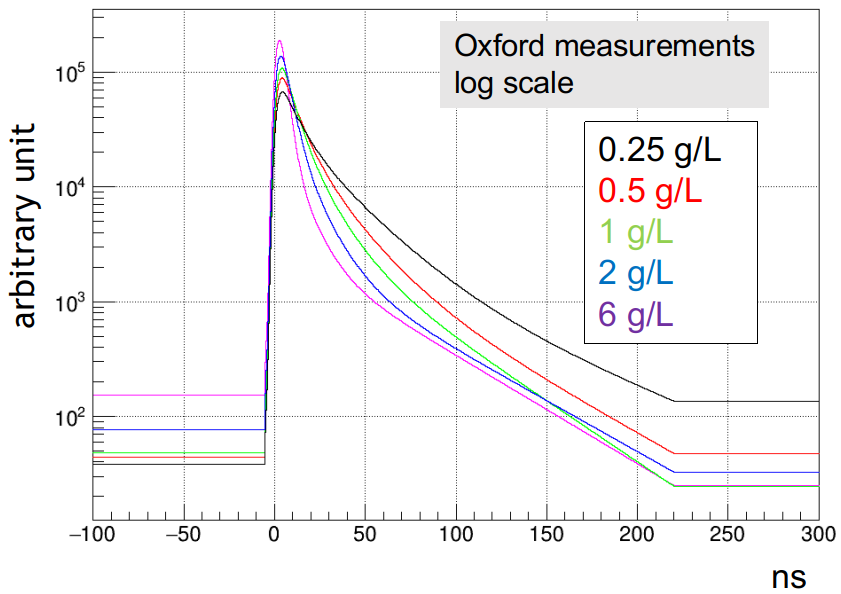
\includegraphics[width=10cm]{oxfordPdf_log.png}
	\caption{Timing PDFs built for various PPO concentrations based on the Oxford bench-top measurements.}
	\label{fig:oxfordPdf}
\end{figure}

Following the same method as was used for tuning $v_\mathrm{gr,eff}$ (see Sect.~\ref{sect:tuneGroupVelocity}), the effective group velocity in scintillator ($v_\mathrm{gr,scint}$) was obtained on the basis of simulations of 500 3 MeV electrons generated uniformly and with isotropic direction in the full scintillator geometry. The \texttt{MP scint fitter}, which will be discussed in Sect.~\ref{sect:scintFitter}, was used to reconstruct the same simulation data with different values of $v_\mathrm{gr}$. Once $v_\mathrm{gr,scint}$ was obtained, it was fixed in the \texttt{MP scint-water fitter}. Then $v_\mathrm{gr,water}$ was tuned by simulating five hundred 3 MeV electron events in the water region of the partial-fill geometry, with the water level set at z = 3000 mm in the AV coordinate. Fig.~\ref{fig:scint_groupVelocity} shows the convergence of the values of (a) $v_\mathrm{gr,scint}$ and (b) $v_\mathrm{gr,water}$ to their optimal values, from a linear interpolation in the LAB+0.5 g/L PPO scintillator case. Table.~\ref{partial_groupV} lists the effective group velocities and refractive indices ($n_\mathrm{eff}$) for the liquid scintillator with different PPO concentrations. 
		
\begin{figure}[htbp]
		\caption[Tuning the effective group velocities in the scintillator and water.]{Tuning the effective group velocities in the scintillator (a) and water (b).\label{fig:scint_groupVelocity}}
	\subfigure[Tuning the $v_\mathrm{gr,scint}$.]{
		\begin{minipage}[t]{0.4\textwidth}
		\centering
			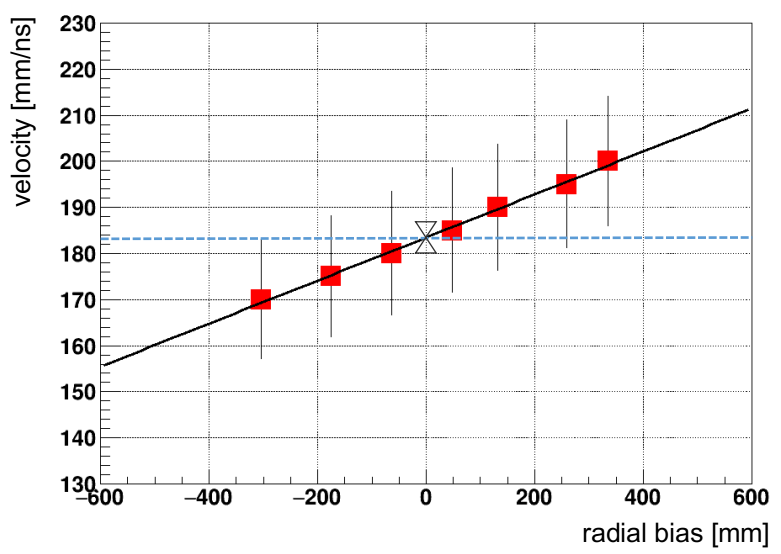
\includegraphics[width=6.5cm]{tune_groupVelocity_scint.png}
		\end{minipage}
	}   
	\subfigure[Tuning the $v_\mathrm{gr,water}$.]{ 
		\begin{minipage}[t]{0.4\textwidth}
			\centering
			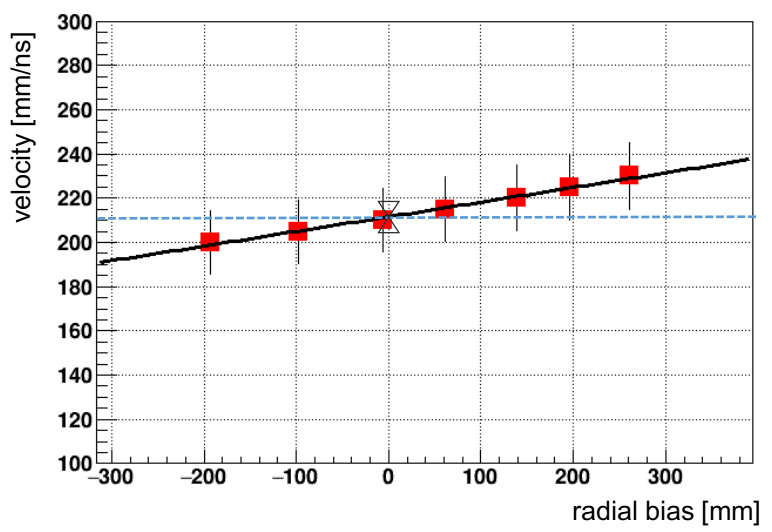
\includegraphics[width=6.5cm]{tune_groupVelocity_water.png}
		\end{minipage}
	}
\end{figure}

\begin{table}[ht]
	\centering
	\caption{\label{partial_groupV}Tuned effective group velocities for different PPO concentrations.}	
	{\centering
		\begin{tabular*}{140mm}{c@{\extracolsep{\fill}}ccccc}
			\toprule 
			PPO [g/L] & $V_{gr,scint}$ [mm/ns]& $n_\mathrm{eff,scint}$ & $V_{gr,water}$ [mm/ns]& $n_\mathrm{eff,water}$\\
			\midrule
			0.25 & 184.068$\pm$5.153 & 1.629 & 211.871$\pm$5.731 & 1.415\\
			0.5  & 183.467$\pm$5.159 &1.634& 211.587$\pm$-5.773 & 1.417 \\
			1.0 & 182.93$\pm$5.193 &1.639& 211.393$\pm$5.805& 1.418 \\
			2.0 & 183.045$\pm$5.184& 1.638& 211.629$\pm$5.767 & 1.417	\\
			6.0 & 184.218$\pm$5.135& 1.627& 211.173$\pm$5.843 &1.420\\
			\bottomrule	
		\end{tabular*}
	}
\end{table}

\subsection{Partial Fitter Performance}

The performance of the \texttt{MP scint-water fitter} was studied with MC simulations. During the partial-fill phase, the filling and mixing of the liquid scintillator was stable at several water levels for data taking and data analysis. A typical water level is 3 m from the AV bottom, and a typical PPO concentration is 0.5 g/L. With these two settings in the partial-fill geometry, to test the partial fitter's performance 5000  electron events (3 MeV, uniform in position, isotropic in direction) were simulated in each of the regions, i.e. scintillator region and water region.

The average fit speed for vertex reconstruction of events in the scintillator region proved to be 0.2 second/event, which is acceptable for the data processing during the partial-fill phase. For the events in the water region, the average fit speed was 0.05 s/event, which is similar to the value yielded by the \texttt{MPW fitter}. Fig.~\ref{fig:partial_inScint} and Fig.~\ref{fig:partial_inWater} show the results of the \texttt{MP scint-water fitter} reconstructed positions in the scintillator and water regions respectively. The subfigures (a) are the reconstructed positions projected onto the ($\sqrt{x^2+y^2}$, $z$) plane while the subfigures (b), (c) and (d) are the position biases between the reconstruction and MC truth, projected onto the ($x,y,z$)-axes respectively. The distributions of the position bias were fitted with Gaussian functions and the values of the Gaussian mean ($\mu_{x,y,z}$) and standard deviation ($\sigma_{x,y,z}$) quantify fit bias and resolution.

\begin{figure}[htbp]\setcounter{subfigure}{0}
	\centering
	\subfigure[$\rho=\sqrt{x_{fit}^2+y_{fit}^2}$ vs. $z_{fit}$.]
	{ 
		\begin{minipage}[b]{0.38\textwidth}
			\centering
			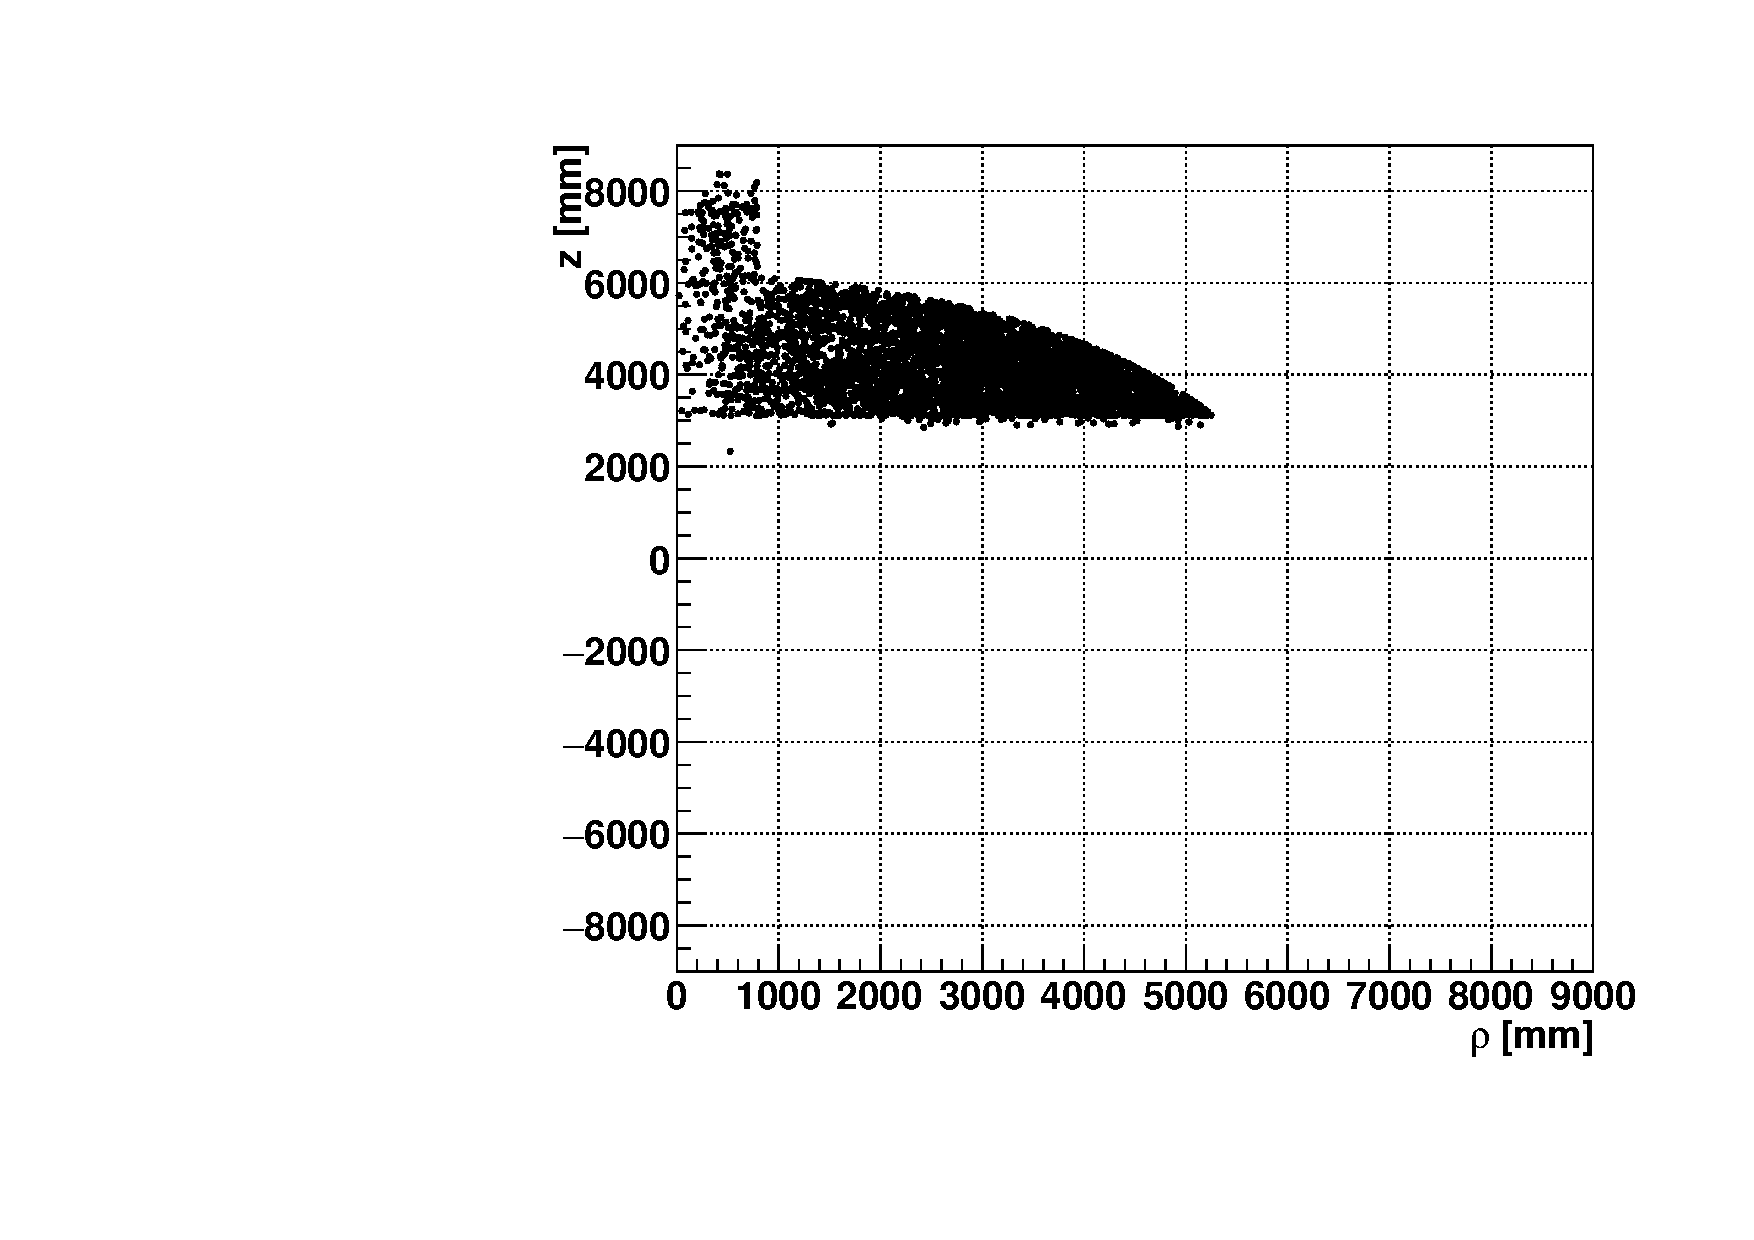
\includegraphics[width=6.5cm]{partial_top_3MeV_rhoVsZ.pdf}
		\end{minipage}
	}
	\subfigure[$x_{fit}-x_{mc}$.]{
		\begin{minipage}[t]{0.38\textwidth}
			\centering
			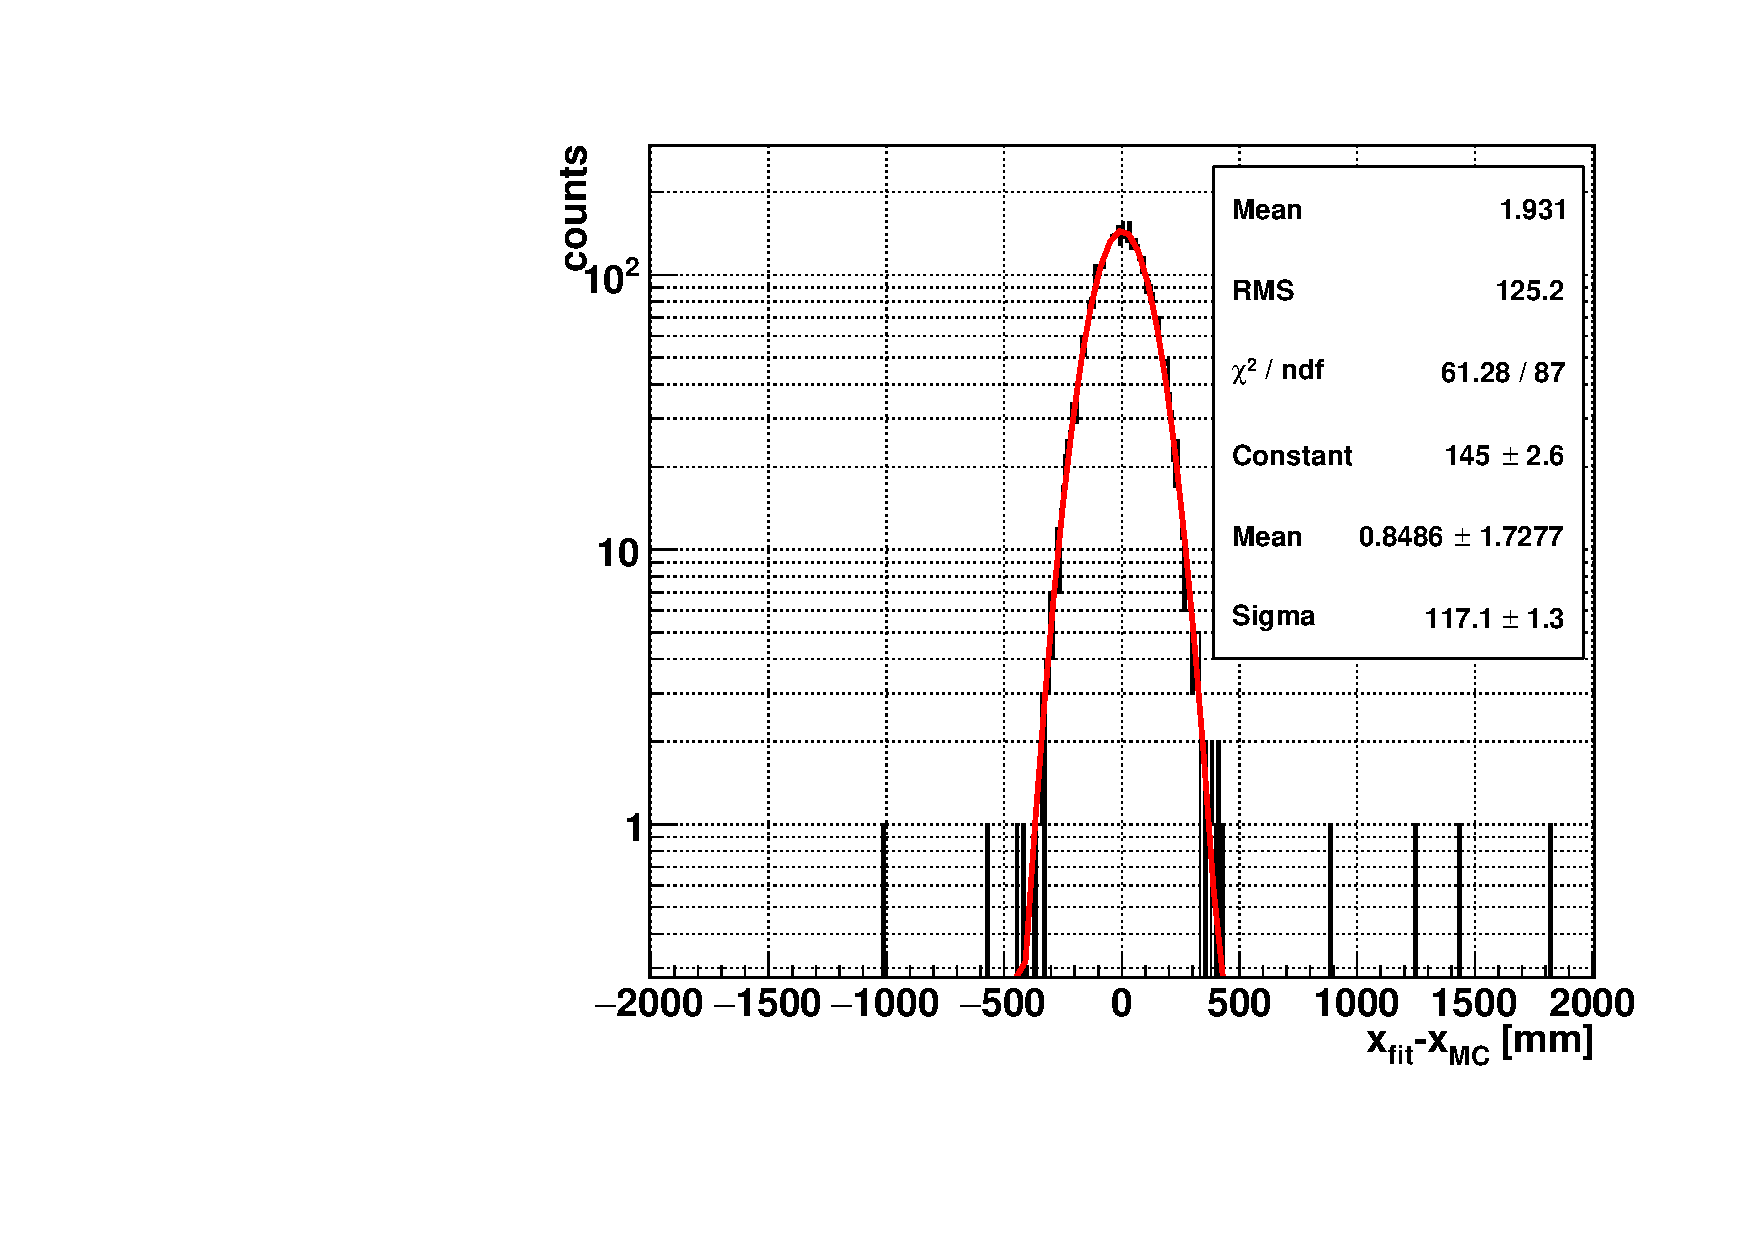
\includegraphics[width=6.5cm]{partial_top_3MeV_xbias.pdf}
		\end{minipage}
	}   
	\subfigure[$y_{fit}-y_{mc}$.]{
		\begin{minipage}[t]{0.38\textwidth}
			\centering
			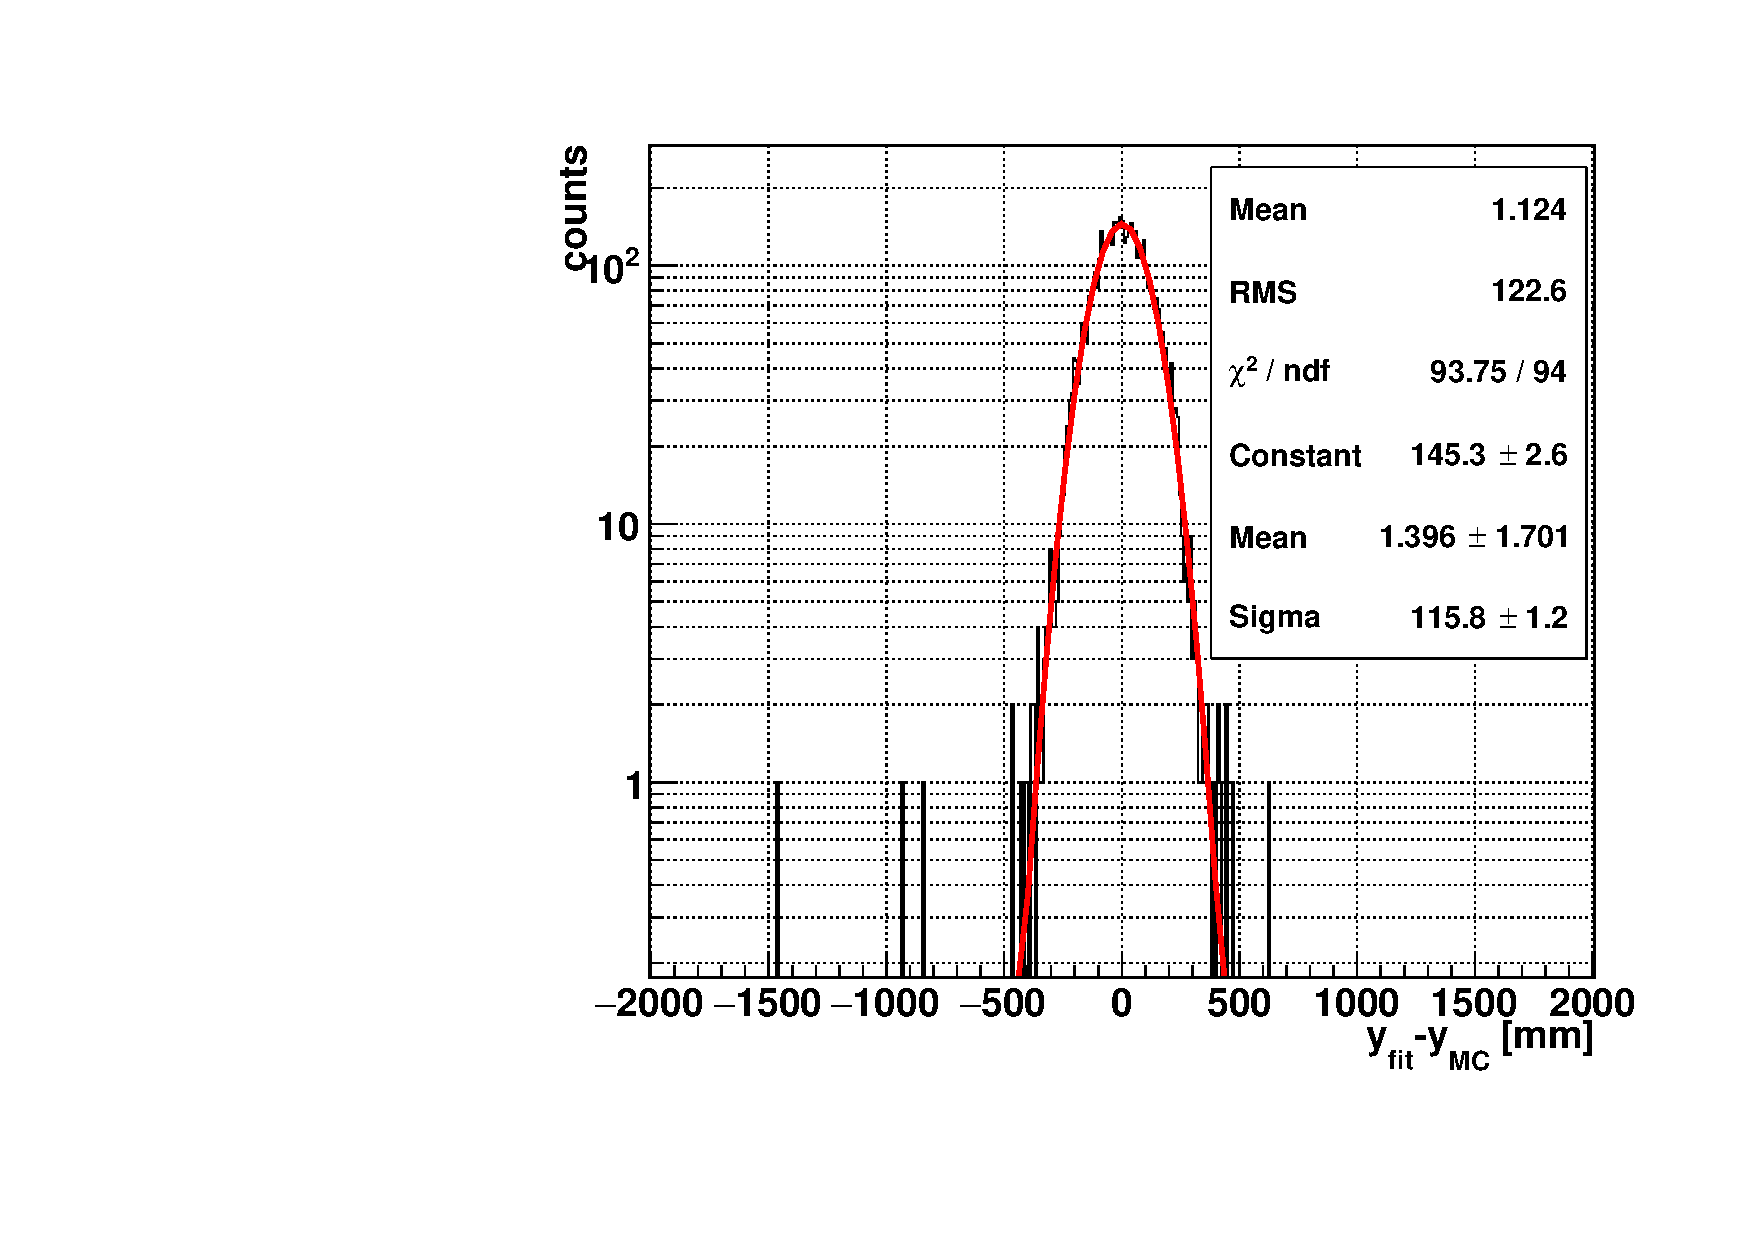
\includegraphics[width=6.5cm]{partial_top_3MeV_ybias.pdf}
		\end{minipage}
	}
	\subfigure[$z_{fit}-z_{mc}$.]{
		\begin{minipage}[b]{0.38\textwidth}
			\centering
			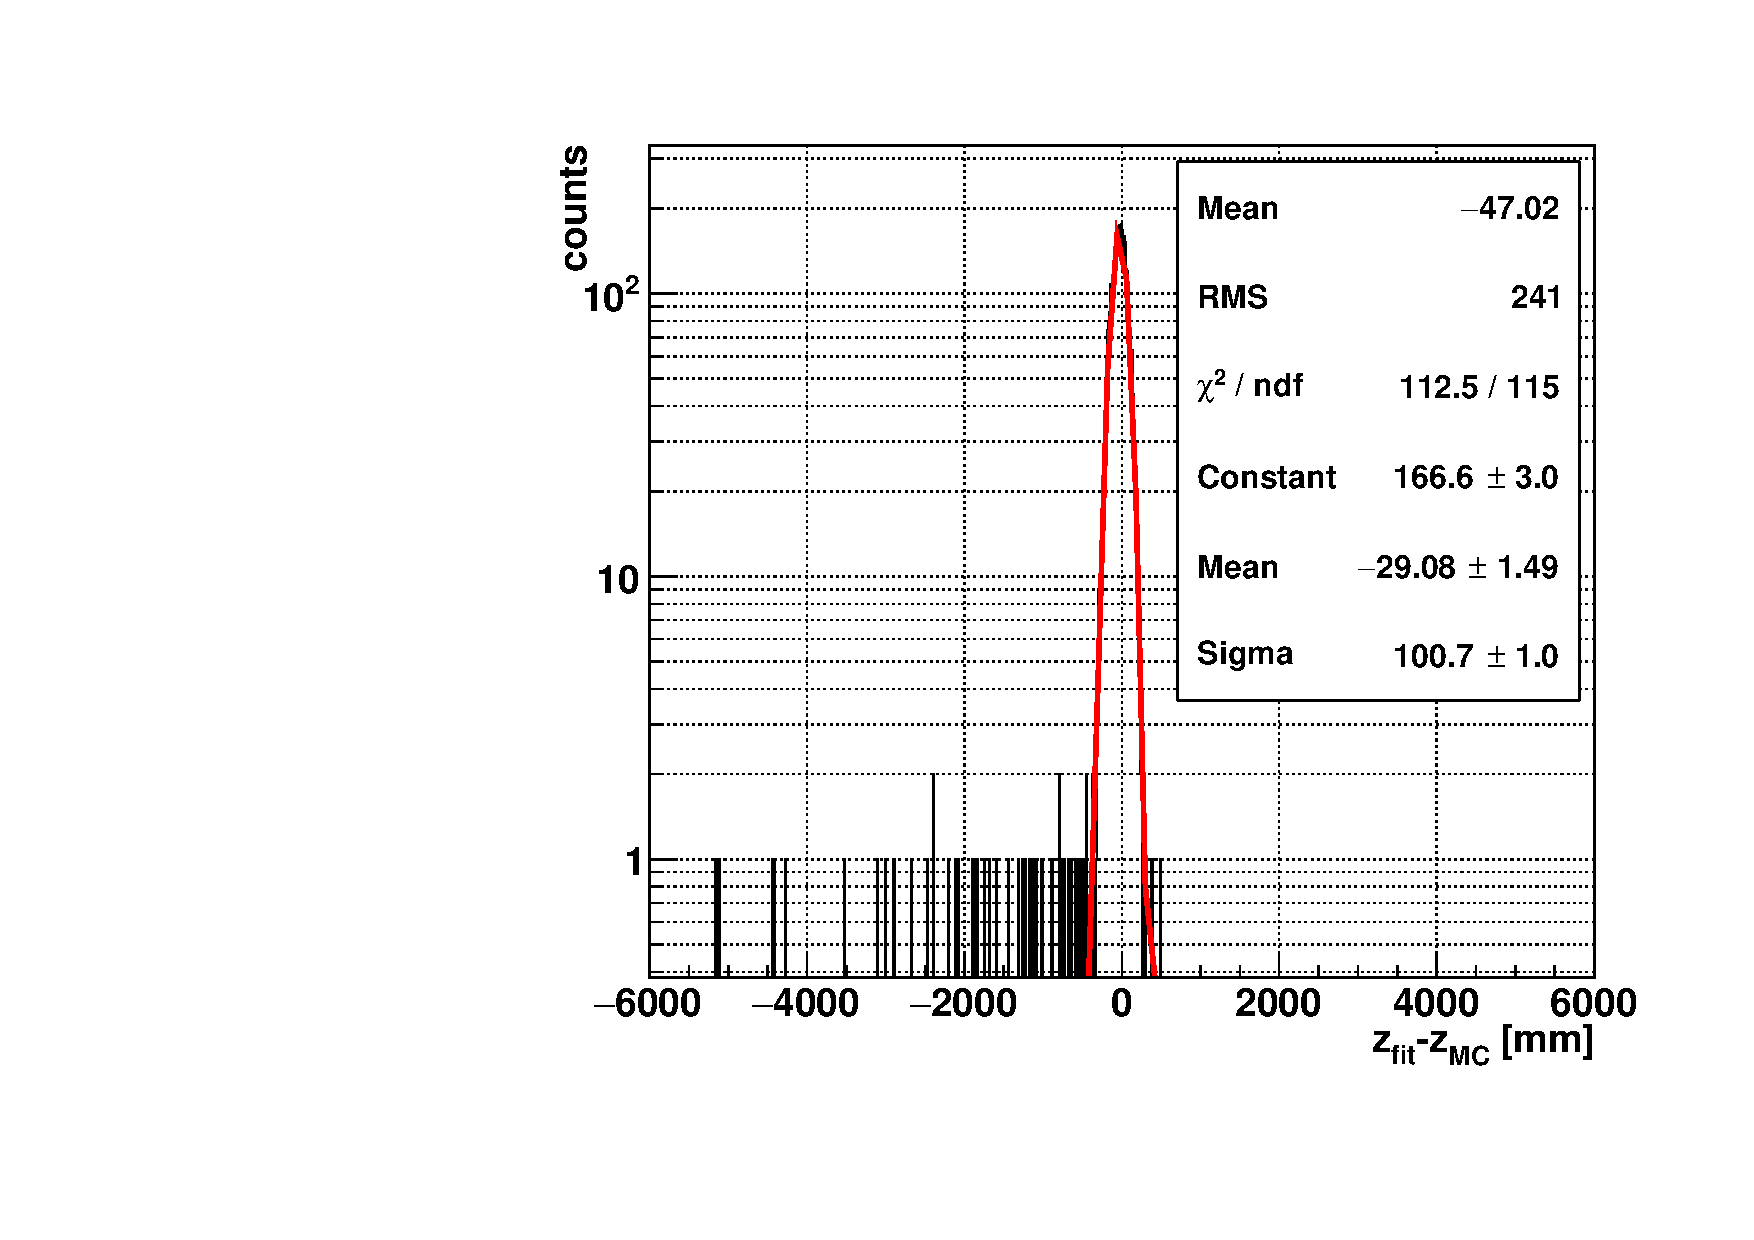
\includegraphics[width=6.5cm]{partial_top_3MeV_zbias.pdf}
		\end{minipage}
	}
	\caption{Reconstructed position and fit bias for simulated 3 MeV electron events in the scintillator region.\label{fig:partial_inScint}}
\end{figure}

Fig.~\ref{fig:partial_inScint} shows that for events in the scintillator region, the resolutions $\sigma_{x,y,z}$ are all better than 150 mm. The biases on $x$ and $y$ axes ($\mu_{x,y}$) are smaller than 1.5 mm, while the bias $\mu_z$ along $z$ is significantly larger, about -29 mm. The larger bias in $z$ is mostly caused by events that are mis-reconstructed in the water region. The main reason for that mis-reconstruction is caused by the fitter omitting the calculations relating to reflection and refraction of light paths happening at the water-scintillator interface or at AV boundaries, as earlier mentioned. Since the refractive index of the liquid scintillator exceeds that of water, some photons are reflected off the water-scintillator interface. The reflection results in a light path with a longer $t_\mathrm{transit}$, but the event is still created in the scintillator region. While the fitter does properly handle the reflected light path, it will pull the event into the water region a little further from the actual position to ``explain'' the longer $t_\mathrm{transit}$, causing the event to be mis-reconstructed in the water region. This explains the mis-reconstructed events with $z_{fit}-z_{MC}<0$ in Fig.~\ref{fig:partial_inScint} (d). Sect.~\ref{sect:partialFitterDiscuss} will discuss improving the fitter. Some of these mis-reconstructed events can be removed by applying the $posFoM$ cut. 

Fig.~\ref{fig:partial_scaleLogLcut} (a) shows the (vertical) fit error $z_{fit}-z_{MC}$ versus the $posFoM$ quantity $scaleLogL$ mentioned in Sect.~\ref{sect:positionFoM}. Application of a $scaleLogL>9.8$ cut removes more than a third of the mis-reconstructed events with $|\vec{X}_{fit}-\vec{X}_{MC}|>1000$ mm. In Fig.~\ref{fig:partial_scaleLogLcut} (b), the fit position bias in $z$ ($z_{fit}-z_{MC}$) after the cut is plotted in red, overlaid with the distribution before the cut in black. By fitting with the Gaussian function, it is evident that the cut removes some mis-reconstructed events on the tail of the distribution, improving the resolution by about 1.5 mm and reducing the bias by about 1.9 mm compared to the plot in Fig.~\ref{fig:partial_inScint} (d). As shown in Fig.~\ref{fig:partial_scaleLogLcut} (c), this cut removes most of the outliers observed in the $\rho$ vs $z$ plot in Fig.~\ref{fig:partial_inScint} (a).

\begin{figure}[htbp]
	\centering
	\subfigure[$z_{fit}-z_{MC}$ vs. $scaleLogL$.]{ 
		\begin{minipage}[b]{0.38\textwidth}
			\centering
			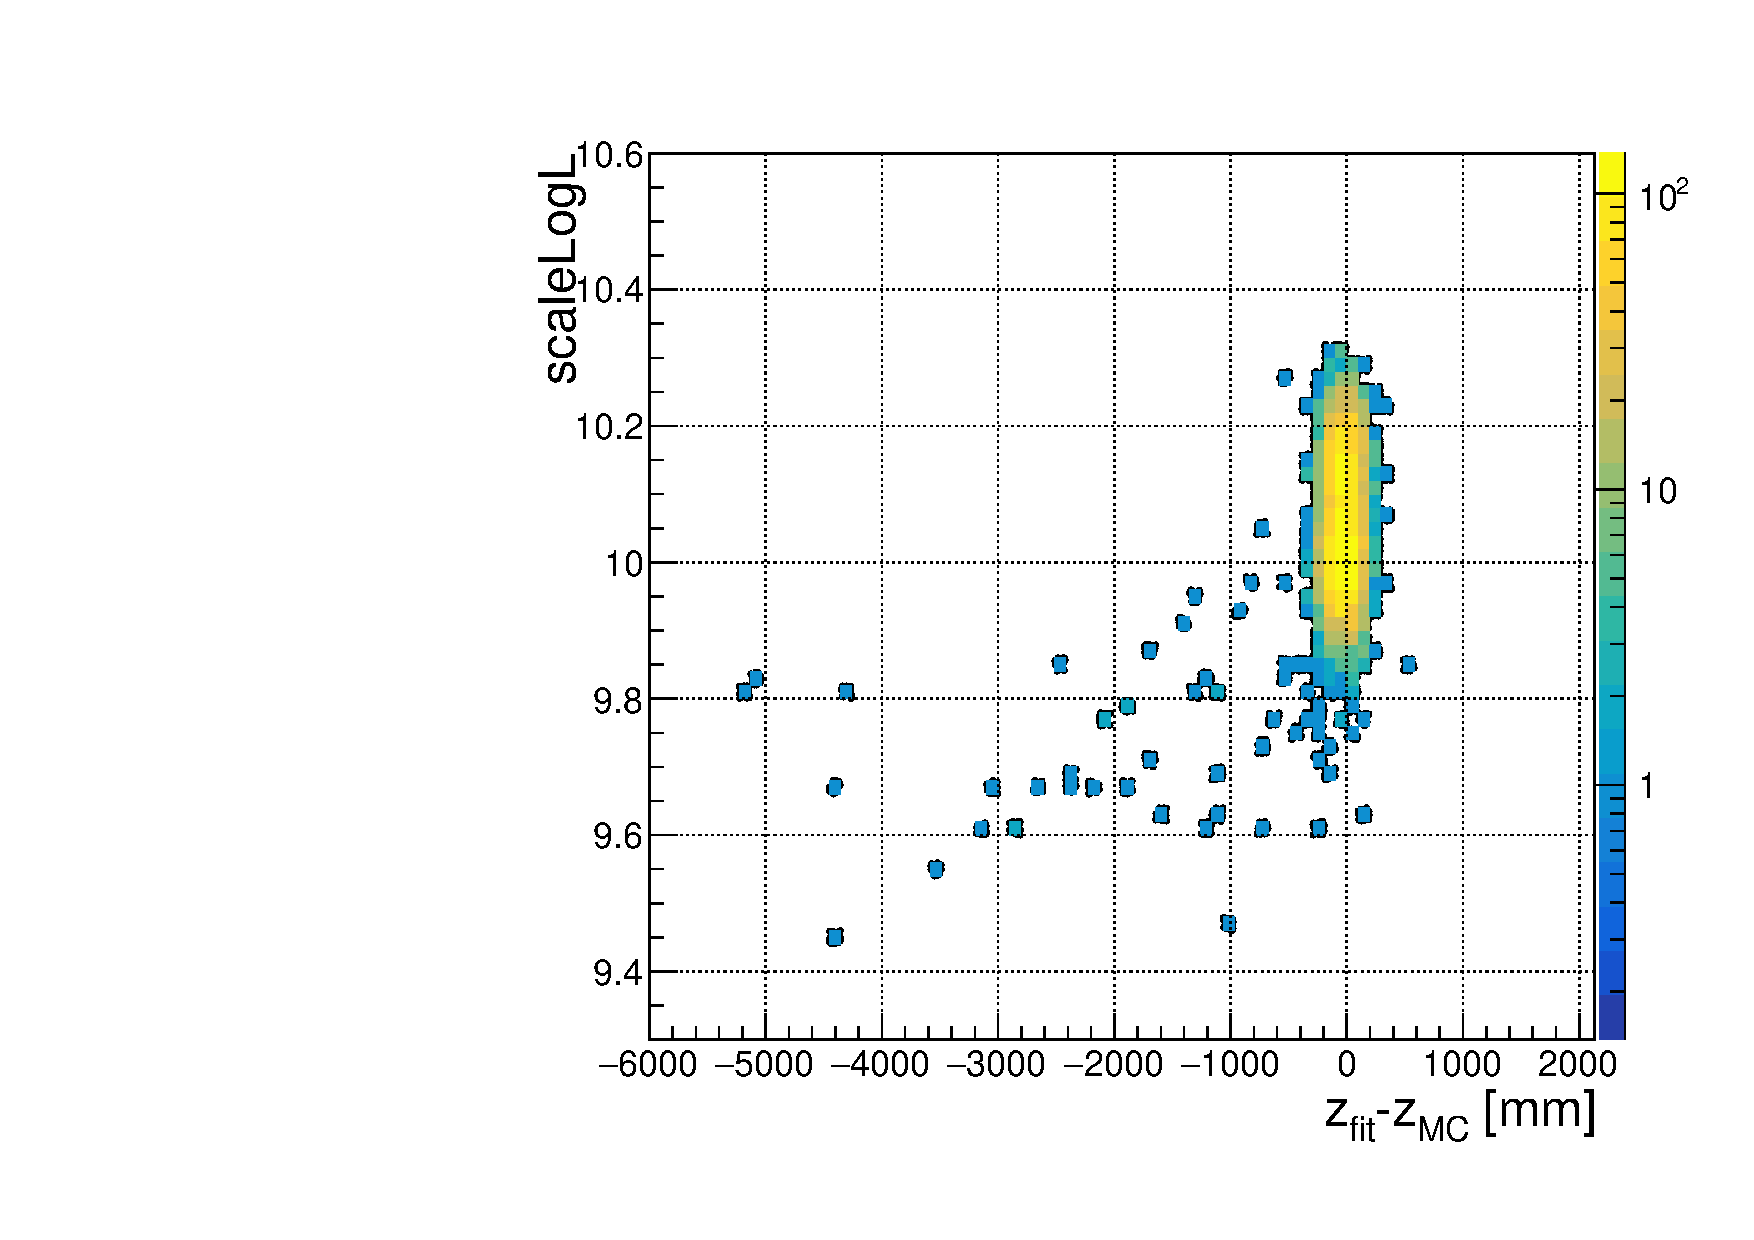
\includegraphics[width=6cm]{scaleLogLvsZbias_top.pdf}
		\end{minipage}
	}
	\subfigure[$z_{fit}-z_{mc}$, before (black) and after (red) the $scaleLogL>9.8$ cut.]{
		\begin{minipage}[t]{0.38\textwidth}
			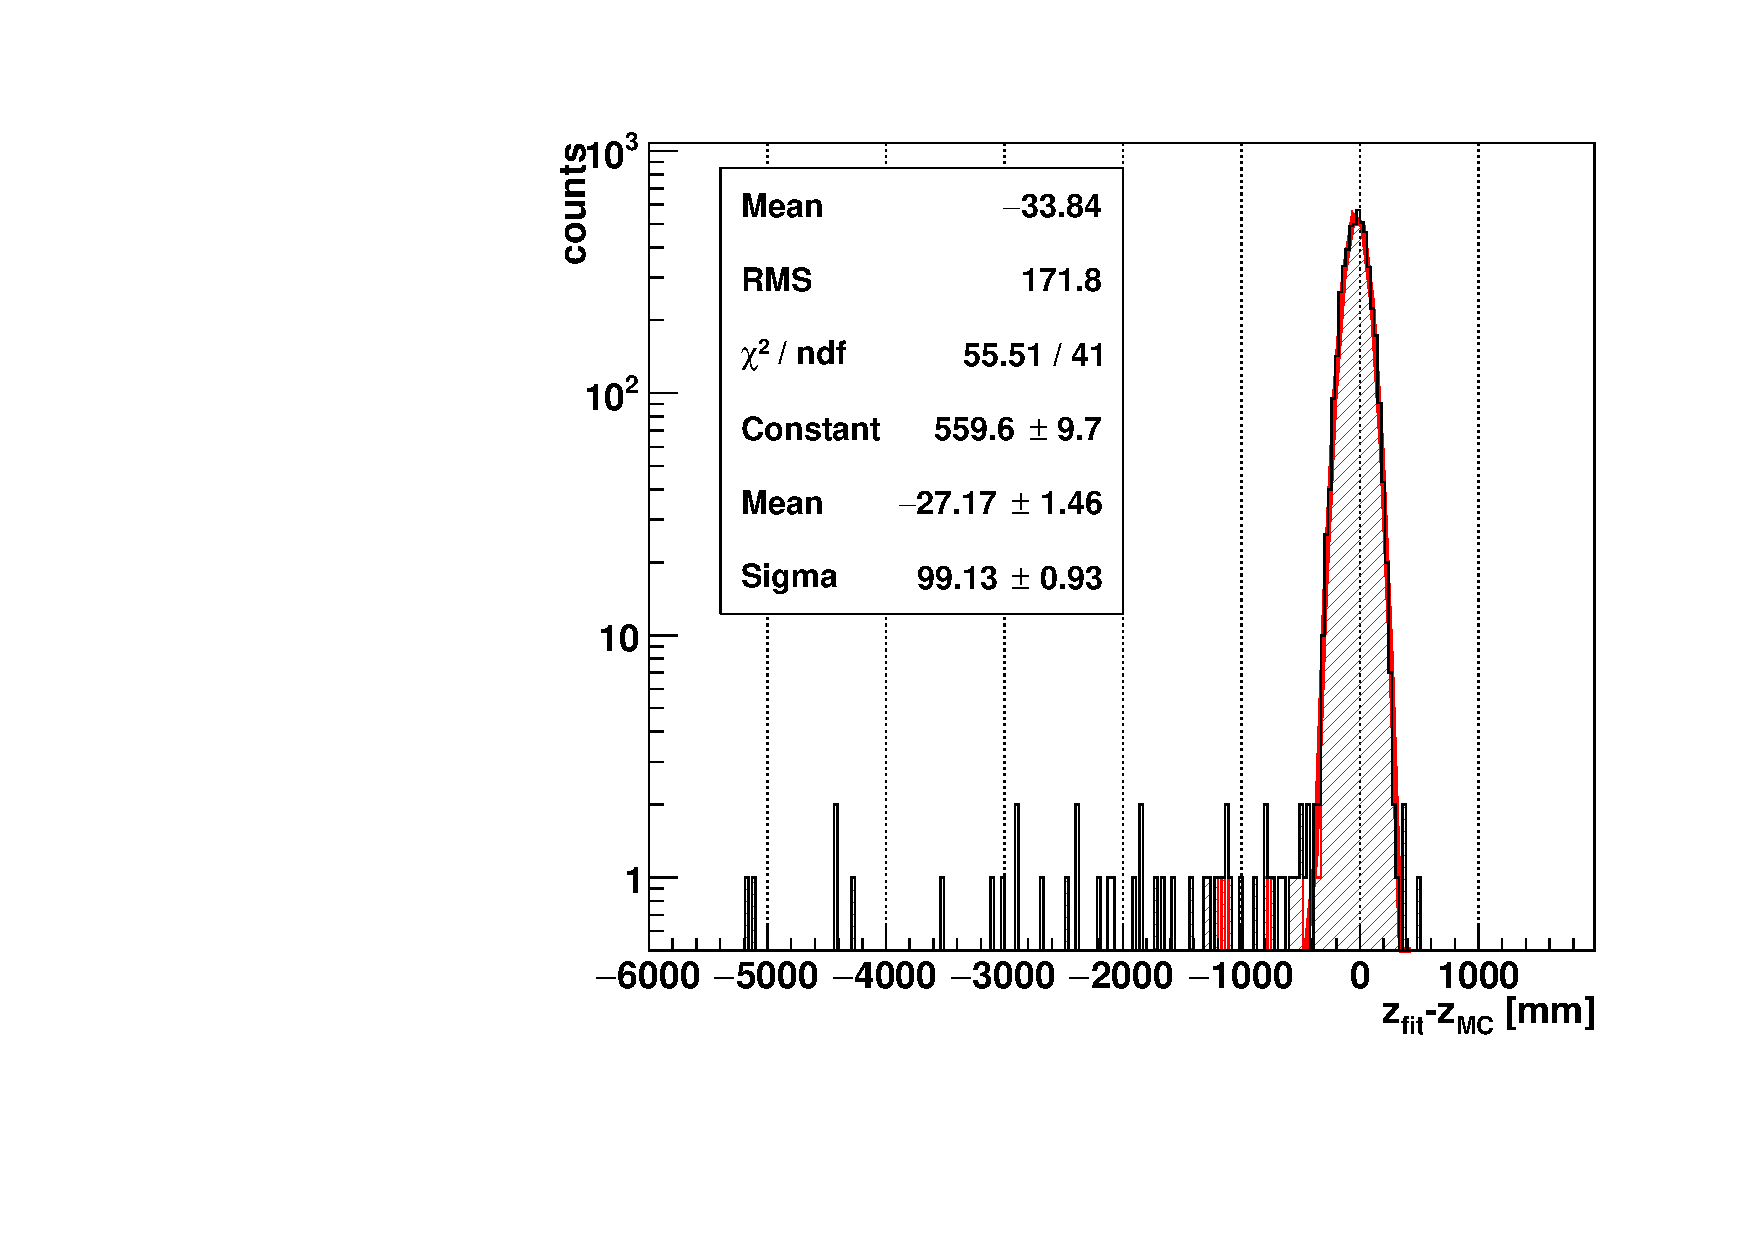
\includegraphics[width=6.5cm]{zbias_top_afterScaleLogLcut.pdf}
		\end{minipage}
	}   
	\subfigure[$\rho_{fit}$ vs. $z_{fit}$, with $scaleLogL>9.8$.]{ 
		\begin{minipage}[t]{0.38\textwidth}
			\centering
			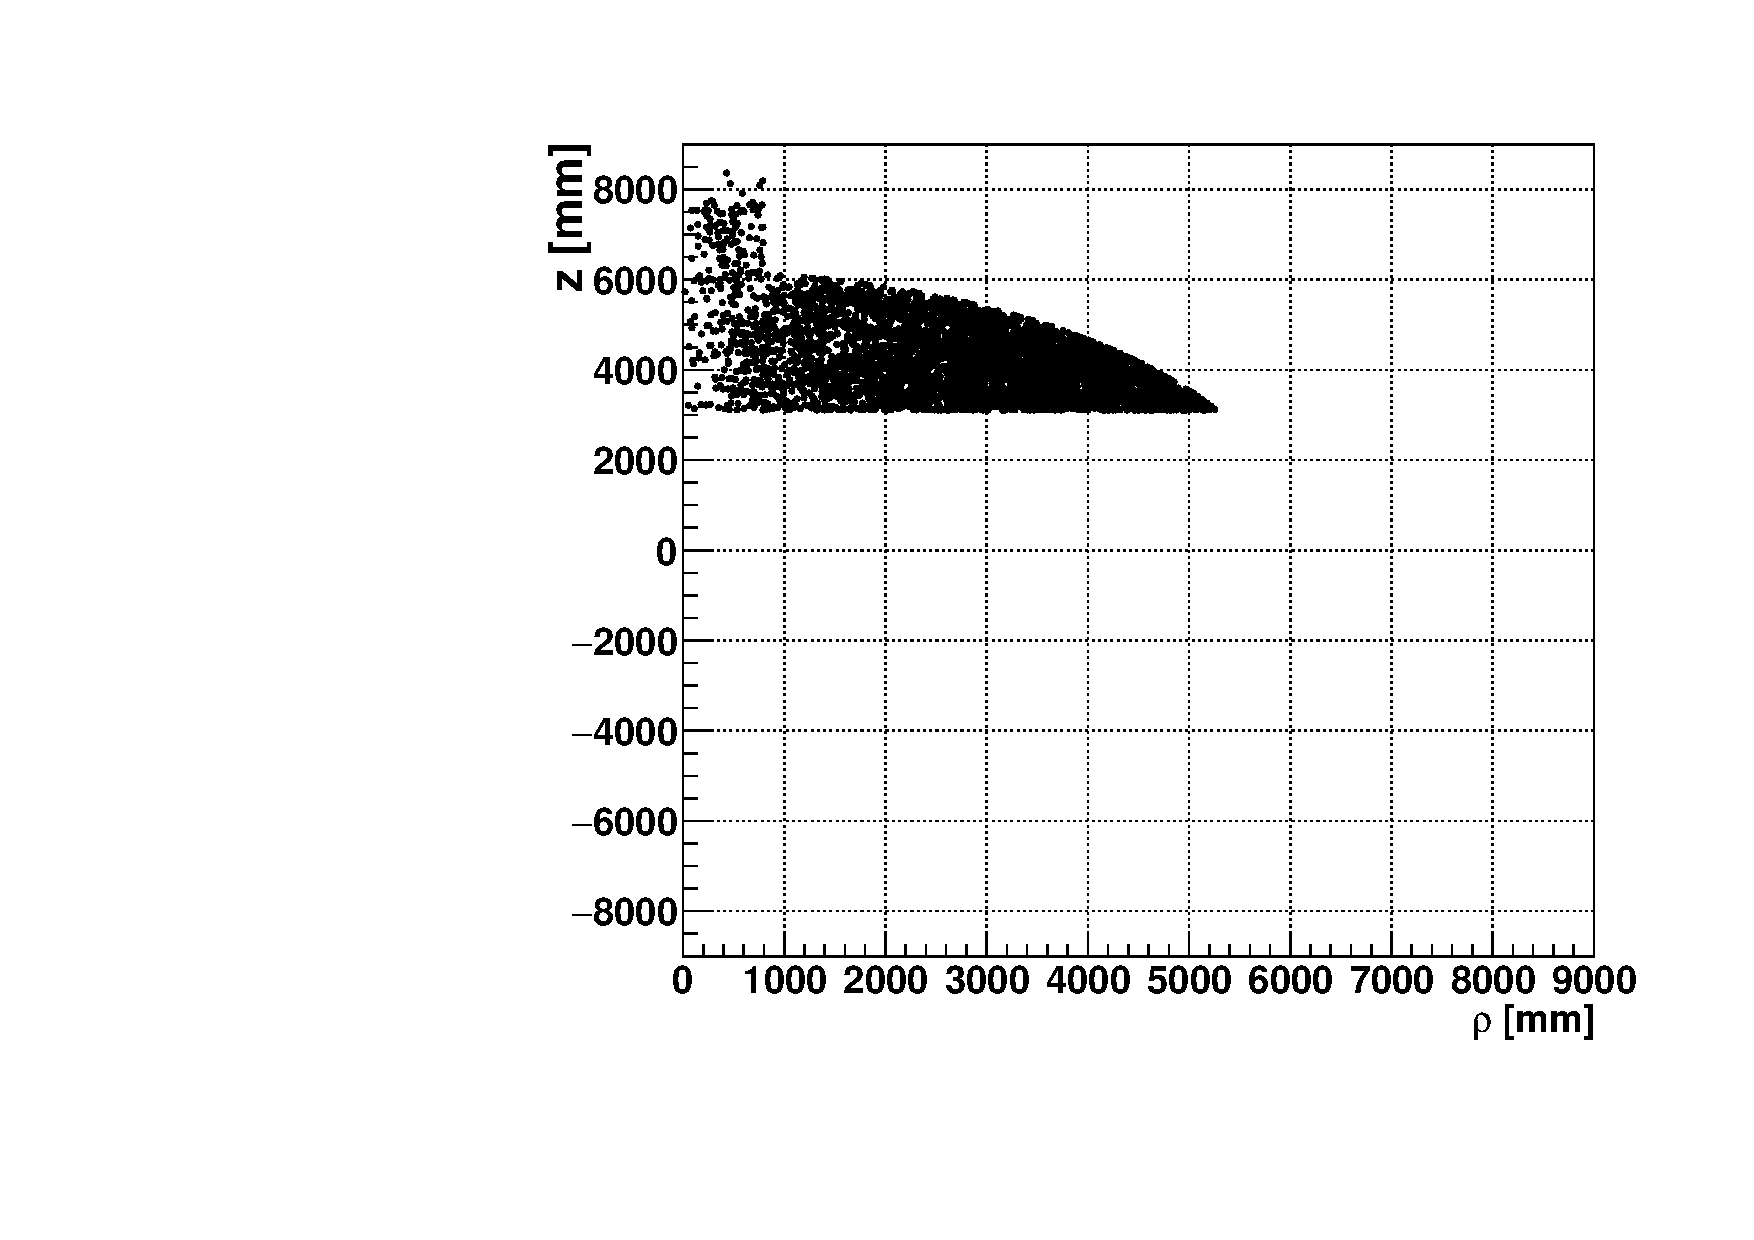
\includegraphics[width=6.5cm]{partial_top_scaleLogL9p8cut_3MeV_rhoVsZ.pdf}
		\end{minipage}
	}
	\caption{Effects of the $scaleLogL$ cut on the reconstructed positions and fit biases.\label{fig:partial_scaleLogLcut}}
\end{figure}

For events in the water region, the fit position biases in $x$ and $y$ ($\mu_{x,y}$) are comparable to the results of the \texttt{MPW fitter} shown in Sect.~\ref{sect:waterFitterVertex}, while $\mu_z$ is about 50 mm worse and the resolutions $\sigma_{x,y,z}$ are about 100 mm worse. This is due to the previously mentioned effects of the water-scintillator interface and boundaries. These boundary effects are more obvious (more severe) for events in the water than for those in the scintillator region, as shown by the $\rho$ vs. $z$ plot in Fig.~\ref{fig:partial_inWater} (a). This is due to the lower NHits (fewer triggered PMTs) of events in the water, providing less information for the fitter. However, the poorer reconstruction performance for water events is not significant for the partial-fill analysis: since the analysis is focused on studying the liquid scintillator, events in the water region are less interesting and are mostly removed by the NHits and fiducial volume cuts (NHits$>40$ was applied on the data processing during the partial-fill phase). 

\begin{figure}[htbp]
	\centering
	\subfigure[$\rho=\sqrt{x_{fit}^2+y_{fit}^2}$ vs. $z_{fit}$.]
	{ 
		\begin{minipage}[b]{0.38\textwidth}
			\centering
			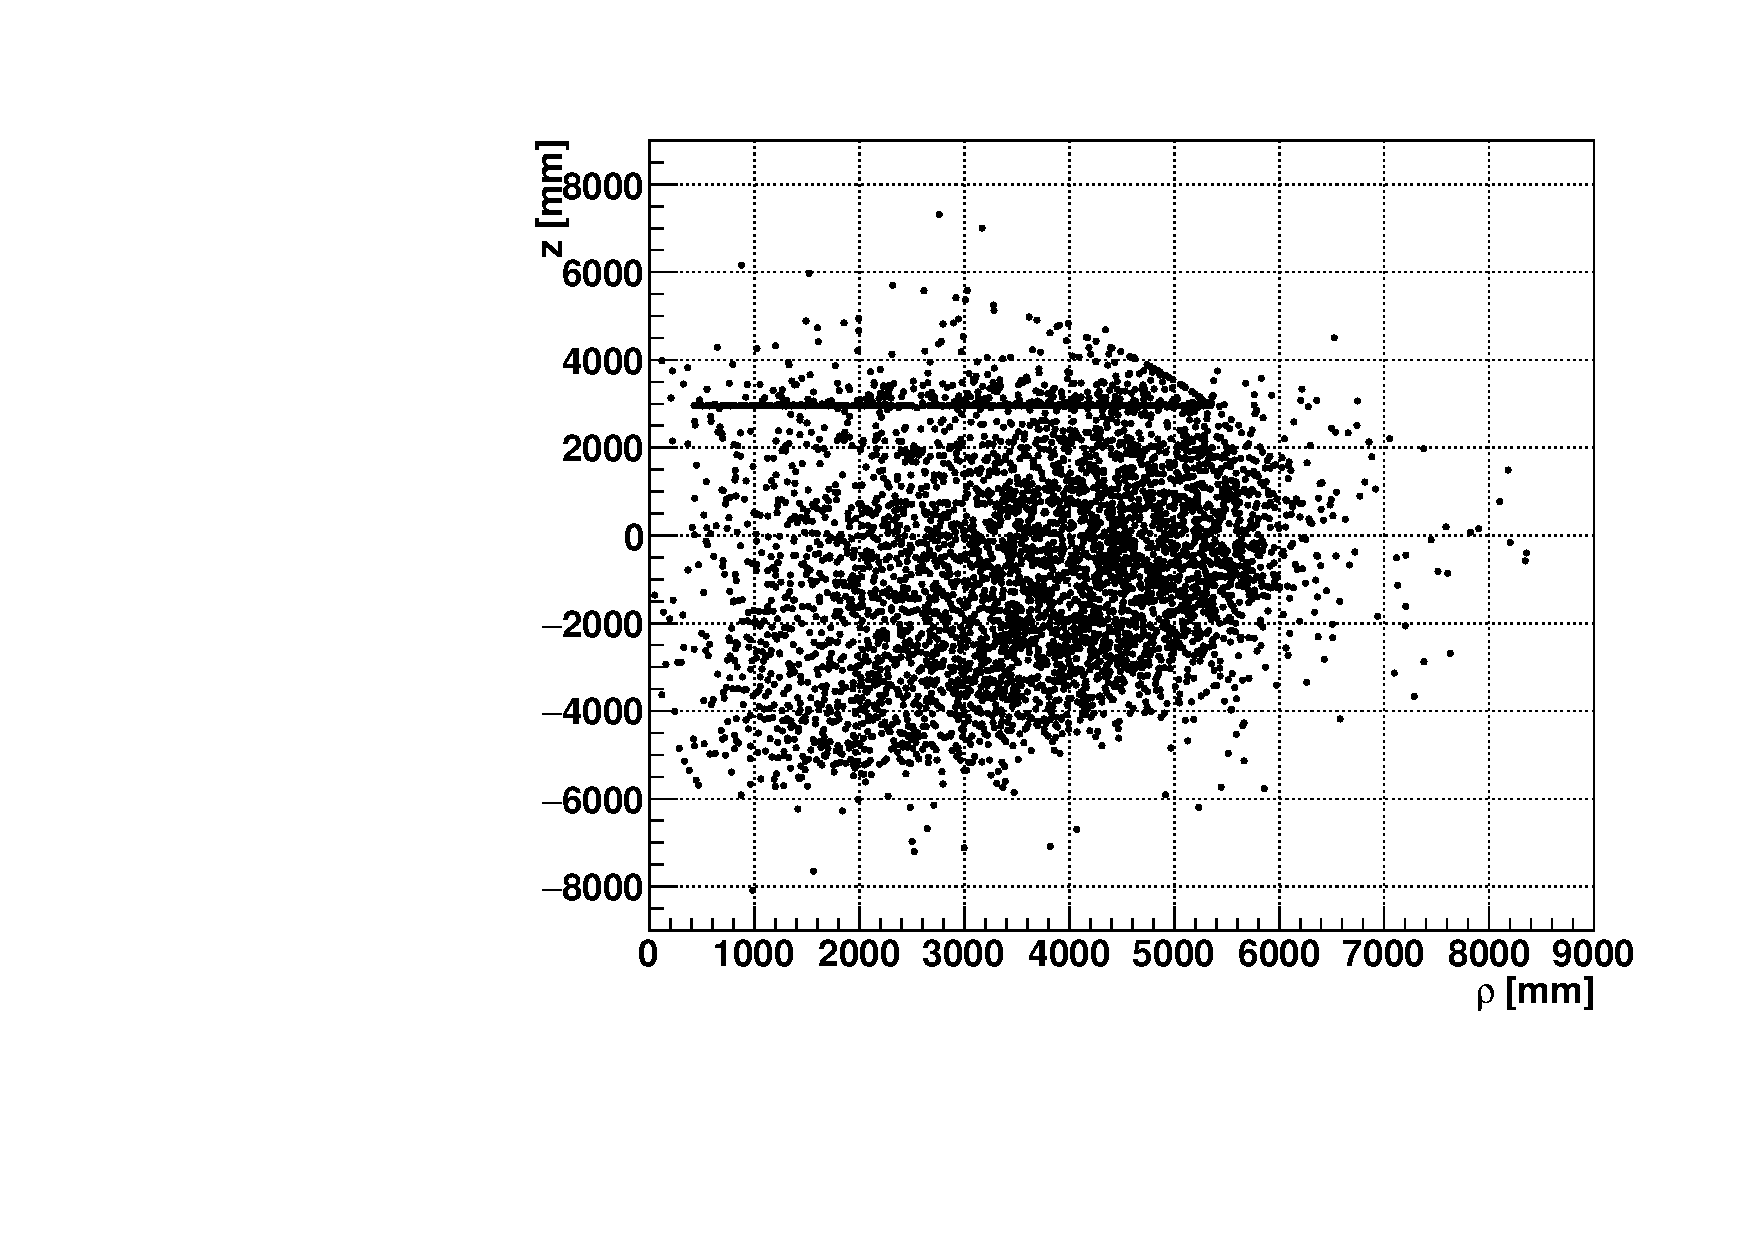
\includegraphics[width=6.5cm]{partial_bot_3MeV_rhoVsZ.pdf}
		\end{minipage}
	}
	\subfigure[$x_{fit}-x_{mc}$.]{
		\begin{minipage}[t]{0.38\textwidth}
			\centering
			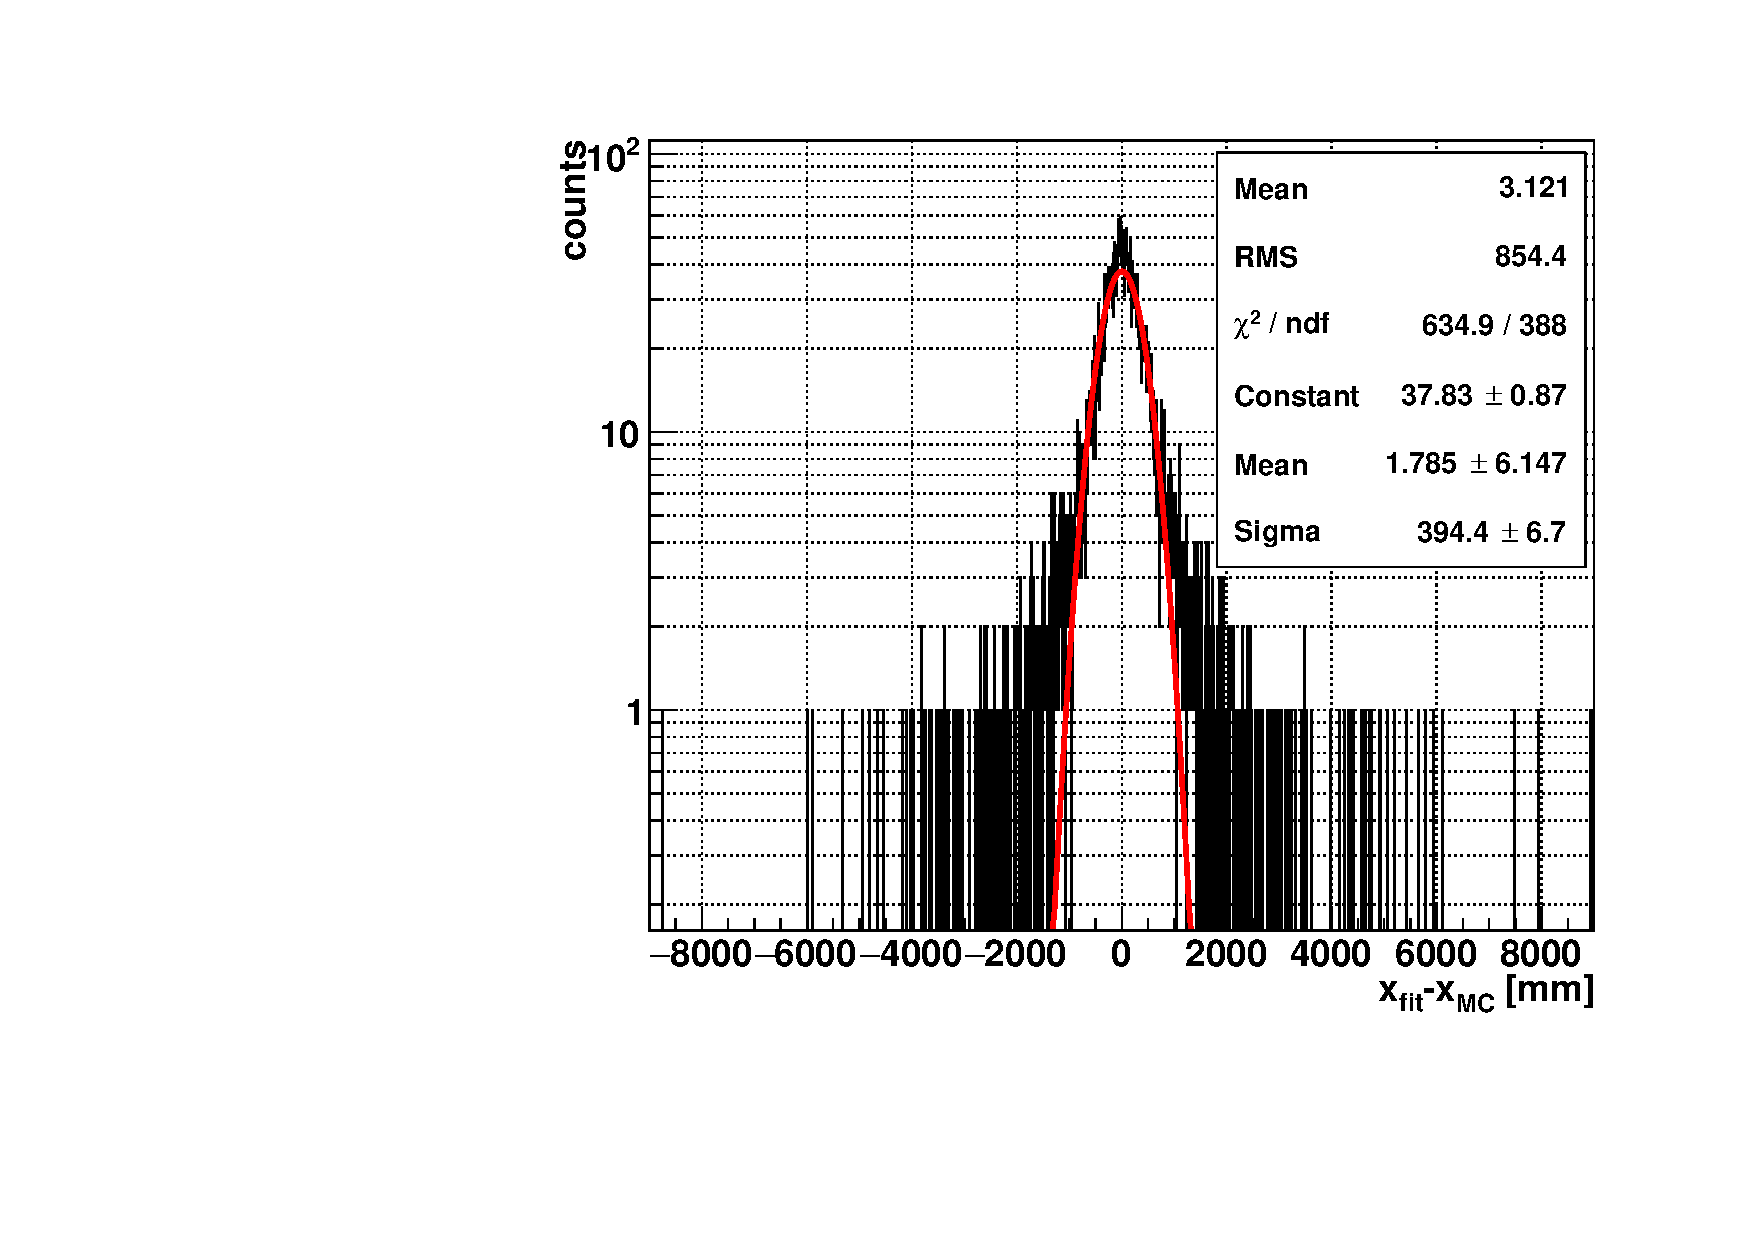
\includegraphics[width=6.5cm]{partial_bot_3MeV_xbias.pdf}
		\end{minipage}
	}   
	\subfigure[$y_{fit}-y_{mc}$.]{ 
		\begin{minipage}[t]{0.38\textwidth}
			\centering
			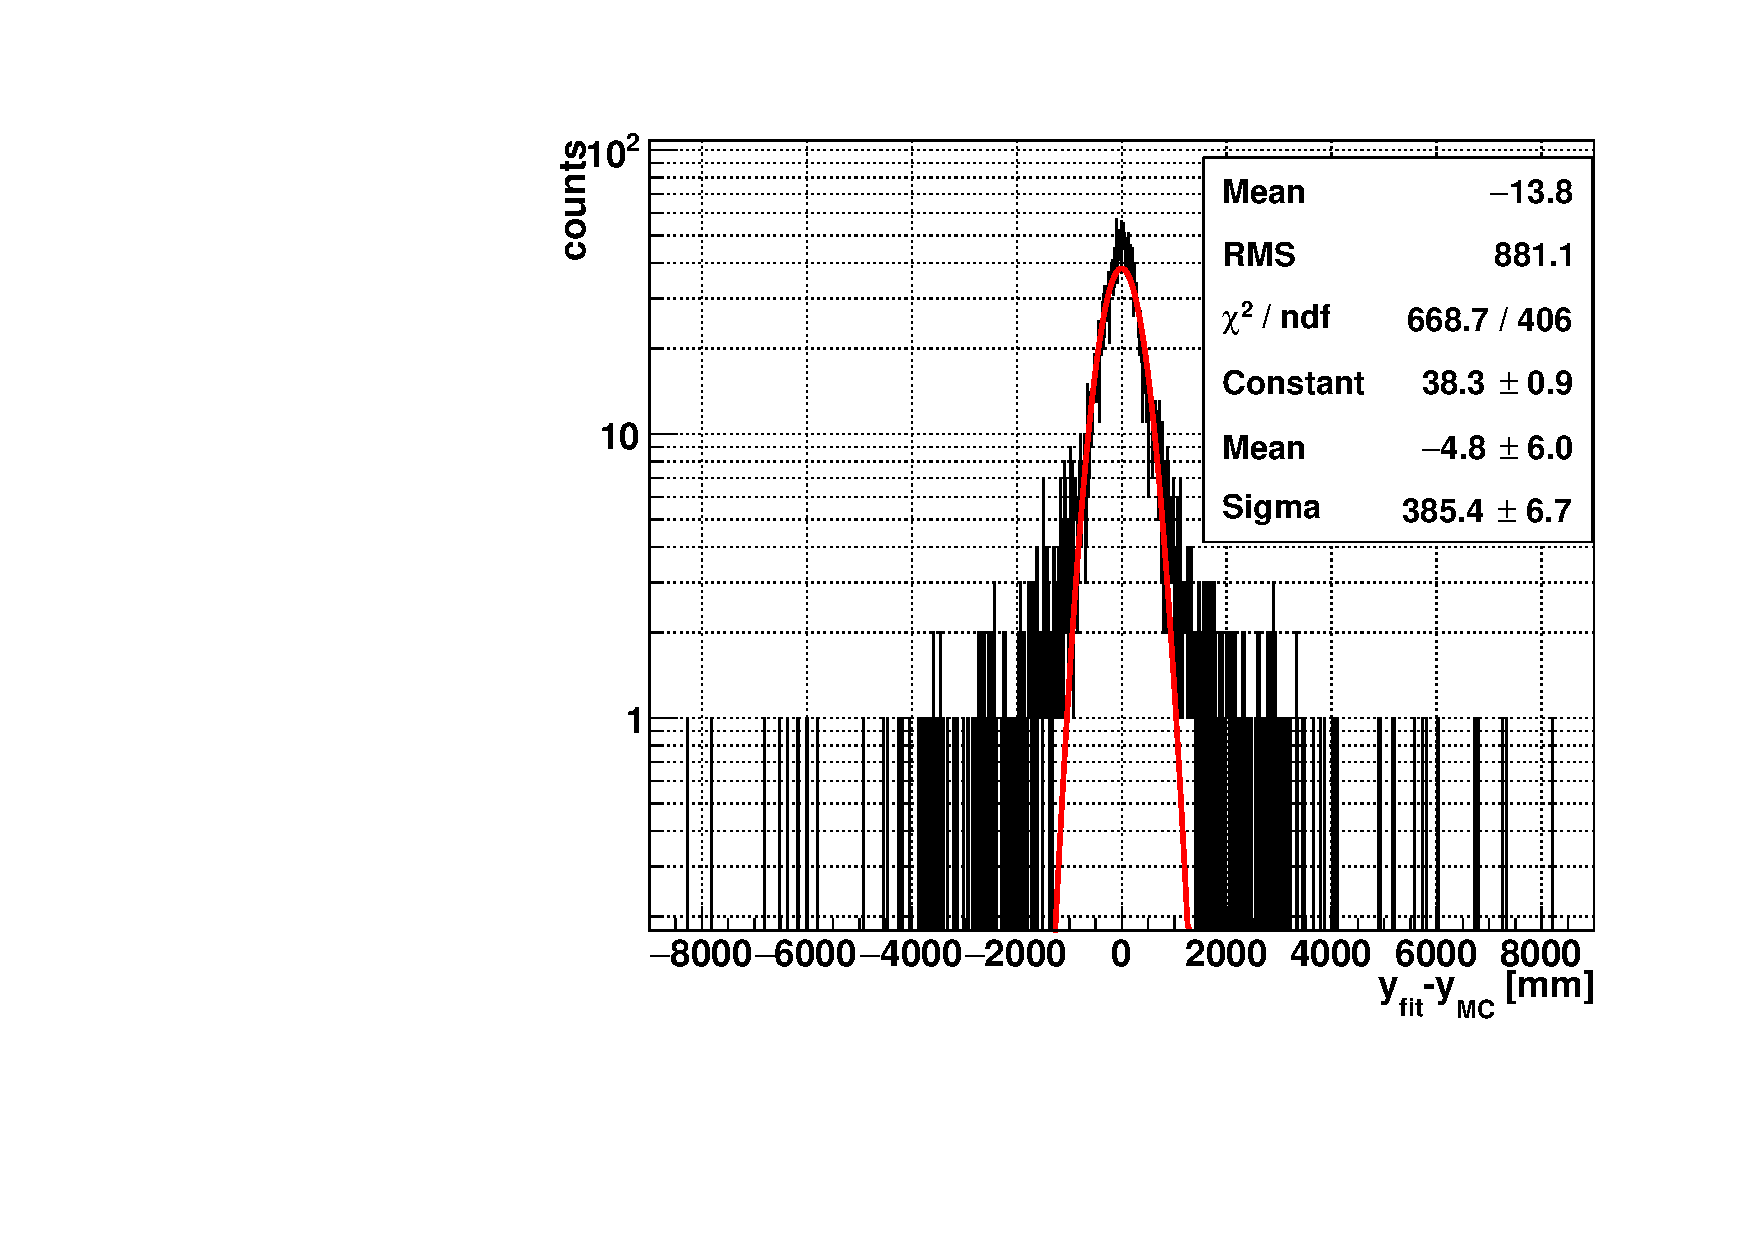
\includegraphics[width=6.5cm]{partial_bot_3MeV_ybias.pdf}
		\end{minipage}
	}
	\subfigure[$z_{fit}-z_{mc}$.]{ 
		\begin{minipage}[b]{0.38\textwidth}
			\centering
			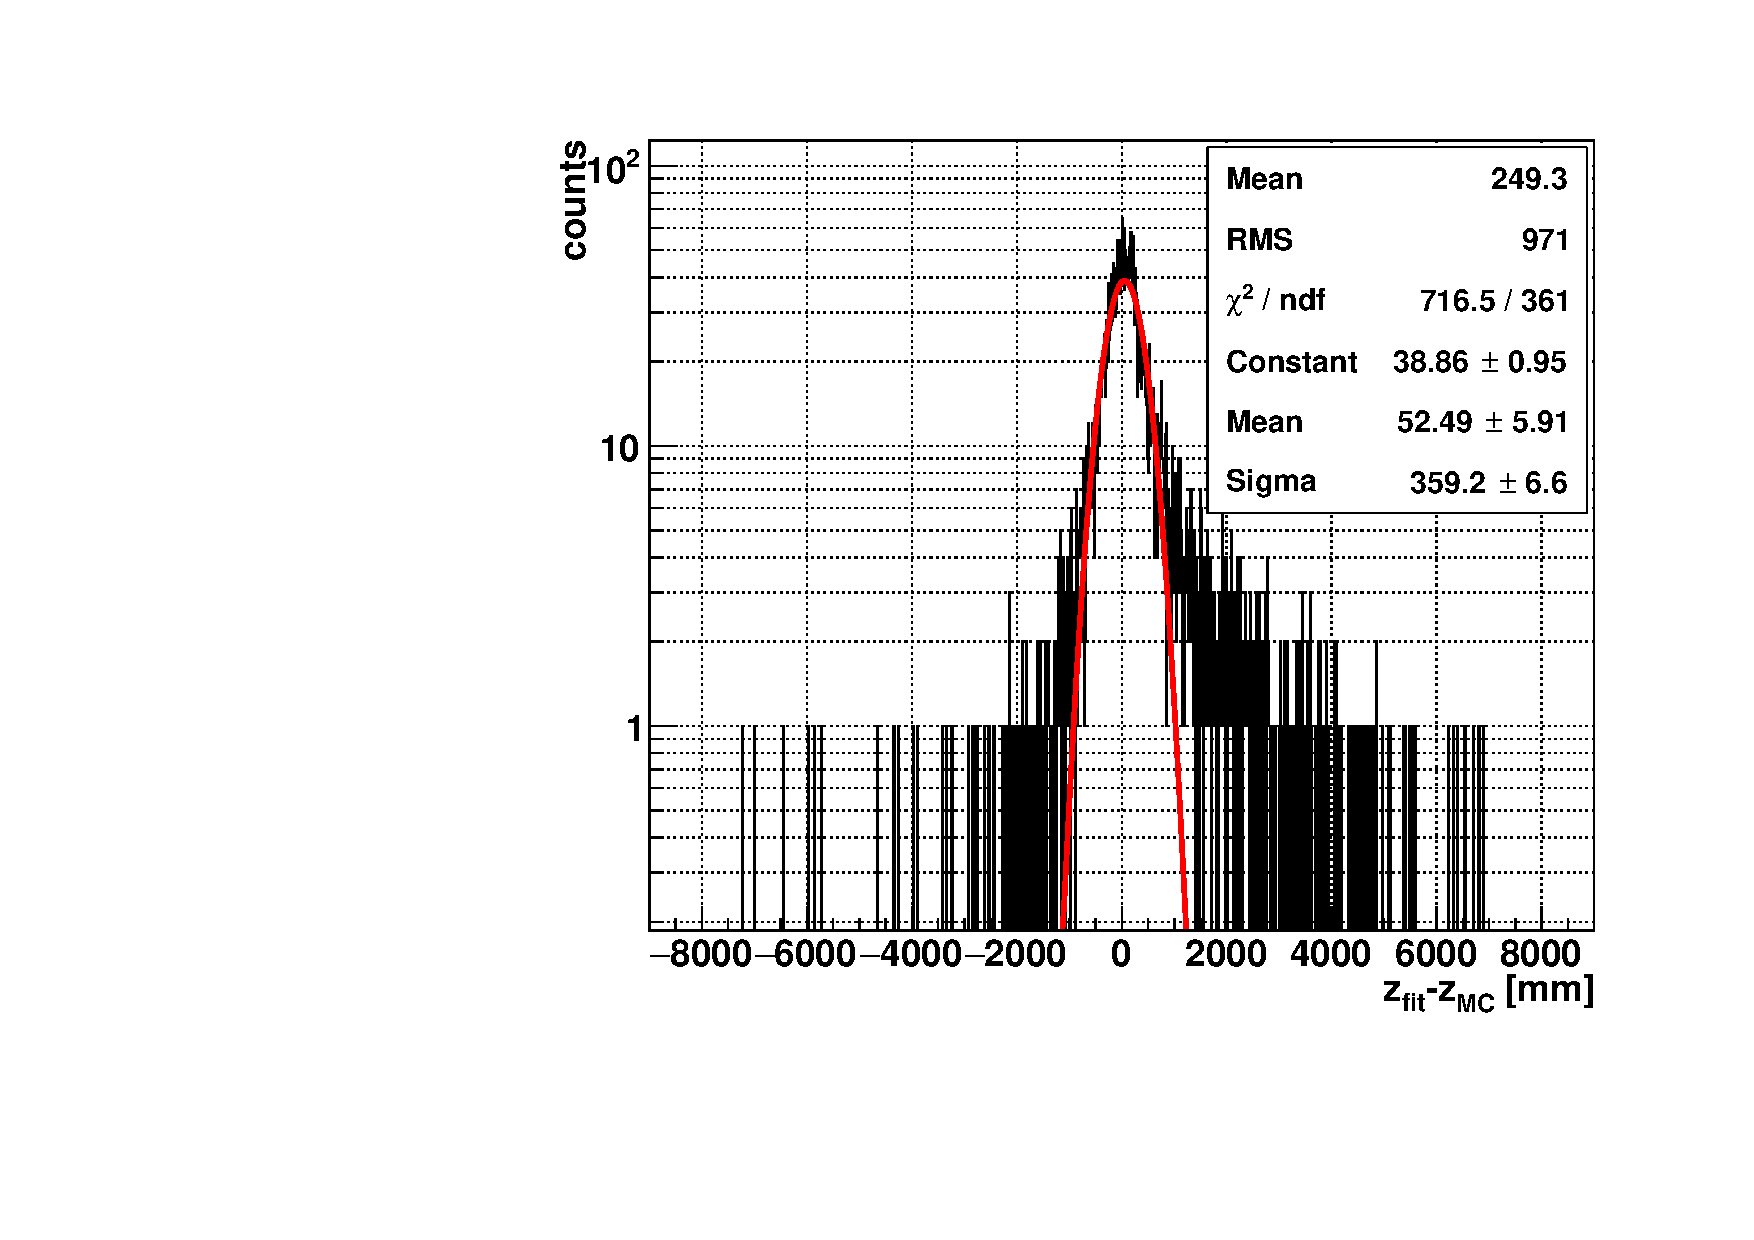
\includegraphics[width=6.5cm]{partial_bot_3MeV_zbias.pdf}
		\end{minipage}
	}
	\caption{Reconstructed positions and fit biases of the 3-MeV $e^-$ events in the water region.\label{fig:partial_inWater}}
\end{figure}

\subsubsection{Test on Different PPO Concentrations}\label{sect:ppoConcentration}

To study the effects of different PPO concentrations, in the partial-fill geometry, the water level was set at 3 m from the AV bottom, and the PPO concentrations were set to 0.25, 0.5, 1, 2, and 6 g/L respectively. Simulations of 5000 3-MeV $e^-$ were generated in the scintillator region with uniformly distributed positions and isotropic directions. The \texttt{MP scint-water fitter} uses the effective velocities and PDFs re-coordinated to the simulation geometries with corresponding PPO concentrations. The distributions of the position biases between the reconstruction and MC in x, y, and z axes were fitted with Gaussians to obtain the fit position biases ($\mu_{x,y,z}$) and resolutions ($\sigma_{x,y,z}$).

Fig.~\ref{fig:partialBiasVsPPO} and Fig.~\ref{fig:partialResolVsPPO} show the $\mu_{x,y,z}$ and $\sigma_{x,y,z}$ against PPO concentrations. Biases $\mu_{x,y,z}$ are stable in the [-15,15] mm region, while the resolutions ($\sigma_{x,y,z}$) improve (i.e. decrease) from about 150 mm to about 60 mm as the PPO concentration increases. The cause of this improvement in resolution is the higher light yield of the liquid scintillator with increasing PPO concentration, resulting in events causing larger NHits values and thus more information for the fitter. However the improvement from the 2 g/L case to the 6 g/L case is small, indicating a saturation effect for the PPO concentration above 2 g/L.

\begin{figure}[!htb]
	\centering
	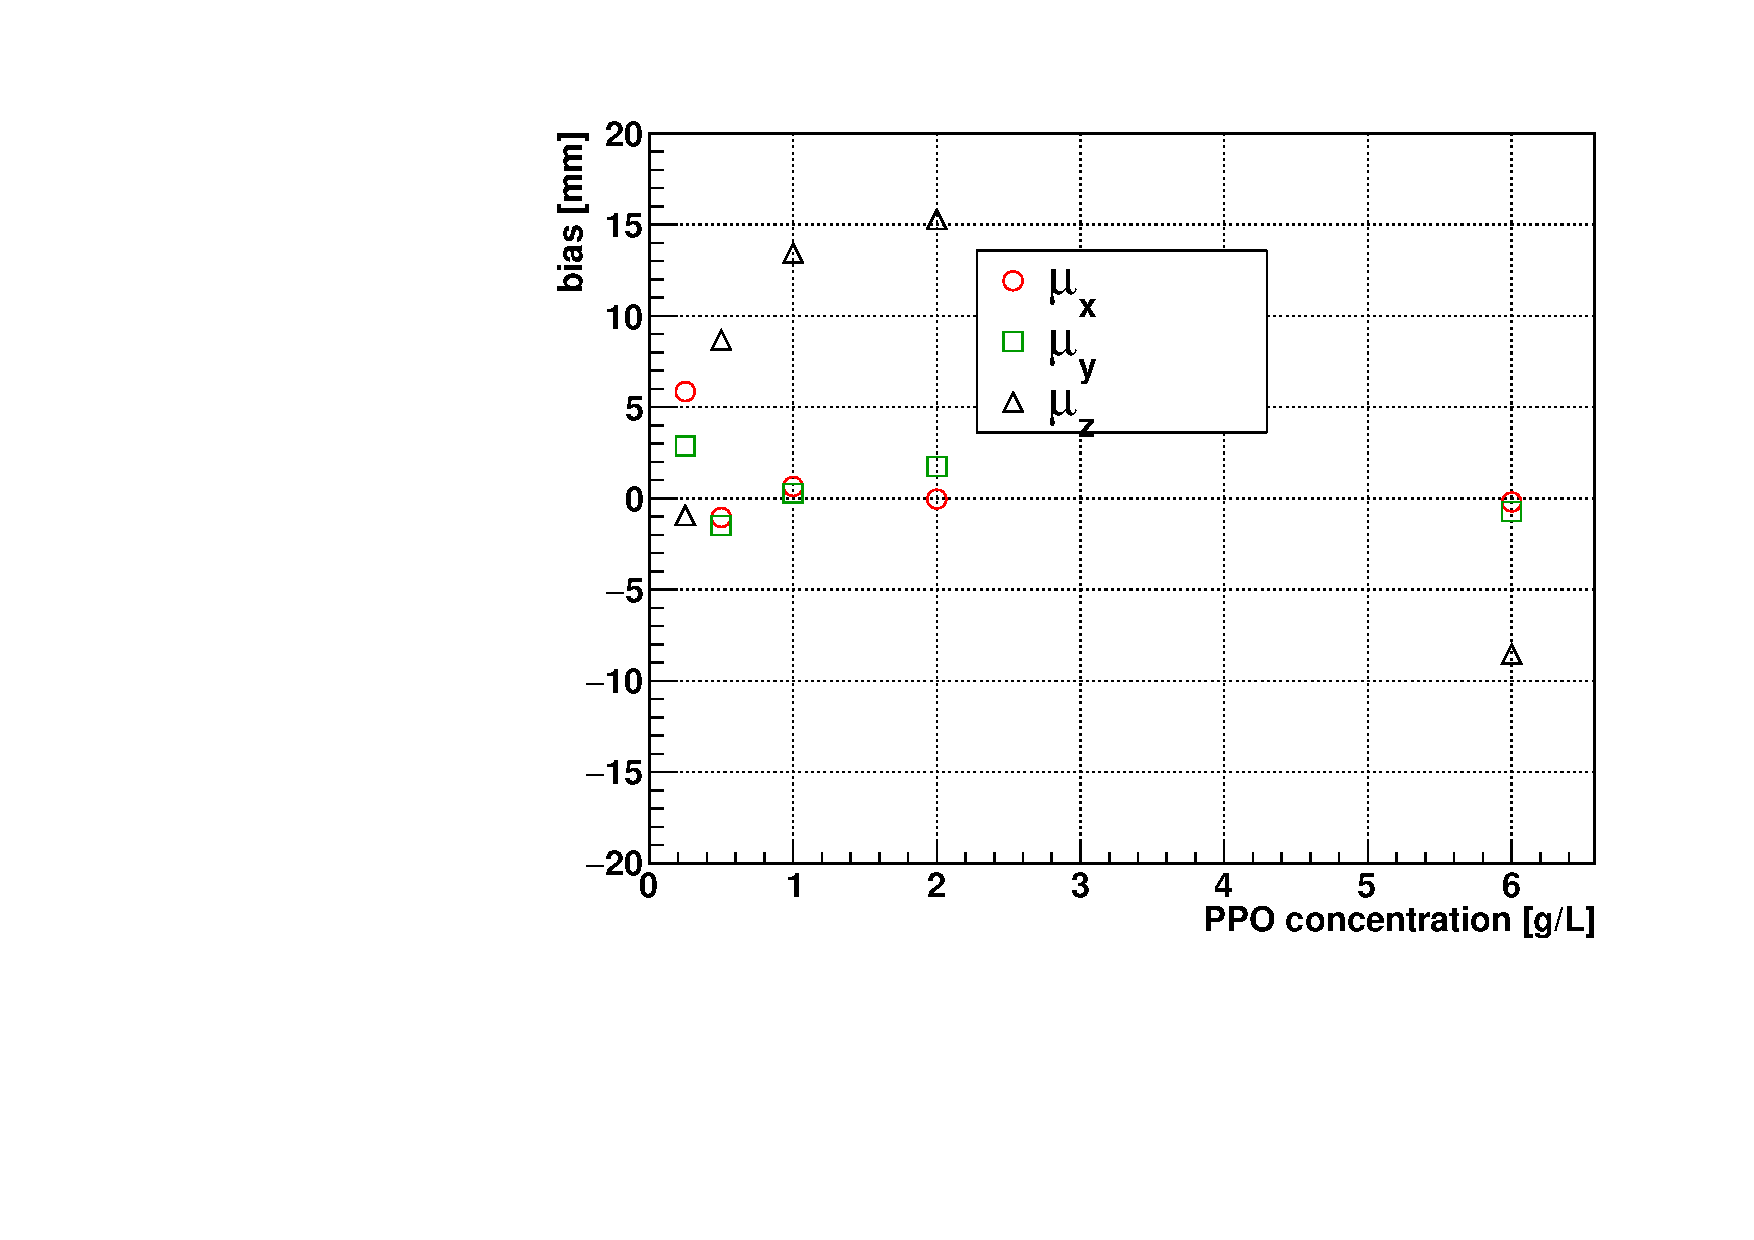
\includegraphics[width=10cm]{partialBiasVsPPO.pdf}
	\caption{Fit position biases against the PPO concentrations.	\label{fig:partialBiasVsPPO}}
\end{figure}

\begin{figure}[!htb]
	\centering
	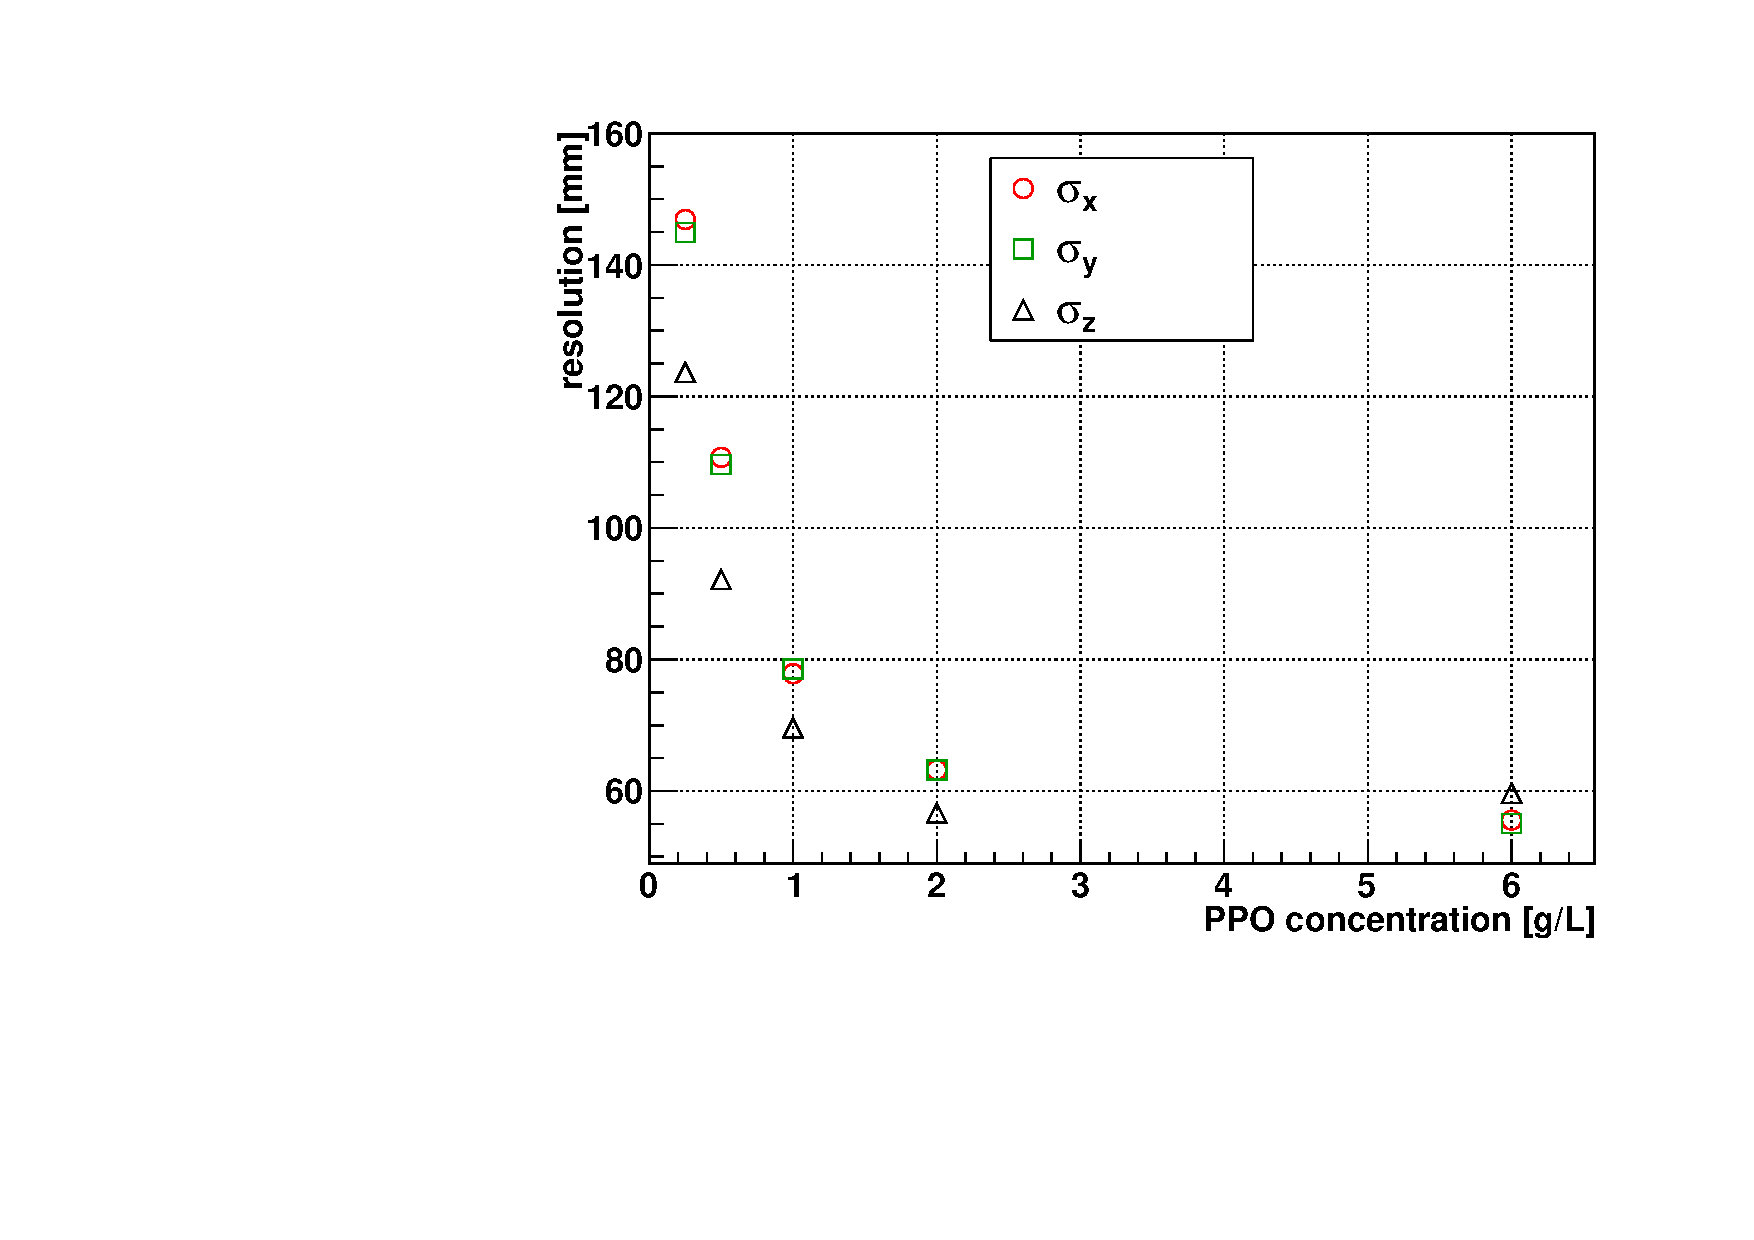
\includegraphics[width=10cm]{partialResolVsPPO.pdf}
	\caption{Fit position resolutions against the PPO concentrations.	\label{fig:partialResolVsPPO}}
\end{figure}

If using a timing PDF with the wrong PPO concentration for the reconstruction, the effect on reconstruction is small \cite{partialFitterPDFtestInvulnerable}. I simulated 3-MeV $e^-$ uniformly distributed in the LAB+0.25 g/L PPO scintillator with isotropic directions, and then reconstructed the events by using the timing PDFs for 0.5, 1 and 2 g/L PPO (higher concentrations) respectively. All of these reconstructions gave fitted positions close to the correct reconstruction using the 0.25 g/L timing PDF, with fit biases of about 5 mm on the three axes. On the other hand, by repeating the simulations but with LAB+2 g/L PPO and then reconstructing using the timing PDFs of 0.25, 0.5 and 1 g/L PPO (lower concentrations) respectively, I found the fit biases were still around 5 mm. This indicates that the fit provided by the \texttt{MP scint-water fitter} is indifferent to changes in PPO concentration. The implication is that if the true PPO concentration in the detector were slightly different from the nominal value assumed for reconstruction, the effect on the reconstruction would not be very significant.

\subsection{Test on Bi-Po Simulations}\label{sect:bipo}

Thorium-232 ($^{232}$Th) and Uranium-238 ($^{238}$U) are the two major internal contaminating isotopes (backgrounds) in the liquid scintillator. The amounts of these two backgrounds can be evaluated by a technique called ``Bi-Po analysis'', which hinges on tagging the $^{212}$Bi-$^{212}$Po event pairs from the $^{232}$Th decay chain and the $^{214}$Bi-$^{214}$Po event pairs from the $^{238}$U decay chain. This analysis is one of the crucial physics studies during the partial-fill phase. Here I tested the \texttt{MP scint-water fitter} on simulations of $^{214}$Bi-$^{214}$Po events in the detector with the LAB+0.5 g/L PPO and the interface at 4.5 m. In the $^{238}$U decay chain, $^{214}$Bi undergoes a $\beta^-$ decay, which can trigger a prompt event \cite{nndc}; its daughter $^{214}$Po, with a half-life of 164.3 $\mu$s, goes through $\alpha$ decay, and this can trigger a delayed event. Applying proper cuts on the position and time differences between the prompt and delayed events can effectively tag (identify) these $\beta-\alpha$ event pairs due to the $^{214}$Bi-$^{214}$Po decay sequence, allowing to evaluate the $^{238}$U level. An optimized algorithm was developed by the collaboration \cite{joshW1}, and a flowchart for picking the event pairs is shown in Fig.~\ref{biPo_flowchart} in Appendix.~\ref{appendix:bipo}.

%%  with a chance of 99.9791\% and the end-point energy at 3.27 MeV,  and the emitted 7.33-MeV $\alpha$ particle
This tagging algorithm was applied to reconstructed event vertices. Fig.~\ref{fig:214Bipo} shows the distributions of NHits for the tagged $^{214}$Po and $^{214}$Bi events. A clear and relatively narrow single peak shows the $\alpha$ events from the $^{214}$Po alpha-decay, and a wider and continuous spectrum shows the $e^-$ events from the $^{214}$Bi decay. Fig.~\ref{fig:parital_bipo214} shows the biases between the MC and the reconstructed positions, projected onto the $z$-axis. Fit errors on the three axes were fitted with Gaussians to obtain the biases and resolutions, which are listed in Table.~\ref{tab:partial_bipo214}. These results indicate that the fitter's performance is acceptable for the Bi-Po analysis in the partial-fill.

\begin{figure}[!htb]
	\centering
	\includegraphics[width=10cm]{214Bipo_4500mm0p5PPO.png}
	\caption[Distributions of NHits for the tagged $^{214}$Po and $^{214}$Bi events.]{Distributions of NHits for the tagged $^{214}$Po (dashed red line) and $^{214}$Bi (solid black line) events.	\label{fig:214Bipo}}
\end{figure}

\begin{figure}[htbp]
	\centering
	\subfigure[$z_{fit}-z_{MC}$ for tagged $^{214}$Bi.]
	{ 
		\begin{minipage}[b]{0.38\textwidth}
			\centering
			\includegraphics[width=6.5cm]{214Bi_Bipo214_deltaZ.pdf}
		\end{minipage}
	}
	\subfigure[$z_{fit}-z_{MC}$ for tagged $^{214}$Po.]{ 
		\begin{minipage}[b]{0.38\textwidth}
			\centering
			\includegraphics[width=6.5cm]{214Po_Bipo214_deltaZ.pdf}
		\end{minipage}
	}
	\caption[Fit position biases for tagged $^{214}$Bi and $^{214}$Po]{Fit position biases for tagged $^{214}$Bi (left) and $^{214}$Po (right).\label{fig:parital_bipo214}}
\end{figure}

\begin{table}[ht]
	\centering
	\caption{\label{tab:partial_bipo214} Fit position biases and resolutions for the $^{214}$Bi-$^{214}$Po tagging. Unit: mm.}	
	{\centering
		\begin{tabular*}{140mm}{c@{\extracolsep{\fill}}cccc}
			\toprule 
			Tagged isotope & $\mu_x\pm \sigma_x$ & $\mu_y\pm \sigma_y$ & $\mu_z\pm \sigma_z$\\
			\midrule
			$^{214}$Bi &  -7.657$\pm$127.2 & -2.071$\pm$129.6 & 2.041$\pm$114.5 \\
			$^{214}$Po &  -0.695$\pm$128.5 & -0.1355$\pm$129.3 & -22.21$\pm$103.0\\
			\bottomrule	
		\end{tabular*}
	}
\end{table}

\subsection{Discussions for the Partial Fitter}\label{sect:partialFitterDiscuss}

It was suggested by the SNO+ collaboration that I attempt to use the \texttt{MP scint-water fitter} to determine the water/scintillator interface level \cite{mpFitWaterLevel}. For this purpose the water level ($Z_\mathrm{water}$) is considered as an additional fit parameter so that the \texttt{MP fitter} fits for {\em five} parameters: $(x,y,z,t,Z_\mathrm{water})$. The bias between the true $Z_\mathrm{water}$ and the reconstructed value was fitted with a Gaussian, from which a bias of 40 mm and a resolution of 492 mm were deduced. The fit resolution for $Z_{\mathrm{water}}$ is much larger than the event position resolution, so this method is not good enough to be applied on the analysis.

The reconstructed vertices of certain events, such as the $^{214}$Bi-$^{214}$Po event pairs, can be used to calculate the time residual distribution, which is taken as the time profile caused by the $e^-$ or $\alpha$ particles in the liquid scintillator. By extracting the characteristic time constants from the time profile, the quality and optical properties of the liquid scintillator can be obtained. This analysis has been applied by the collaboration on the partial-fill data \cite{partialFillTres,partialFillBiPo214}.

To process the partial-fill data, the water level set in the \texttt{MP scint-water fitter} is intentionally moved down by 150 mm (a few centimeters larger than the resolution at 3 MeV) from the nominal water level. This was done to include some events mis-reconstructed in the water region, and then to include more events for a conservative background estimation for the liquid scintillator. 

To improve the performance of the \texttt{MP scint-water fitter}, two points have been suggested by the collaboration. They have not been applied or tested in this thesis, but they are worth future investigation:
\begin{itemize}
	\item The timing PDFs used by the \texttt{MP scint-water fitter} were obtained from bench-top measurements and the derivatives of the PDFs are alculated numerically. However, the PDFs can be expanded and fitted with suitable (e.g. Chebyshev) polynomials to obtain an analytic approximation function to describe the PDF\cite{press2007numerical}. Then the analytical function can give proper and smooth analytical derivatives, which may reduce the time cost of calculating the likelihoods using the numerical methods.	
	
	\item To refine the reconstruction algorithms by accounting for refracted and reflected light paths. Currently, possible event-PMT paths that entail refraction and/or reflection {\em are neglected}, to simplify the calculations, and the \texttt{MP scint-water fitter} (also the \texttt{MP scint fitter} to be discussed in the next section) simply uses the straight-line light paths from the event position to the hit PMTs. However, it obviously would be more realistic to account for the refracted and reflected light paths, since such paths necessarily exist due to the interface between the two different optical media, the water and the liquid scintillator. The Fresnel equations can be used for calculating the possibilities of these light paths\cite{partialWater}, although such calculations are complicated. Also, the influence on photon paths of the 5-cm thick AV, which is another optical medium, is totally neglected by the fitter. To take this into account, three different boundaries of optical media would have to be considered in calculations for refracted and/or reflected light paths, which is a complicated proposition. In this case, a trade-off between the accuracy \& precision of the reconstruction versus CPU time consumption comes into play.
\end{itemize}

\section{Vertex Reconstruction for the Scintillator Phase}\label{sect:scintFitter}

As mentioned in the previous section, the procedure for vertex reconstruction for the scintillator phase is similar to that for the partial-fill case, while no water-scintillator interface is considered here since the AV is fully filled with liquid scintillator. Only the ray-sphere and ray-cylinder intersections are calculated and thus the major code of the \texttt{MP scint fitter} was modified directly from the \texttt{MP scint-water fitter} by removing the ray-plane intersection calculations.

\subsection{Performance of the Vertex Reconstruction}

Since a 2.5 MeV event is the signal of major interest in the scintillator and tellurium-loading phases, a few tests were focused on this energy. Simulations of 10,000 2.5 MeV $e^-$ events were generated at random positions inside the AV, and with isotropic directions. Fig.~\ref{fig:scintIsoFill_2p5MeV} shows the distributions of the position biases between the reconstruction and the MC truth. These distributions were fitted with Gaussians to obtain the mean error or bias ($\mu$) and resolution ($\sigma$). It can be seen that the fit position biases lie within the region of $[-2,2]$ mm, while the resolutions are better than 70 mm on all axes: $\mu_{x,y,z}\in(-2,2)$ mm and $\sigma_{x,y,z}<70$ mm.

\begin{figure}[htbp]
	\centering
	\subfigure[$x_{fit}-x_{mc}$]{
		\begin{minipage}[t]{0.38\textwidth}
			\includegraphics[width=6cm]{fullScint_2p5_xbias.png}
		\end{minipage}
	}   
	\subfigure[$y_{fit}-y_{mc}$]{ 
		\begin{minipage}[t]{0.38\textwidth}
			\centering
			\includegraphics[width=6cm]{fullScint_2p5_ybias.png}
		\end{minipage}
	}
	\subfigure[$z_{fit}-z_{mc}$]{ 
		\begin{minipage}[b]{0.38\textwidth}
			\centering
			\includegraphics[width=6cm]{fullScint_2p5_zbias.png}
		\end{minipage}
	}
	%\includegraphics[width=6cm]{fullscint_2p5MeV_radialBias.png}
	\caption[The fit position biases projected on the x, y and z axes, for 2.5-MeV $e^-$ in full scintillator simulations.]{The fit position biases projected on the x, y and z axes, for 2.5-MeV $e^-$ in full scintillator simulations. The distributions were fitted with Gaussian functions.\label{fig:scintIsoFill_2p5MeV}}
\end{figure}

A test of the quality of vertex reconstruction versus event radial position was performed, and this was similar to the tests in the Sect.~\ref{sect:waterFitterVertex}. In simulations, 2.5 MeV $e^-$ were generated within each of eleven thin concentric shells. Fig.~\ref{fig:scintShellVsBias} and Fig.~\ref{fig:scintShellVsResol} respectively show the biases ($\mu$) and resolutions ($\sigma$) as a function of radius: for all values of event radial position ($R$), $\mu_{x,y,z}\in(-10,5)$ mm and $\sigma_{x,y,z} < 70$ mm. 

\begin{figure}[!htb]
	\centering
	\includegraphics[width=10cm]{shellTestScintFitter_RvsBias.pdf}
	\caption[The Gaussian biases ($\mu$) of the \texttt{MP scint fitter} fit position biases as a function of radius, for the x, y, and z axes.]{The Gaussian biases ($\mu$) of the fit position biases as a function of radius, for the $x$- (red circle), $y$- (green square), and $z$- (black triangle) axes.}
	\label{fig:scintShellVsBias}
\end{figure}

\begin{figure}[!htb]
	\centering
	\includegraphics[width=10cm]{shellTestScintFitter_RvsResol.pdf}
	\caption[The Gaussian resolutions ($\sigma$) of the \texttt{MP scint fitter} fit position biases as a function of radius, for the $x,y,z$  axes.]{The Gaussian resolutions ($\sigma$) of the fit position biases as a function of radius, for the $x$- (red circle), $y$- (green square), and $z$- (black triangle) axes.}
	\label{fig:scintShellVsResol}
\end{figure}

For other energies (from 1 to 10 MeV), the Gaussian means and resolutions of the fit position biases are shown in Fig.~\ref{fig:scintBiasVsE} and Fig.~\ref{fig:scintResolVsE}. For the 1 MeV $e^-$ event, the $\sigma_{x,y,z}$ are below 85 mm. These resolutions are slightly better than the Borexino spatial resolution of $\sigma_{x,y,z} \sim 110$ mm for a 1 MeV electron at the detector center\cite{borexino2020experimental}.

\begin{figure}[!htb]
	\centering
	\includegraphics[width=10cm]{fullScintBiasVsE.pdf}
	\caption[The Gaussian means ($\mu$) of the \texttt{MP scint fitter} fit position biases as a function of energy, for the x, y, and z axes.]{The Gaussian means ($\mu$) of the fit position biases as a function of energy, for the x (red circle), y (green square), and z (black triangle) axes.}
	\label{fig:scintBiasVsE}
\end{figure}

\begin{figure}[!htb]
	\centering
	\includegraphics[width=10cm]{fullScintResolVsE.pdf}
	\caption[The Gaussian resolutions ($\sigma$) of the \texttt{MP scint fitter} fit position biases as a function of energy, for the x, y, and z axes.]{The Gaussian resolutions ($\sigma$) of the fit position biases as a function of energy, for the x (red circle), y (green square), and z (black triangle) axes.}
	\label{fig:scintResolVsE}
\end{figure}

\section{Multi-path Fitter Structure for Multiple SNO+ Physics Phases}

The \texttt{MP fitter} has already been implemented into the \texttt{RAT} software for data processing and analysis. Following the \texttt{RAT} event reconstruction structure, the \texttt{MP fitter} is suitable for multiple SNO+ physics phases. 

The \texttt{MP fitter} first loads the fitter database, which contains the parameters used by the fitter. Parameters includes the physical constants (e.g., speed of light); geometrical parameters of the detector (e.g., $r_\mathrm{PSUP}$, length of neck, water level); fitter setting parameters (e.g., the effective group velocity, fitter iteration number, etc.); and various optimized PDFs. This collection of parameters (and others not mentioned) is known as the \texttt{RAT} database (ratdb), stored in a \texttt{JSON} format\cite{JSONwiki}, and contains tables which are structured by different indices to indicate specific physics phases or detection media. For example, for the partial-fill phase with a PPO concentration of 0.5 g/L, the fitter extracts the PDFs and fitter setting parameters under the index of ``\texttt{labppo\_0p5\_scintillator}''. These fitter setting parameters and PDFs were optimized for the 0.5 g/L PPO partial-fill geometry.

After loading the database the \texttt{MP fitter} goes through the event-by-event reconstruction. For a triggered event, it calls PMT selectors and sends the timing and charge information of the selected PMTs to a \texttt{Likelihood Calculation Class}. Sect.~\ref{sect:PMTselector} will give the details about the PMT selectors. In the \texttt{Likelihood Calculation Class}, there are four main likelihood calculation functions\footnote{The \texttt{AirWaterVertex} for the early partial water fill test in 2014 and the \texttt{WavelengthShifterVertex} for the conceptual wavelength-shifter test, as mentioned in the previous sections, were not included in the current version of \texttt{RAT} since they are not used in actual physics phases.}: the \texttt{WaterVertex} and \texttt{WaterDirection} for the event vertex and direction reconstruction in the water phase; the \texttt{ScintWaterVertex} for vertex reconstruction in the partial-fill phase; and the \texttt{ScintVertex} for vertex reconstruction in the scintillator and tellurium-loading phases.

Reading the detector geometry settings and the assigned index of detection medium, the fitter selects proper likelihood functions to construct the likelihood functions and to calculate the likelihoods and their derivatives by evaluating fit parameters based on different light path calculations in different detector geometries. The calculated likelihoods and derivatives are sent to the MRQ method class to maximize the likelihood and find the best-fit values. The MRQ method class does not ``care'' about how the likelihood functions had been constructed nor how the likelihoods and derivatives had been calculated. 
	
A \texttt{Dump Likelihood Class} stores the trial fit parameters with respect to their likelihoods and derivatives for interesting events, by registering their event GTIDs in the database. By looking at the likelihood surfaces and derivatives of the event of interest, the fit performance for that event can be checked to see whether the fitter finds the global or local maximum. Sect.~\ref{appendix:likelihoodSurface} shows an example of the dumped likelihood surfaces and derivatives for an $^{16}$N event vertex reconstruction. 

Once the reconstructed results are obtained, the fitter will send them to the classifiers for further analysis. 

\section{Energy Reconstruction}\label{sect:energyFitter}

The SNO+ energy reconstruction algorithms (energy fitters) were based on SNO\cite{boulay2004direct,moffat2001optical} and have been further developed and optimized\cite{jones2011background,walker2016study,energyRSP}. 

The energy fitters mainly use lookup tables to convert the NHits value of a triggered event into reconstructed energy. The energy fitters used in the water phase are mainly the energy response processor (\texttt{EnergyRSP fitter}) \cite{walker2016study,boulay2004direct,moffat2001optical} and the energy Lookup fitter (\texttt{EnergyLookup fitter}) \cite{jones2011background,energyFunctional}. The \texttt{EnergyRSP fitter} is used to reconstruct the events inside the AV (internal events). It considers detailed detector effects, such as the asymmetric geometry of the detector, the optical response of each PMT (including the PMT detection efficiency, transmission probability, attenuation, etc.), and utilizes the reconstructed event positions, directions, and time residuals as inputs to convert the corresponding value of NHits to estimated energy based on simulation models and calibration data. The \texttt{EnergyLookup fitter} is simpler and is mainly used to reconstruct events in the cavity water (external events). It mainly uses the lookup table of the NHits dependence on the event reconstructed position from simulations to calculate the energy of the event \cite{jones2011background}. For the scintillator phase, a method using a functional form based on simulations was developed by Ref.~\cite{energyFunctional,energyRThetaFunctional} and is currently used in the \texttt{EnergyRThetaFunctional fitter}. All these fitters adapt to the true number of online PMTs for a particular physics run (or called ``channel efficiency''). 

The resolutions and scales of the reconstructed energies in the water phase were derived from the $^{16}$N calibration scans at certain detector points, a topic that will be covered in Chapter 5.

\subsection{Energy Figure of Merit}\label{sect:energy_fom}

The SNO+ Antineutrino working group developed three figure of merit (FoM) quantities for the energy fitters in the water phase to identify poorly reconstructed results which have significant biases to the truth energy values, especially for the low energy region around 2.2 MeV, which helps the analysis of neutron capture\cite{waterFoM,waterunidoc}. The following energy FoMs were applied to the energy reconstruction results during the water phase, which will be discussed in the next chapter. Brief descriptions are presented below, while more details can be found in Ref.~\cite{waterunidoc}.

\begin{itemize}
	\item[$\bullet$]$U$-test ($U_{test}$):
	a Mann-Whitney score uses the channel hit probabilities calculated by \texttt{EneryRSP} which are ordered and ranked. \texttt{EneryRSP} calculates the $N$ as the prompt NHits, and $N_{active}$ as the total number of active channels. For each active channel, the smallest hit probability assigned rank 1 and largest $N_{active}$. $S$ is a sum of assigned ranks for hit PMTs and $S\equiv \sum_{i}^N \mathrm{rank}_i$.
	\begin{equation}
	U_{test}\equiv \frac{S-N(N+1)/2}{N(N_{active}-N)},
	\end{equation}

	\item[$\bullet$] $G$-test ($G_{test}$):
 	a score that uses the hit probabilities from \texttt{EnergyRSP} ($E_i$), which are normalized to the number of observed hits ($N$):
	\begin{equation}
	G_{test}\equiv \frac{1}{N}\sum_{i=1}^N \log(\frac{1}{E_i}),
	\end{equation}
	
	\item[$\bullet$] $Z$-factor ($Z_{factor}$):
	a score that uses the medians and median absolute deviations of hit probabilities from \texttt{EnergyRSP}:
	\begin{equation}
     Z'\equiv 1-\frac{3(\sigma_p+\sigma_n)}{\mu_p-\mu_n},
    \end{equation}
    where $\mu_p$ is the median probability of all active PMT channels with hits; $\mu_n$ is the median probability of all active PMT channels; $\sigma_p$ is the median absolute deviation of hit PMT probability distribution; and
    $\sigma_n$ is median absolute deviation of PMT probability distribution.
\end{itemize}

\subsection{Energy Reconstruction in Partial-fill Phase}

At the time this thesis was written, no suitable energy fitter had yet been provided for the partial-fill phase. Below I will describe two methods that I have investigated for energy reconstruction in the partial-fill phase: the NHits-scale method, based on Ref.~\cite{partialEnergy} and the NHits-ratio method, based on Ref.~\cite{partialEnergyYang}. Both methods use look up tables produced by simulations of $e^-$ events in the partial-fill geometry, then compare with the case in the full-fill geometry, and scale the energy. Both, however, will need further effort if they are to produce well-defined results \cite{jiePartialEnergy,jiePartialEnergyNhitRatio}.

In the NHits-scale method, for an $e^-$ event at (0,0,z) with a fixed energy (values of 1 MeV and 2.5 MeV were tested), a scaling factor ($S$) between its NHits value in the partial-fill (NHits$_\mathrm{partial}$) with a water level $Z_\mathrm{water}$ set in the simulation and the NHits value in the full-fill (NHits$_\mathrm{full}$) is defined as
\begin{equation}
S = \mathrm{\frac{NHits_{partial} - NHits_{full}}{NHits_{full}}} = 0.33 \, a_0 \, \left( Z_\mathrm{water} + 6005 \right)^{2.76} \; ,
\end{equation}
where the final term is an empirical function and the fit parameter $a_0$ depends on the different event $z$ positions in the simulations. Then the energy in the partial-fill is found by $E_\mathrm{partial} = E/(1 + S)$ \cite{partialEnergy, jiePartialEnergy}.
 
In the NHits-ratio method, the NHits value of an $e^-$ event at (0,0,0) mm in the full scintillator geometry was used as a reference (NHits$_\mathrm{ref}$). By simulating 1 to 10 MeV $e^-$ events (with a 1 MeV step) in the full-fill geometry with 0.5 g/L PPO, and fitting the NHits to the energies, a converting function between the energy and NHits was found \cite{jiePartialEnergyNhitRatio}: 
\begin{equation}
E_\mathrm{full} = f(\mathrm{NHits})=0.051+0.003\cdot \mathrm{NHits}+2.49\times 10^{-7}\cdot \mathrm{NHits} \; .    
\end{equation}
Then for the partial-fill geometry with a given $Z_\mathrm{water}$, $e^-$ events were simulated at different $(\rho=\sqrt{x^2+y^2},z)$ positions in the AV, with $\rho$ ranging from 0 to 5500 mm with a step of 500 mm, and $z$ ranging from -5500 to 5500 with a step of 500 mm (these ranges cover the AV volume of interest). The value of scaled NHits for an event at $(\rho_0,z_0)$ is found by
\begin{equation}
\mathrm{NHits' = NHits_{partial}/(NHits(\rho_0,z_0)/NHits_{ref})} \; ,
\end{equation}
and finally the partial energy is found as $E_\mathrm{partial} = f(\mathrm{NHits'})$ \cite{jiePartialEnergyNhitRatio}.

\section{Machine Learning and Deep Learning}

Nowadays, the vast amount of data available to particle experiments make it feasible to implement machine learning and deep learning methods for data analysis. Chapter 6 will describe a machine learning method applied to solar neutrino analysis. At the time of writing, a deep learning framework is being developed for reconstruction\cite{markMachineLearning,markNeuralTalk,markNeuralNetwork}. This method investigates the relation between the hit PMT distributions and the event reconstruction, currently for the position and direction. It trains neural networks based on information from MC simulation datasets (with $\mathcal{O}(10^6)$ events) and from calibration datasets, to yield an algorithm that predicts event position and direction\cite{markNeuralTalk}. A few physics-based loss functions (or called ``cost-functions''), such as the loss function checking the $t_\mathrm{res}$, can be added to improve the reconstruction performance\cite{markNeuralTalk}. 

Once the neural networks are trained, the reconstruction speed is expected to be from 100 to 1000 times faster than the traditional likelihood-fit method when running on the CPU (Central Processing Unit). In addition, since the deep learning method can utilize the computing power of the GPU (Graphics Processing Unit), it is expected to be $10^4$ times faster \cite{markNeuralTalk,markNeuralNetwork}. Such a rapid reconstruction is hoped to be applied in the scintillator phase, for which the existing likelihood-based fitters will be very time-consuming owing to the higher NHits events. The deep learning framework is expected also to aid the data analysis.

\section{Conclusion}

The Multi-path Fitter framework for event vertex reconstruction was developed for multiple SNO+ physics phases. Under this framework, the \texttt{MP water fitter} works as an alternative fitter to provide additional reconstruction information for water data, and it gives good position and direction resolution for the water analysis. The \texttt{MP scint-water fitter} works as the prime fitter for the SNO+ partial-fill phase.
